\chapter{Projekt}

\section{Przypadki użycia}
\todo{diagram przypadków użycia}

\begin{minipage}{\textwidth}
    \begin{figure}[H]
        \centering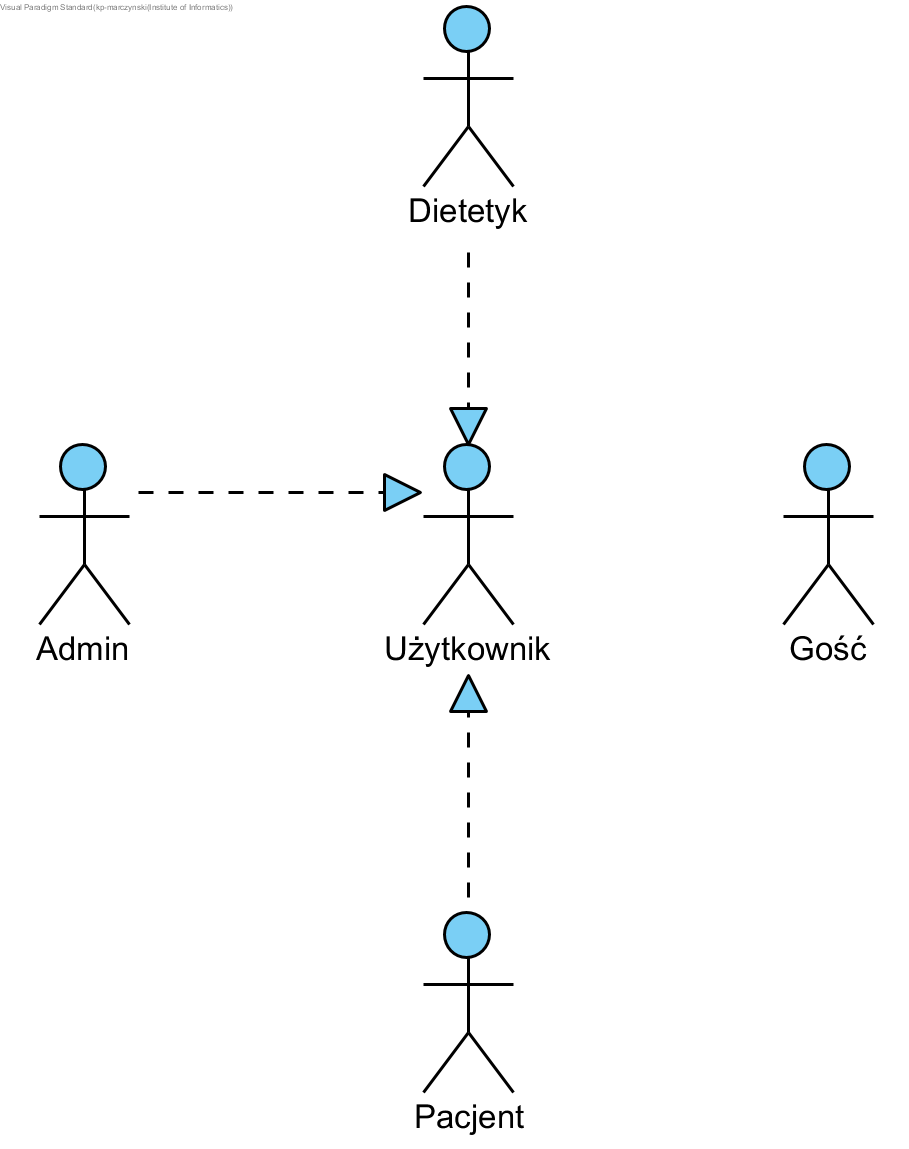
\includegraphics[scale=0.55]{../uml/use_case_diagrams/users.png}
        \caption{Użytkownicy - diagram przypadków użycia (opr.wł).}\label{rysunek:use-case-diagram-users}
    \end{figure}
\end{minipage}

\begin{minipage}{\textwidth}
    \begin{figure}[H]
        \centering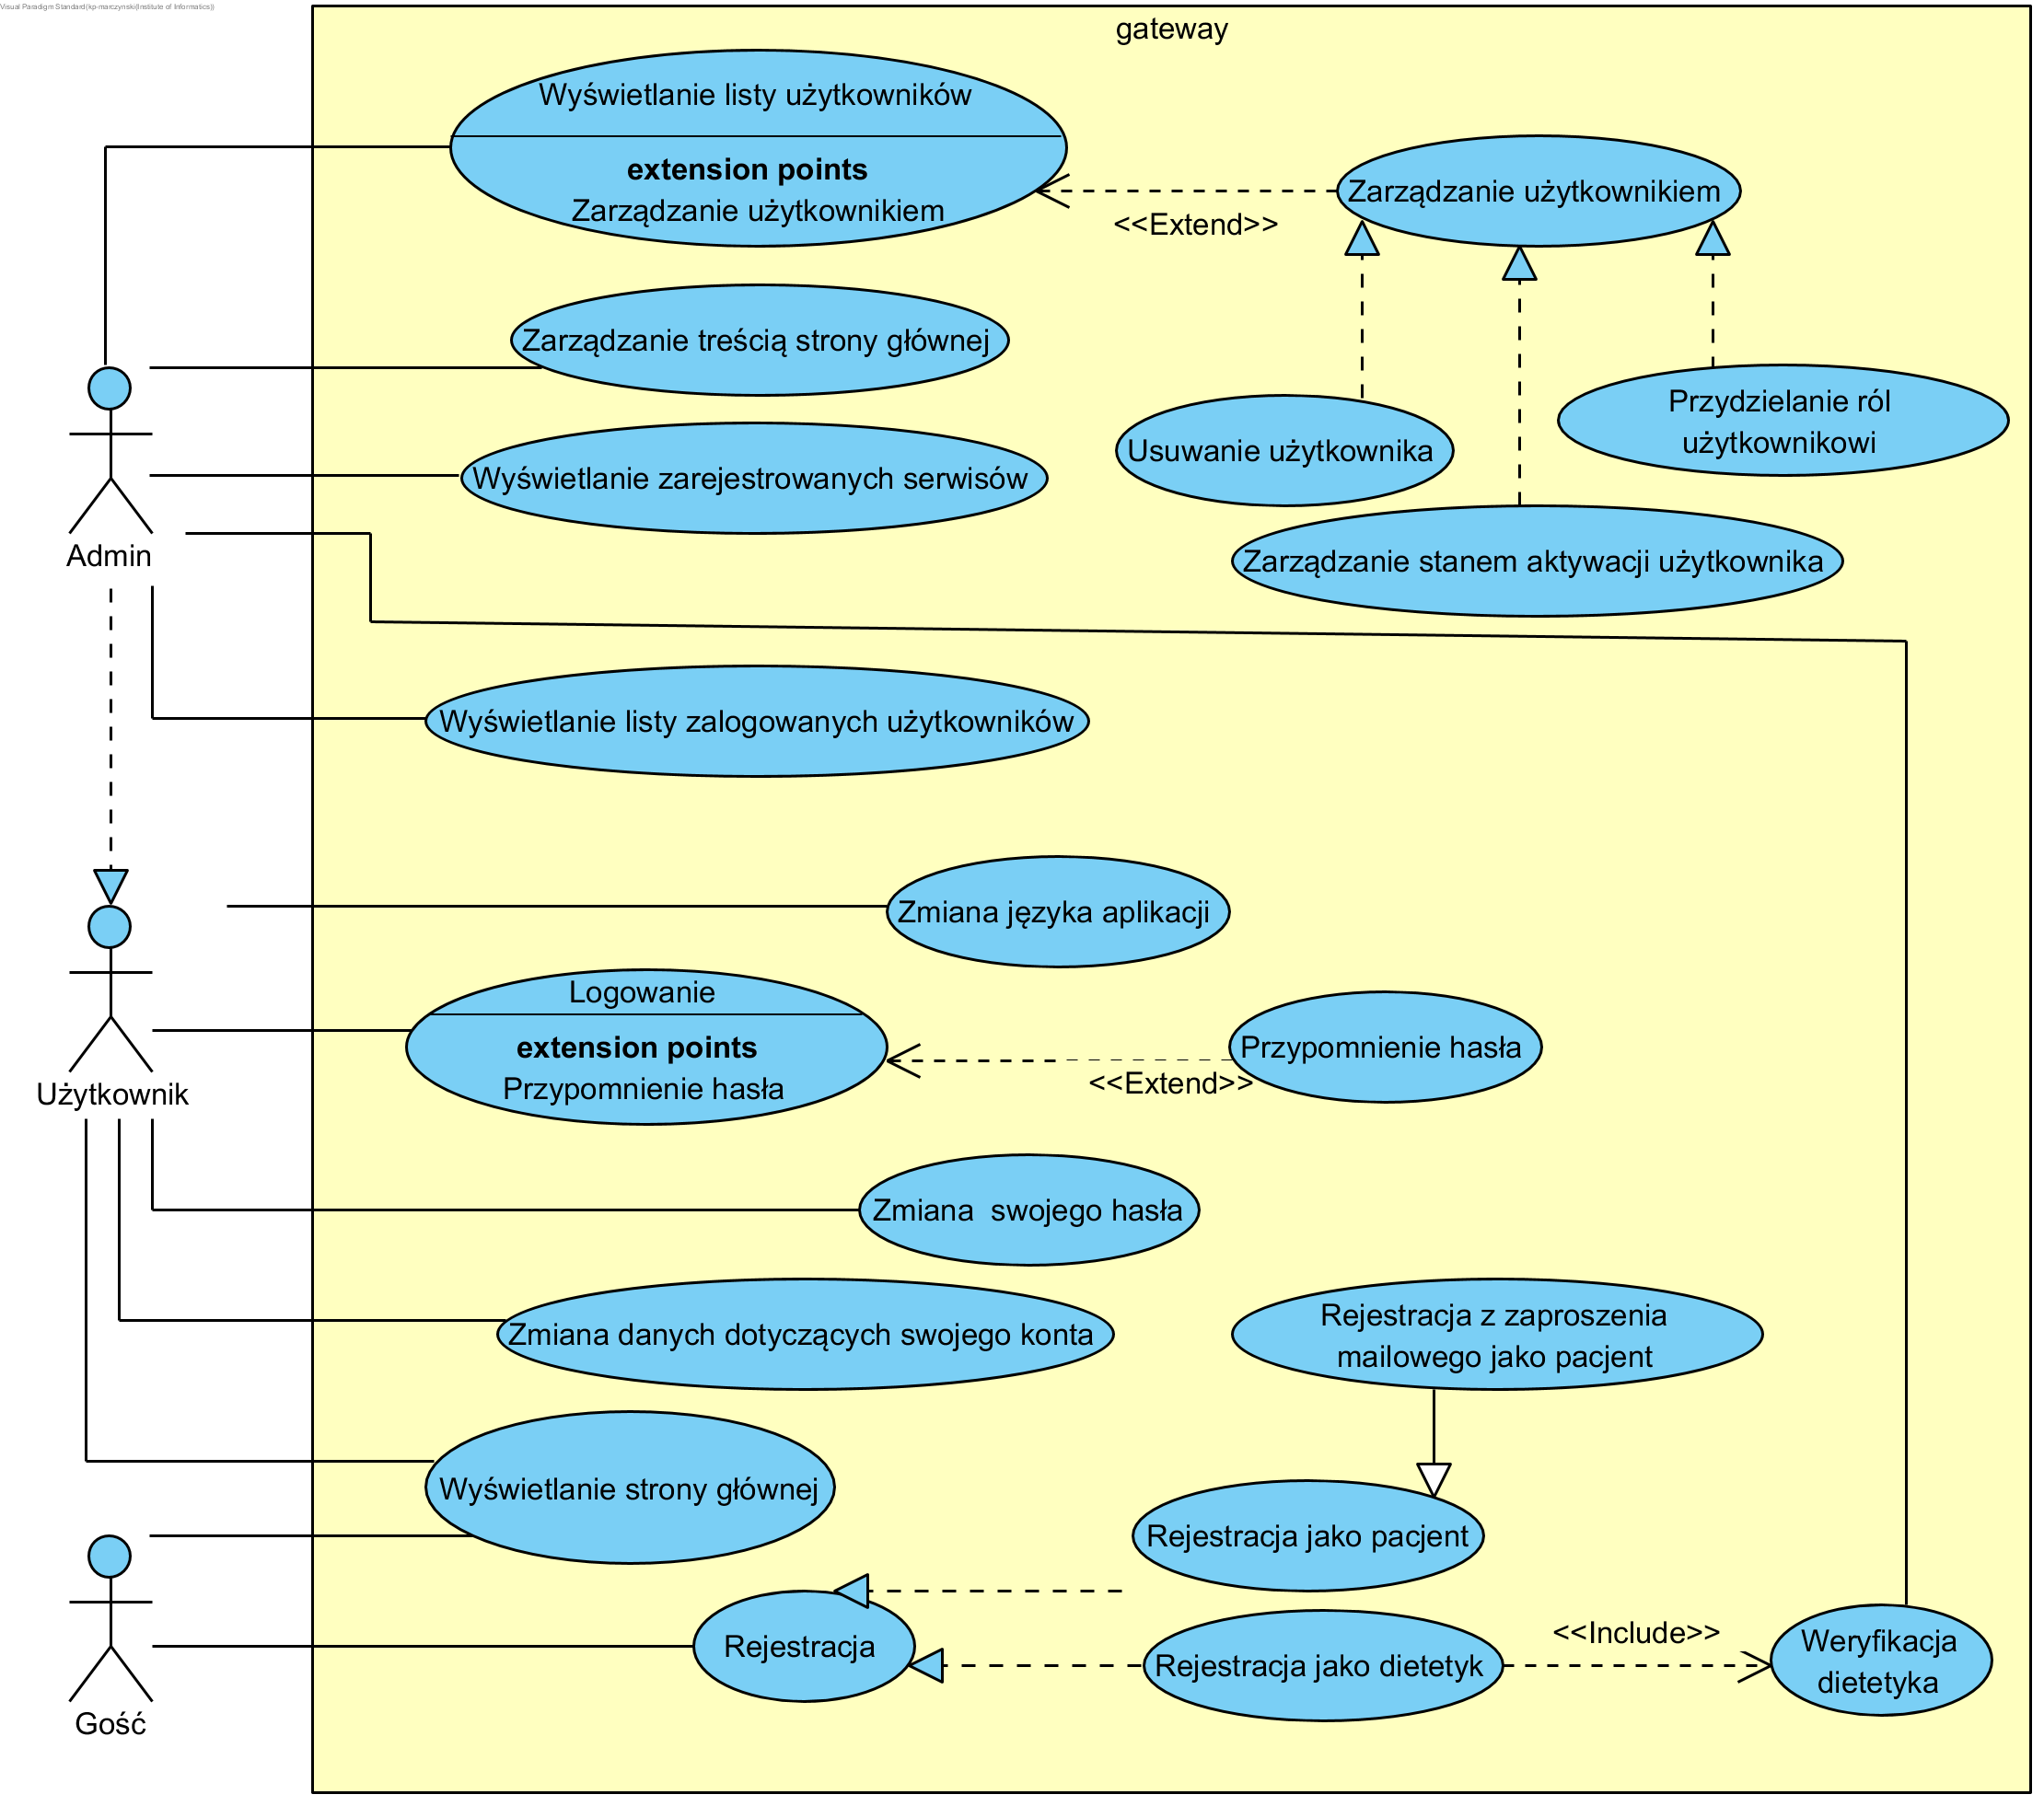
\includegraphics[scale=0.55]{../uml/use_case_diagrams/gateway.png}
        \caption{Gateway - diagram przypadków użycia (opr.wł).}\label{rysunek:use-case-diagram-gateway}
    \end{figure}
\end{minipage}

\begin{minipage}{\textwidth}
    \begin{figure}[H]
        \centering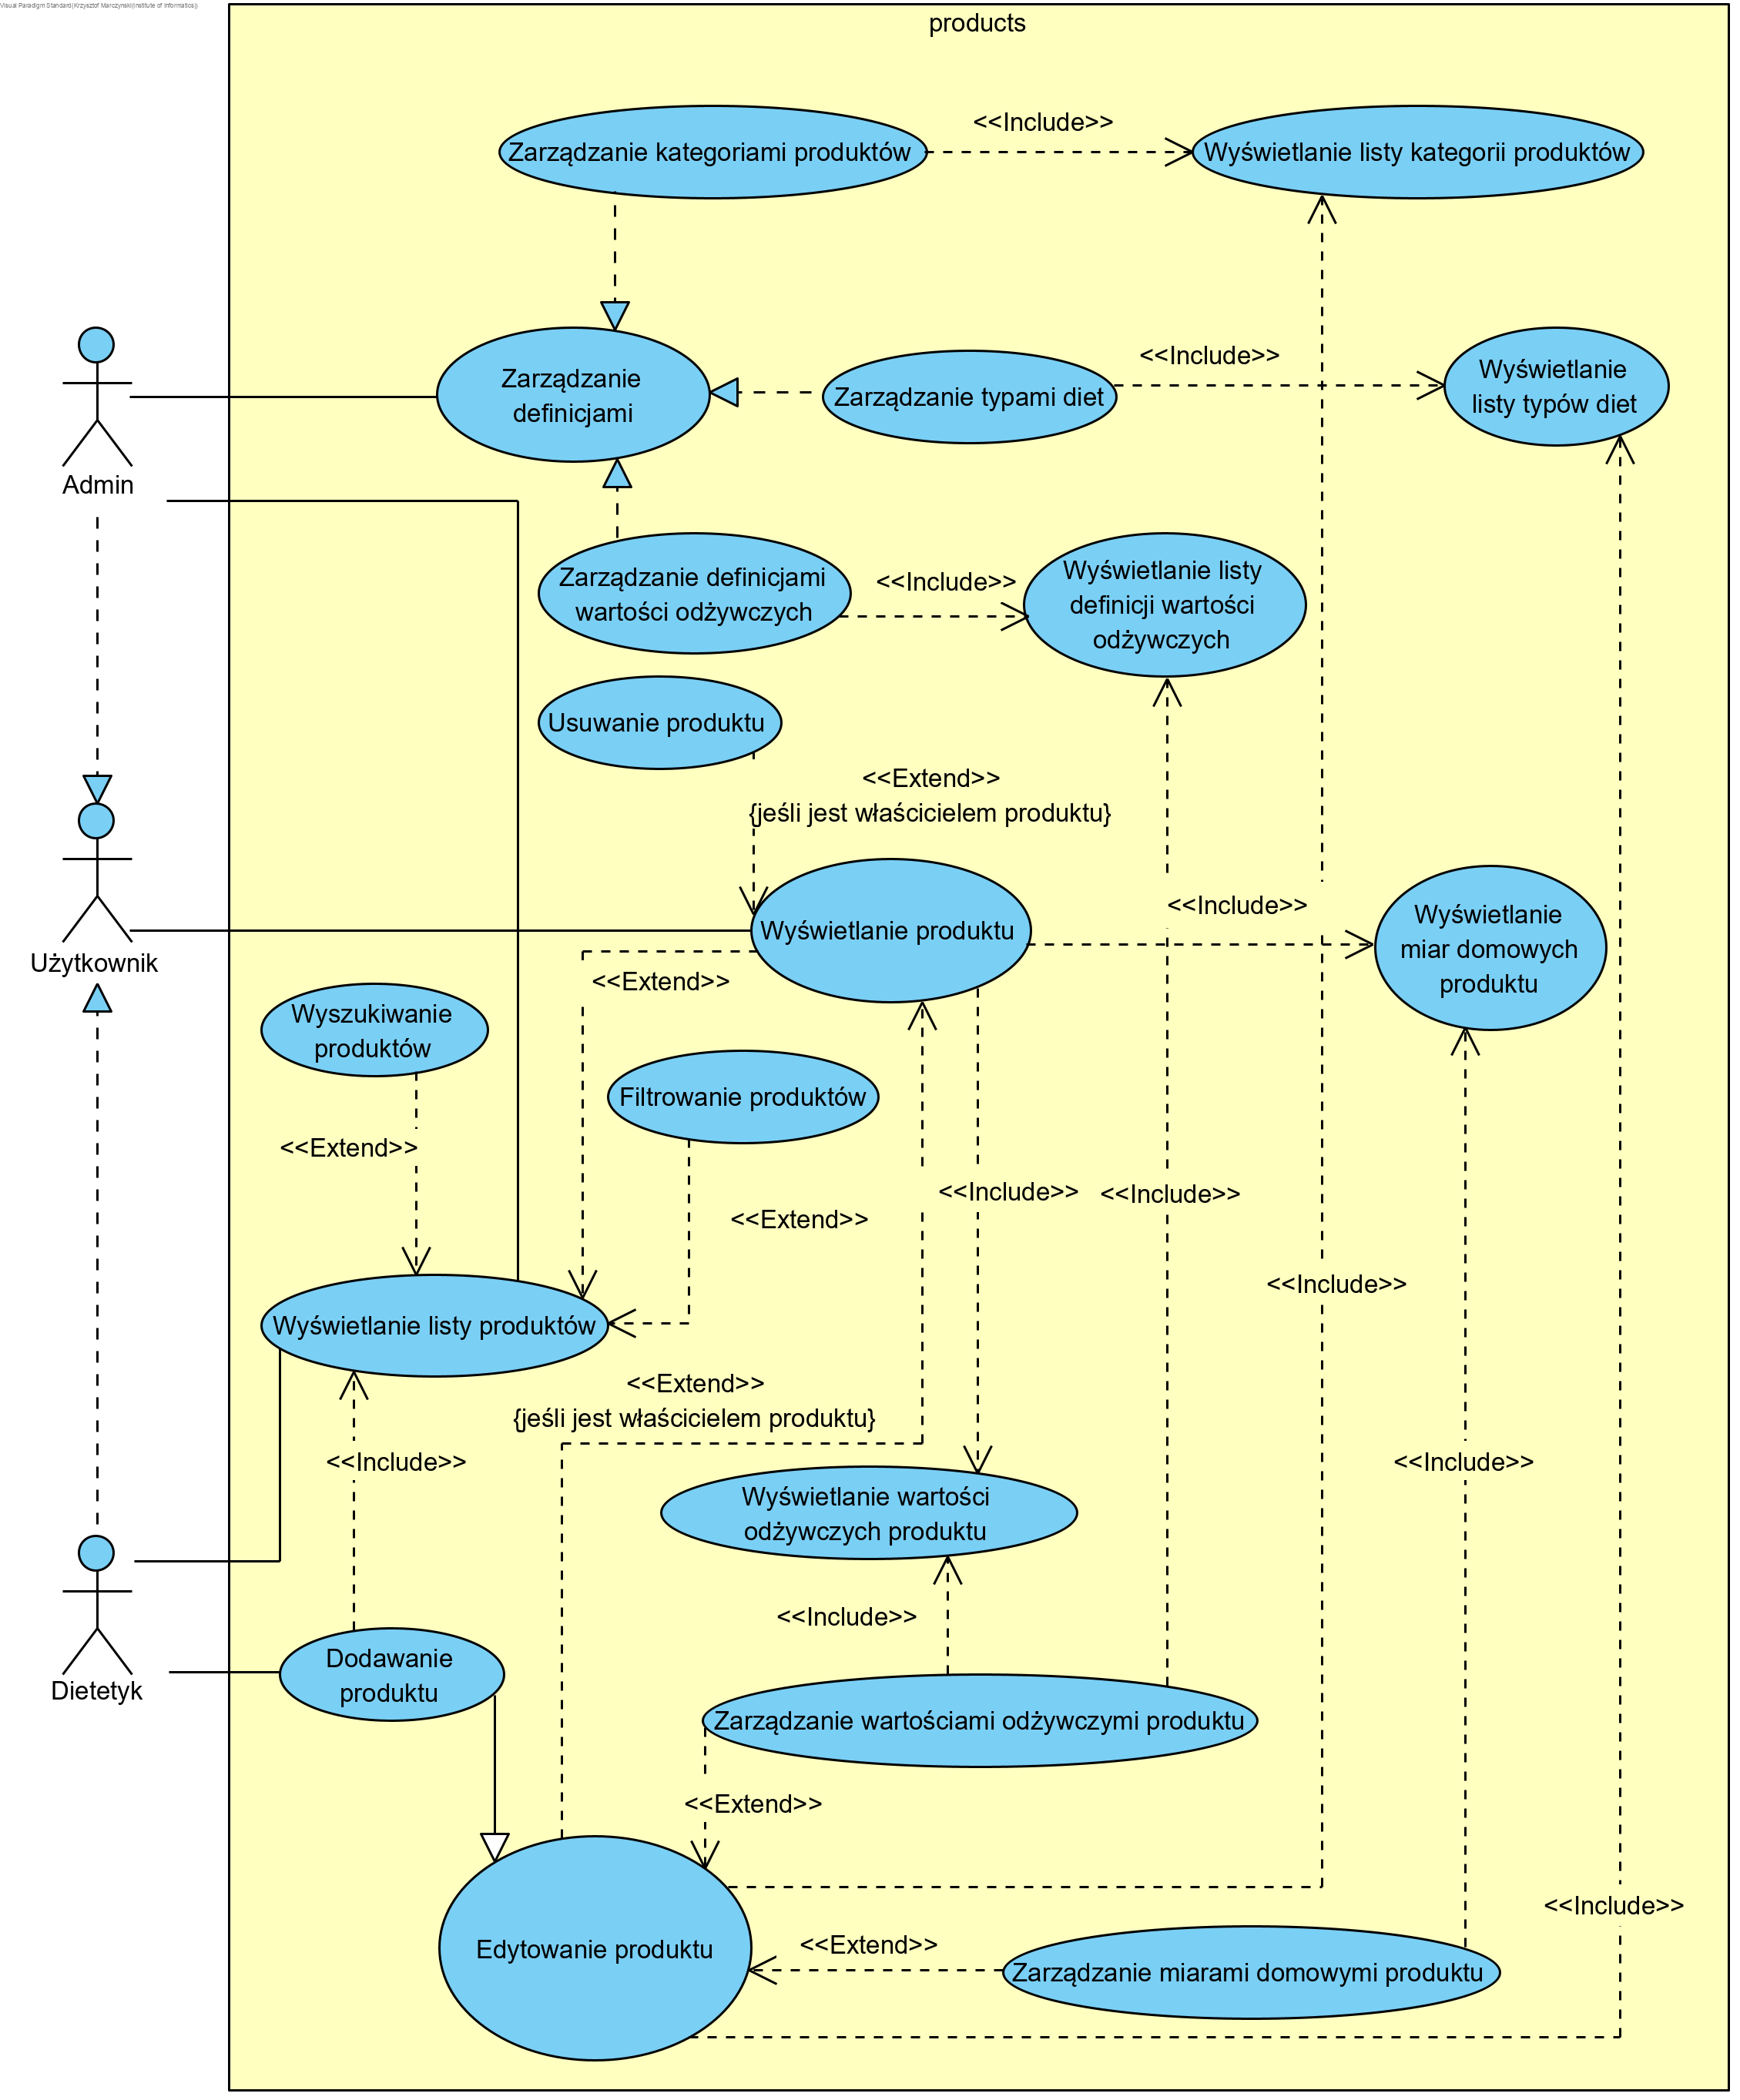
\includegraphics[scale=0.55]{../uml/use_case_diagrams/products.png}
        \caption{Produkty - diagram przypadków użycia (opr.wł).}\label{rysunek:use-case-diagram-products}
    \end{figure}
\end{minipage}

\begin{minipage}{\textwidth}
    \begin{figure}[H]
        \centering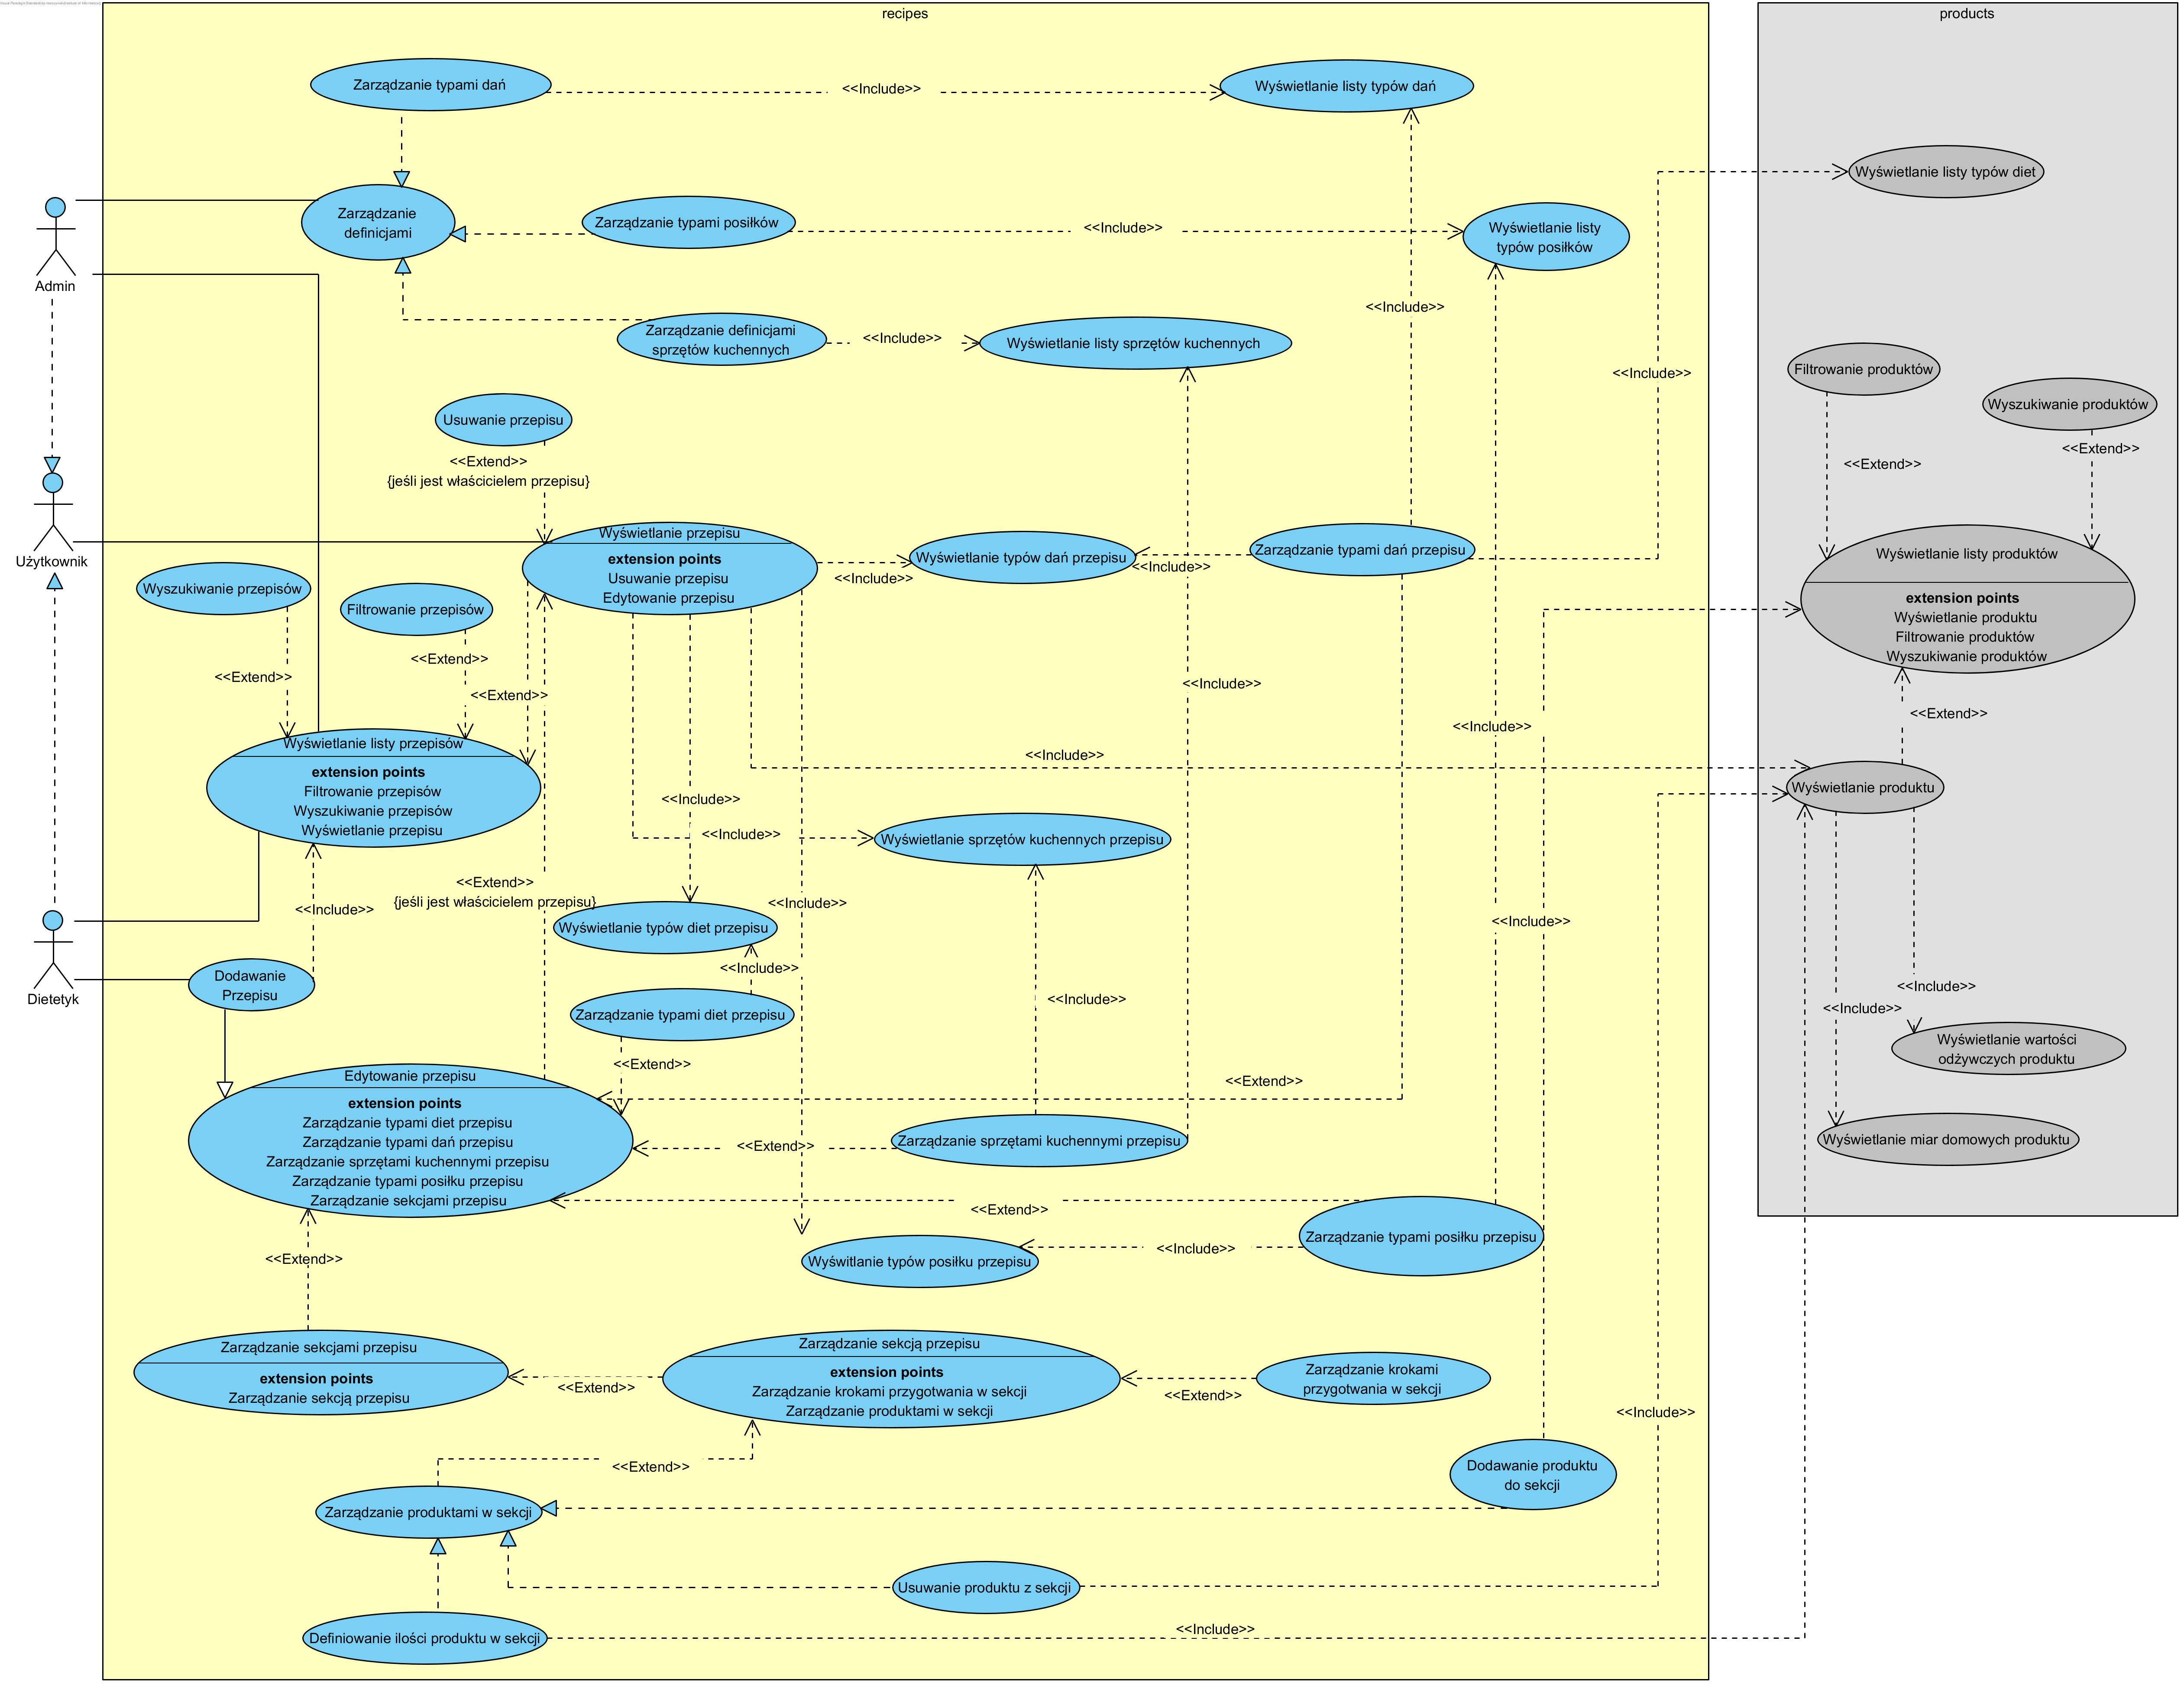
\includegraphics[scale=0.55]{../uml/use_case_diagrams/recipes.png}
        \caption{Przepisy - diagram przypadków użycia (opr.wł).}\label{rysunek:use-case-diagram-recipes}
    \end{figure}
\end{minipage}

\begin{minipage}{\textwidth}
    \begin{figure}[H]
        \centering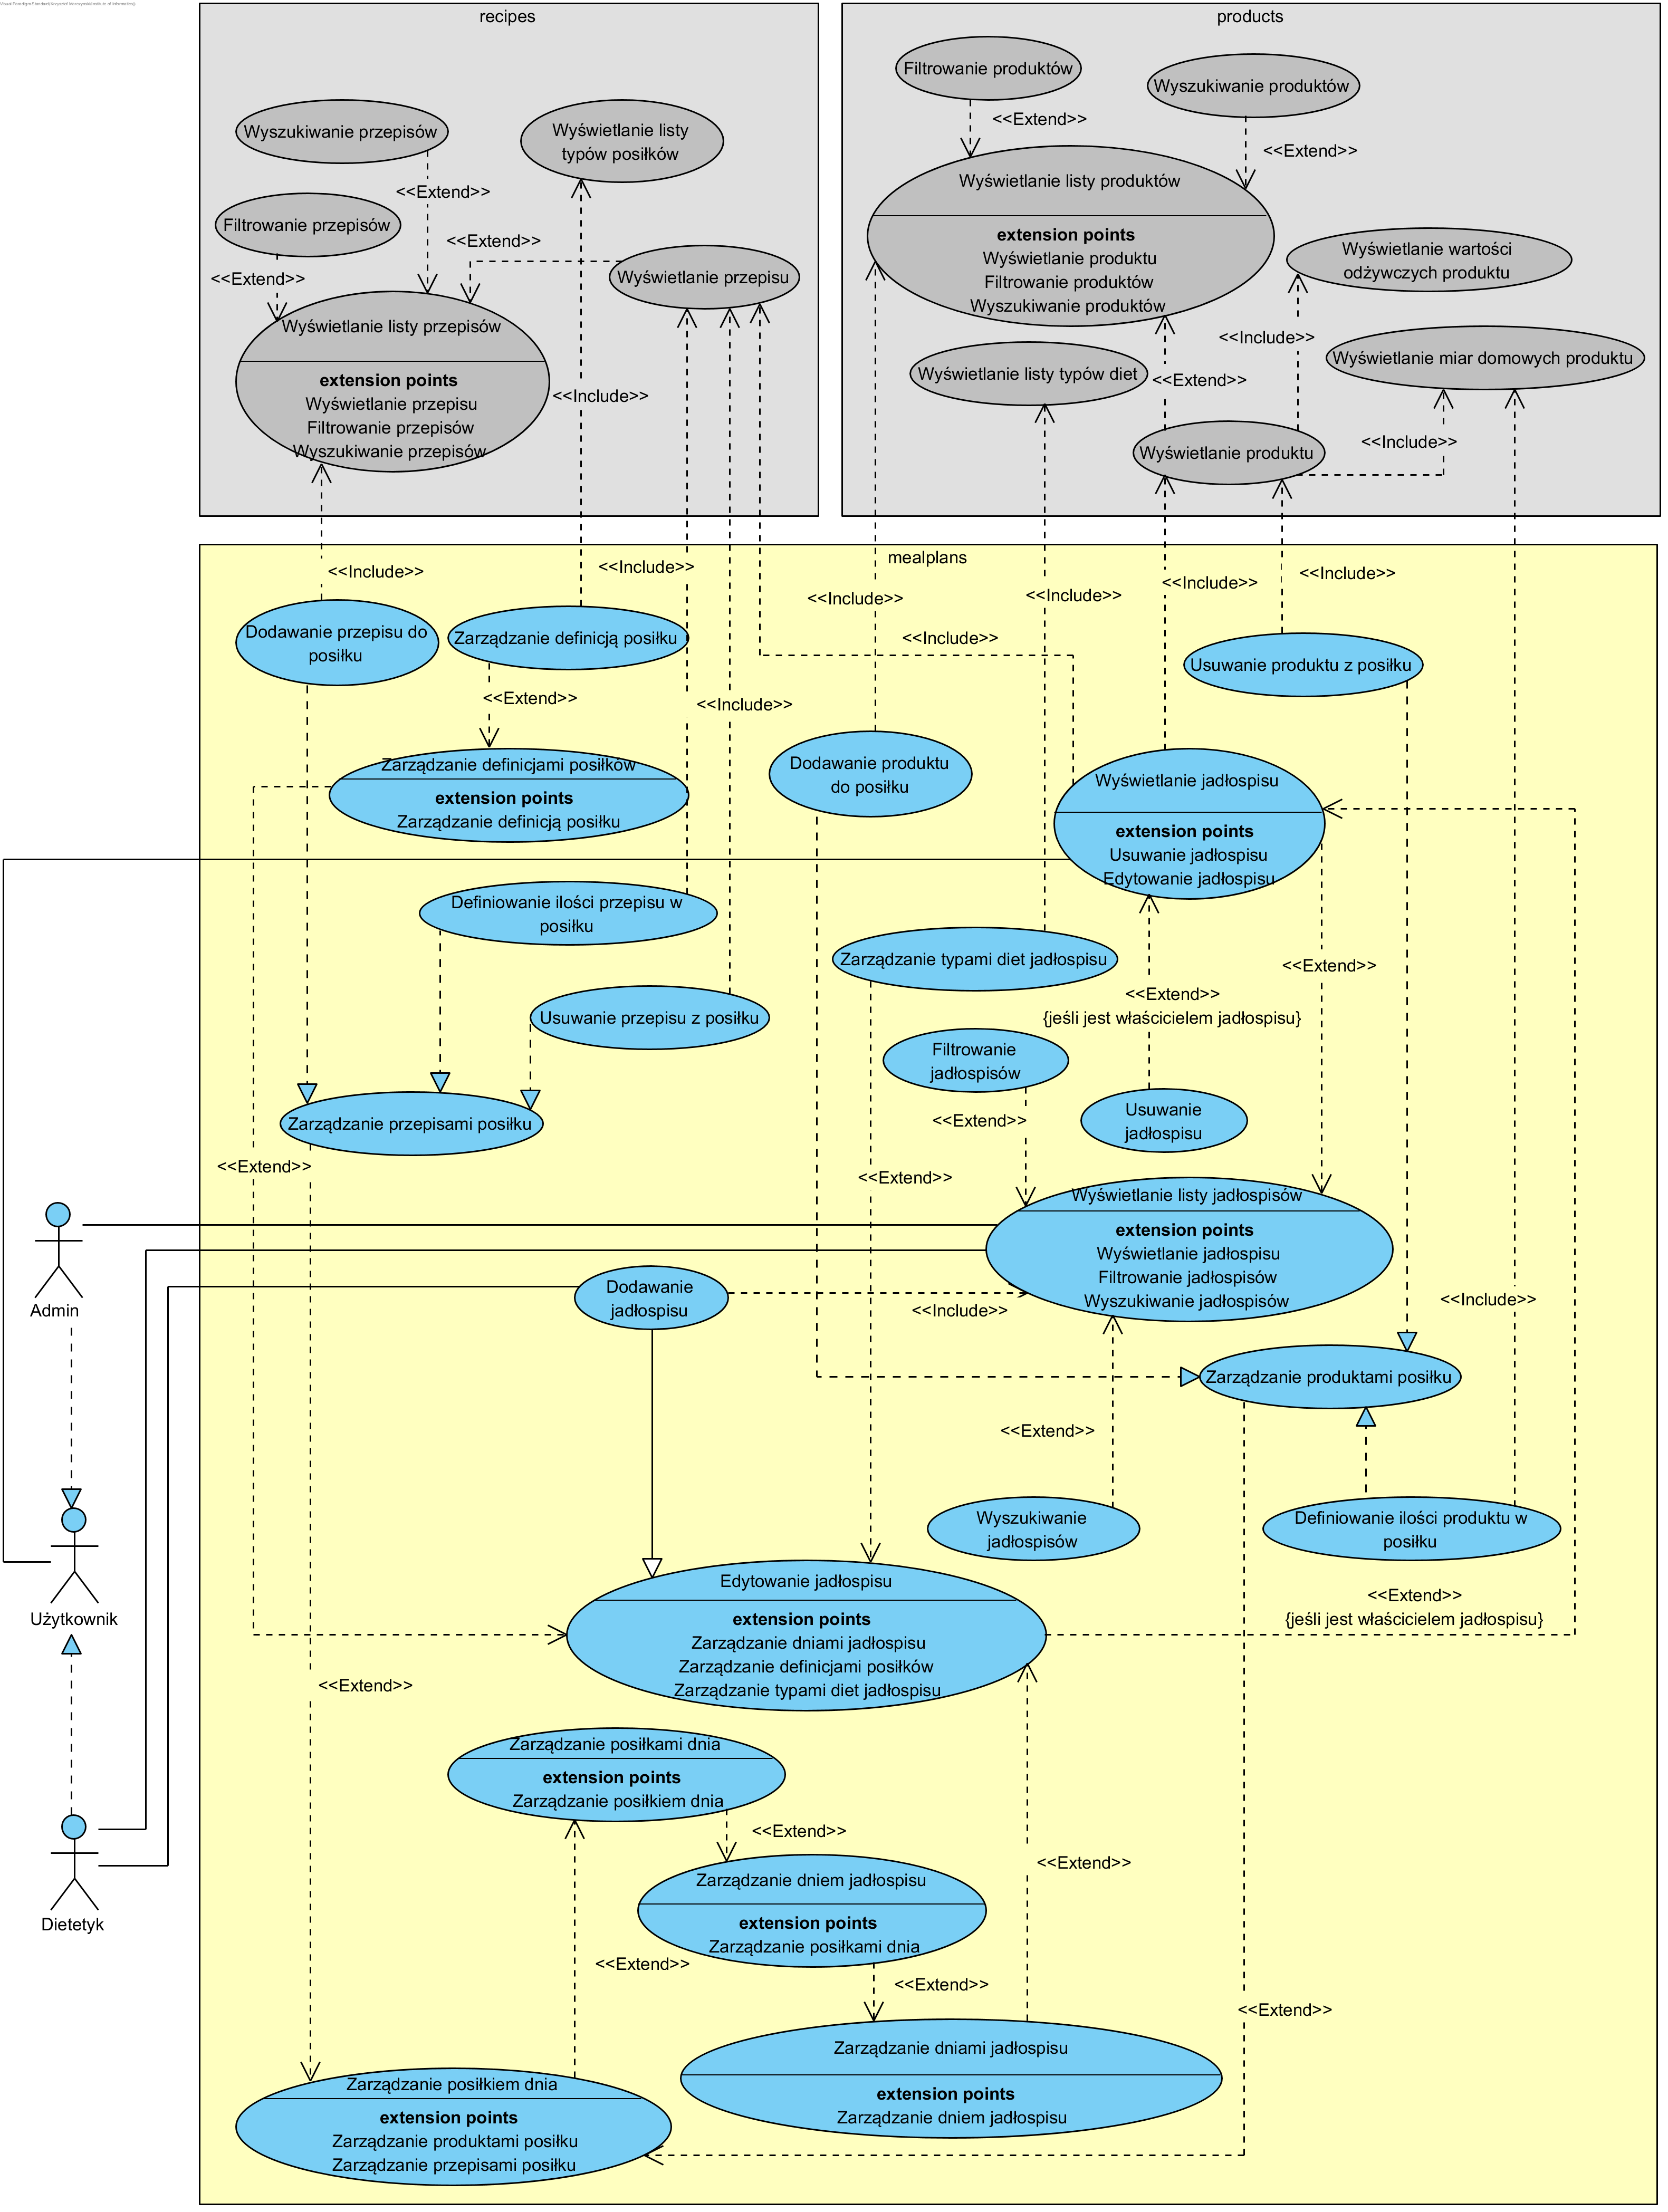
\includegraphics[scale=0.55]{../uml/use_case_diagrams/mealplans.png}
        \caption{Jadłospisy - diagram przypadków użycia (opr.wł).}\label{rysunek:use-case-diagram-mealplans}
    \end{figure}
\end{minipage}

\begin{minipage}{\textwidth}
    \begin{figure}[H]
        \centering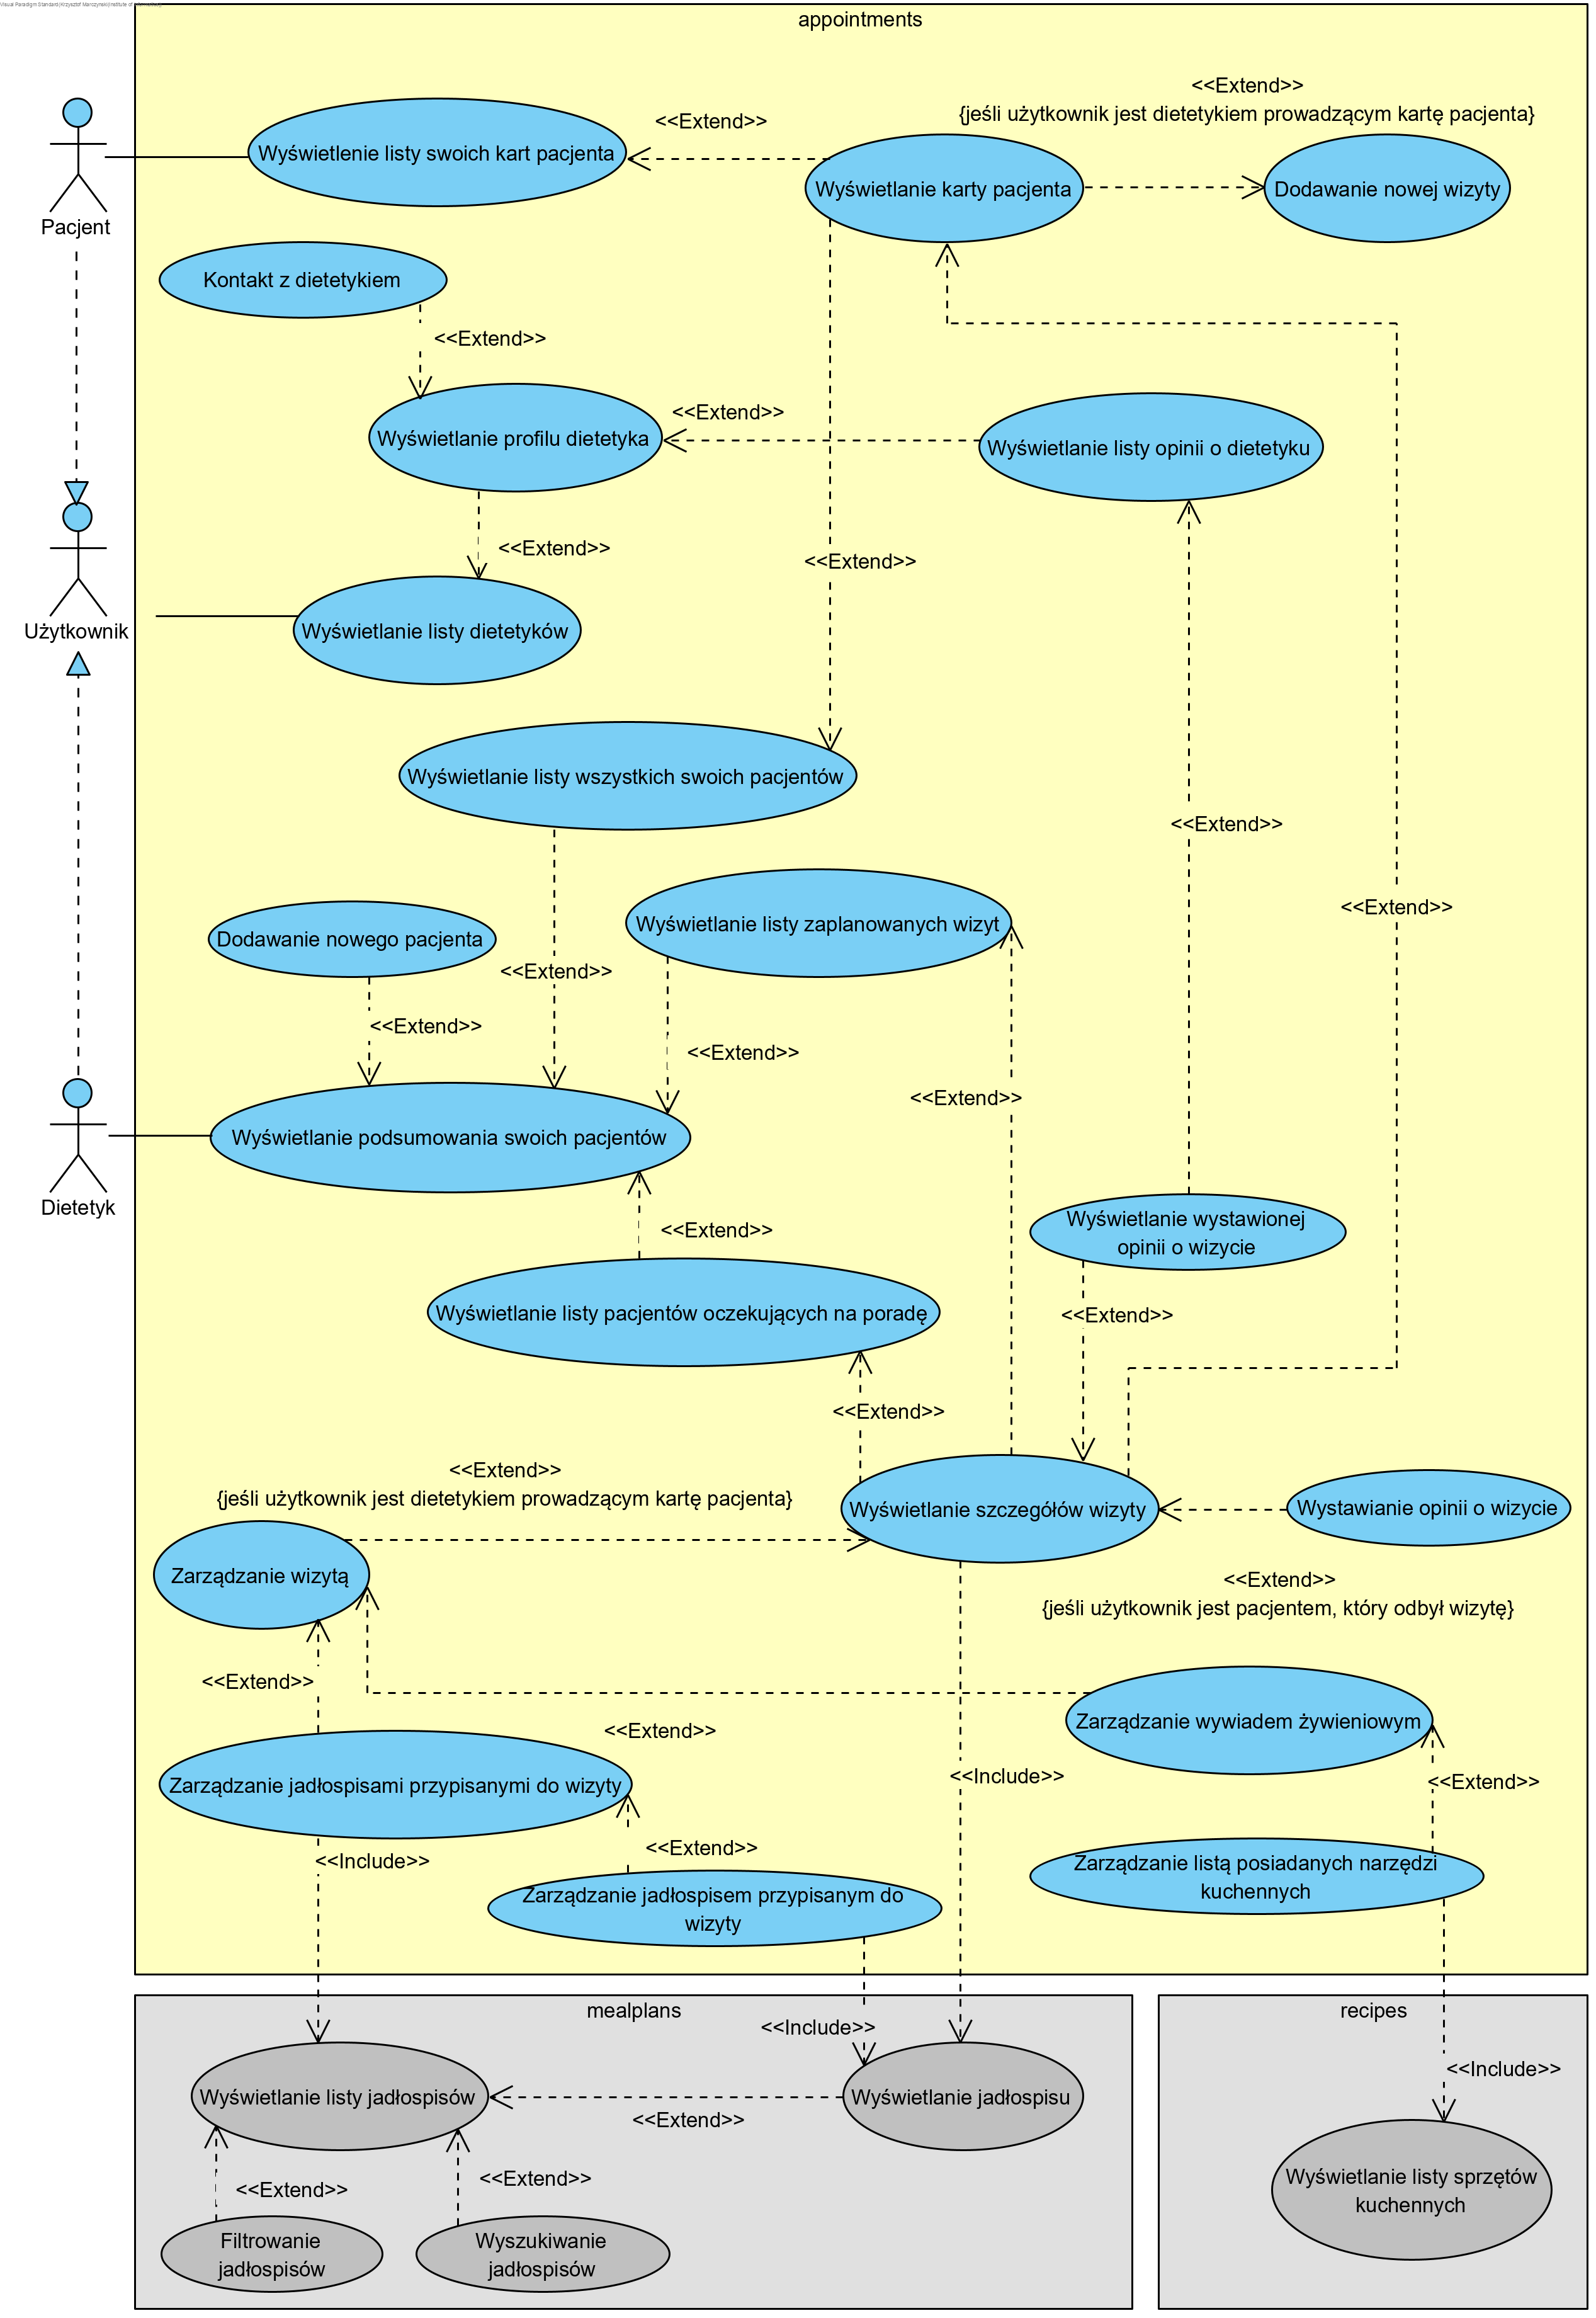
\includegraphics[scale=0.55]{../uml/use_case_diagrams/appointments.png}
        \caption{Wizyty - diagram przypadków użycia (opr.wł).}\label{rysunek:use-case-diagram-appointments}
    \end{figure}
\end{minipage}

\section{Prototyp interfejsu}
\todo{mockupy}
\begin{minipage}{\textwidth}
    \begin{figure}[H]
        \centering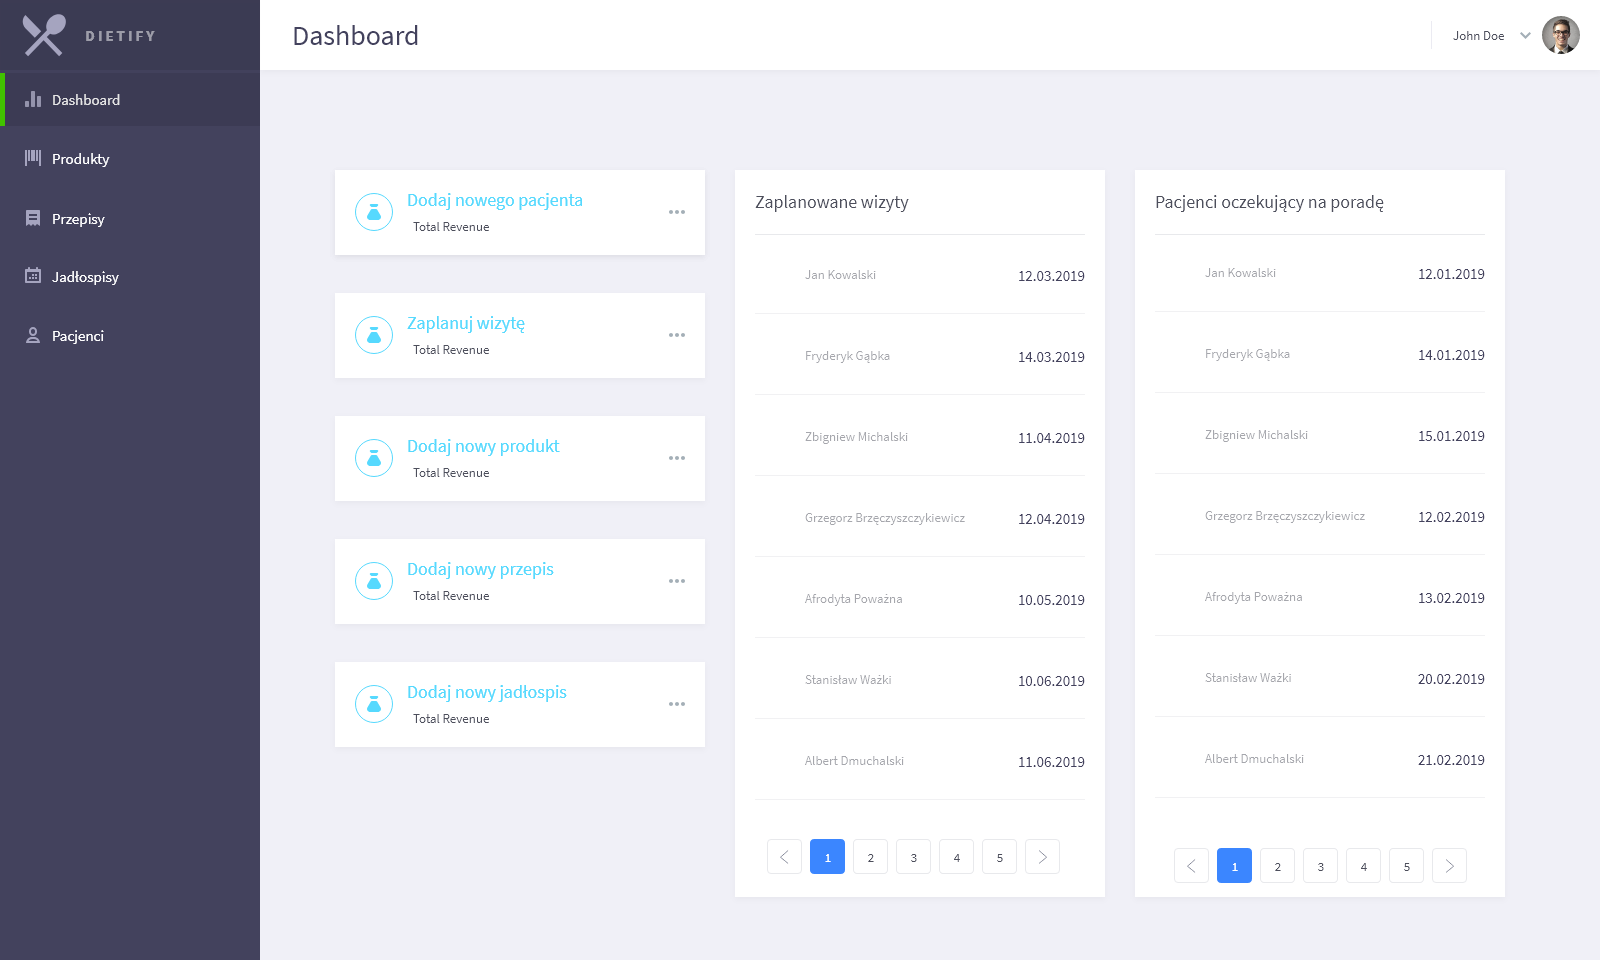
\includegraphics[width=0.9\textwidth]{img/mockups/mockup1.png}
        \caption{Mockup1 (opr.wł).}\label{rysunek:mockup1}
    \end{figure}
\end{minipage}

\begin{minipage}{\textwidth}
    \begin{figure}[H]
        \centering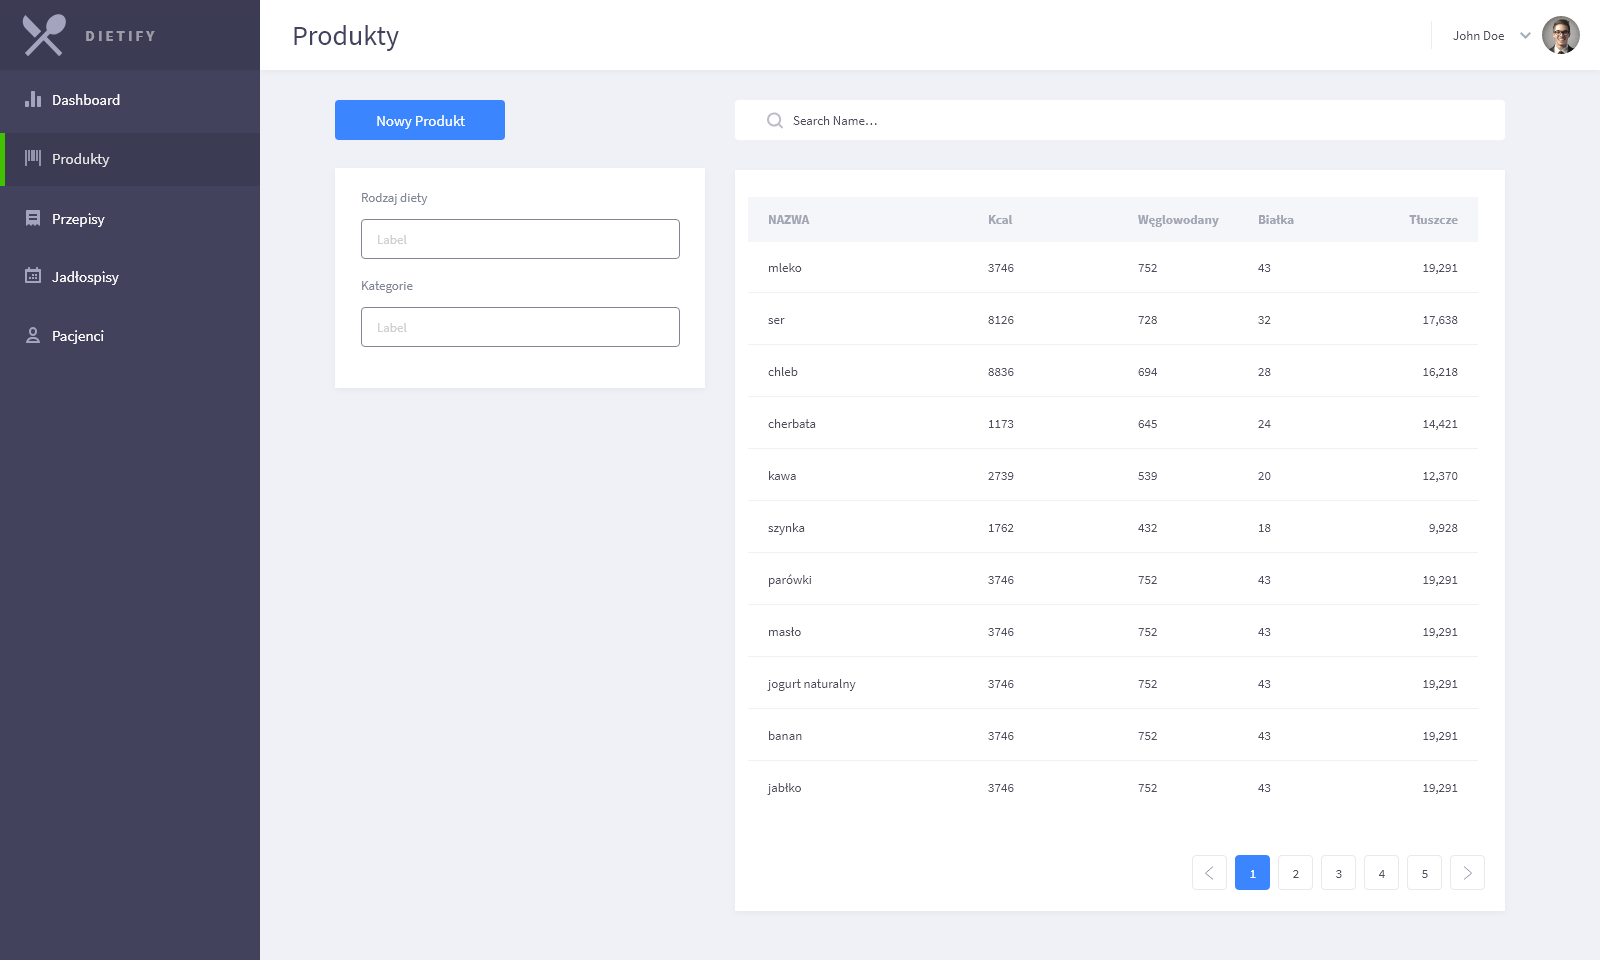
\includegraphics[width=0.9\textwidth]{img/mockups/mockup2.png}
        \caption{Mockup2 (opr.wł).}\label{rysunek:mockup2}
    \end{figure}
\end{minipage}

\begin{minipage}{\textwidth}
    \begin{figure}[H]
        \centering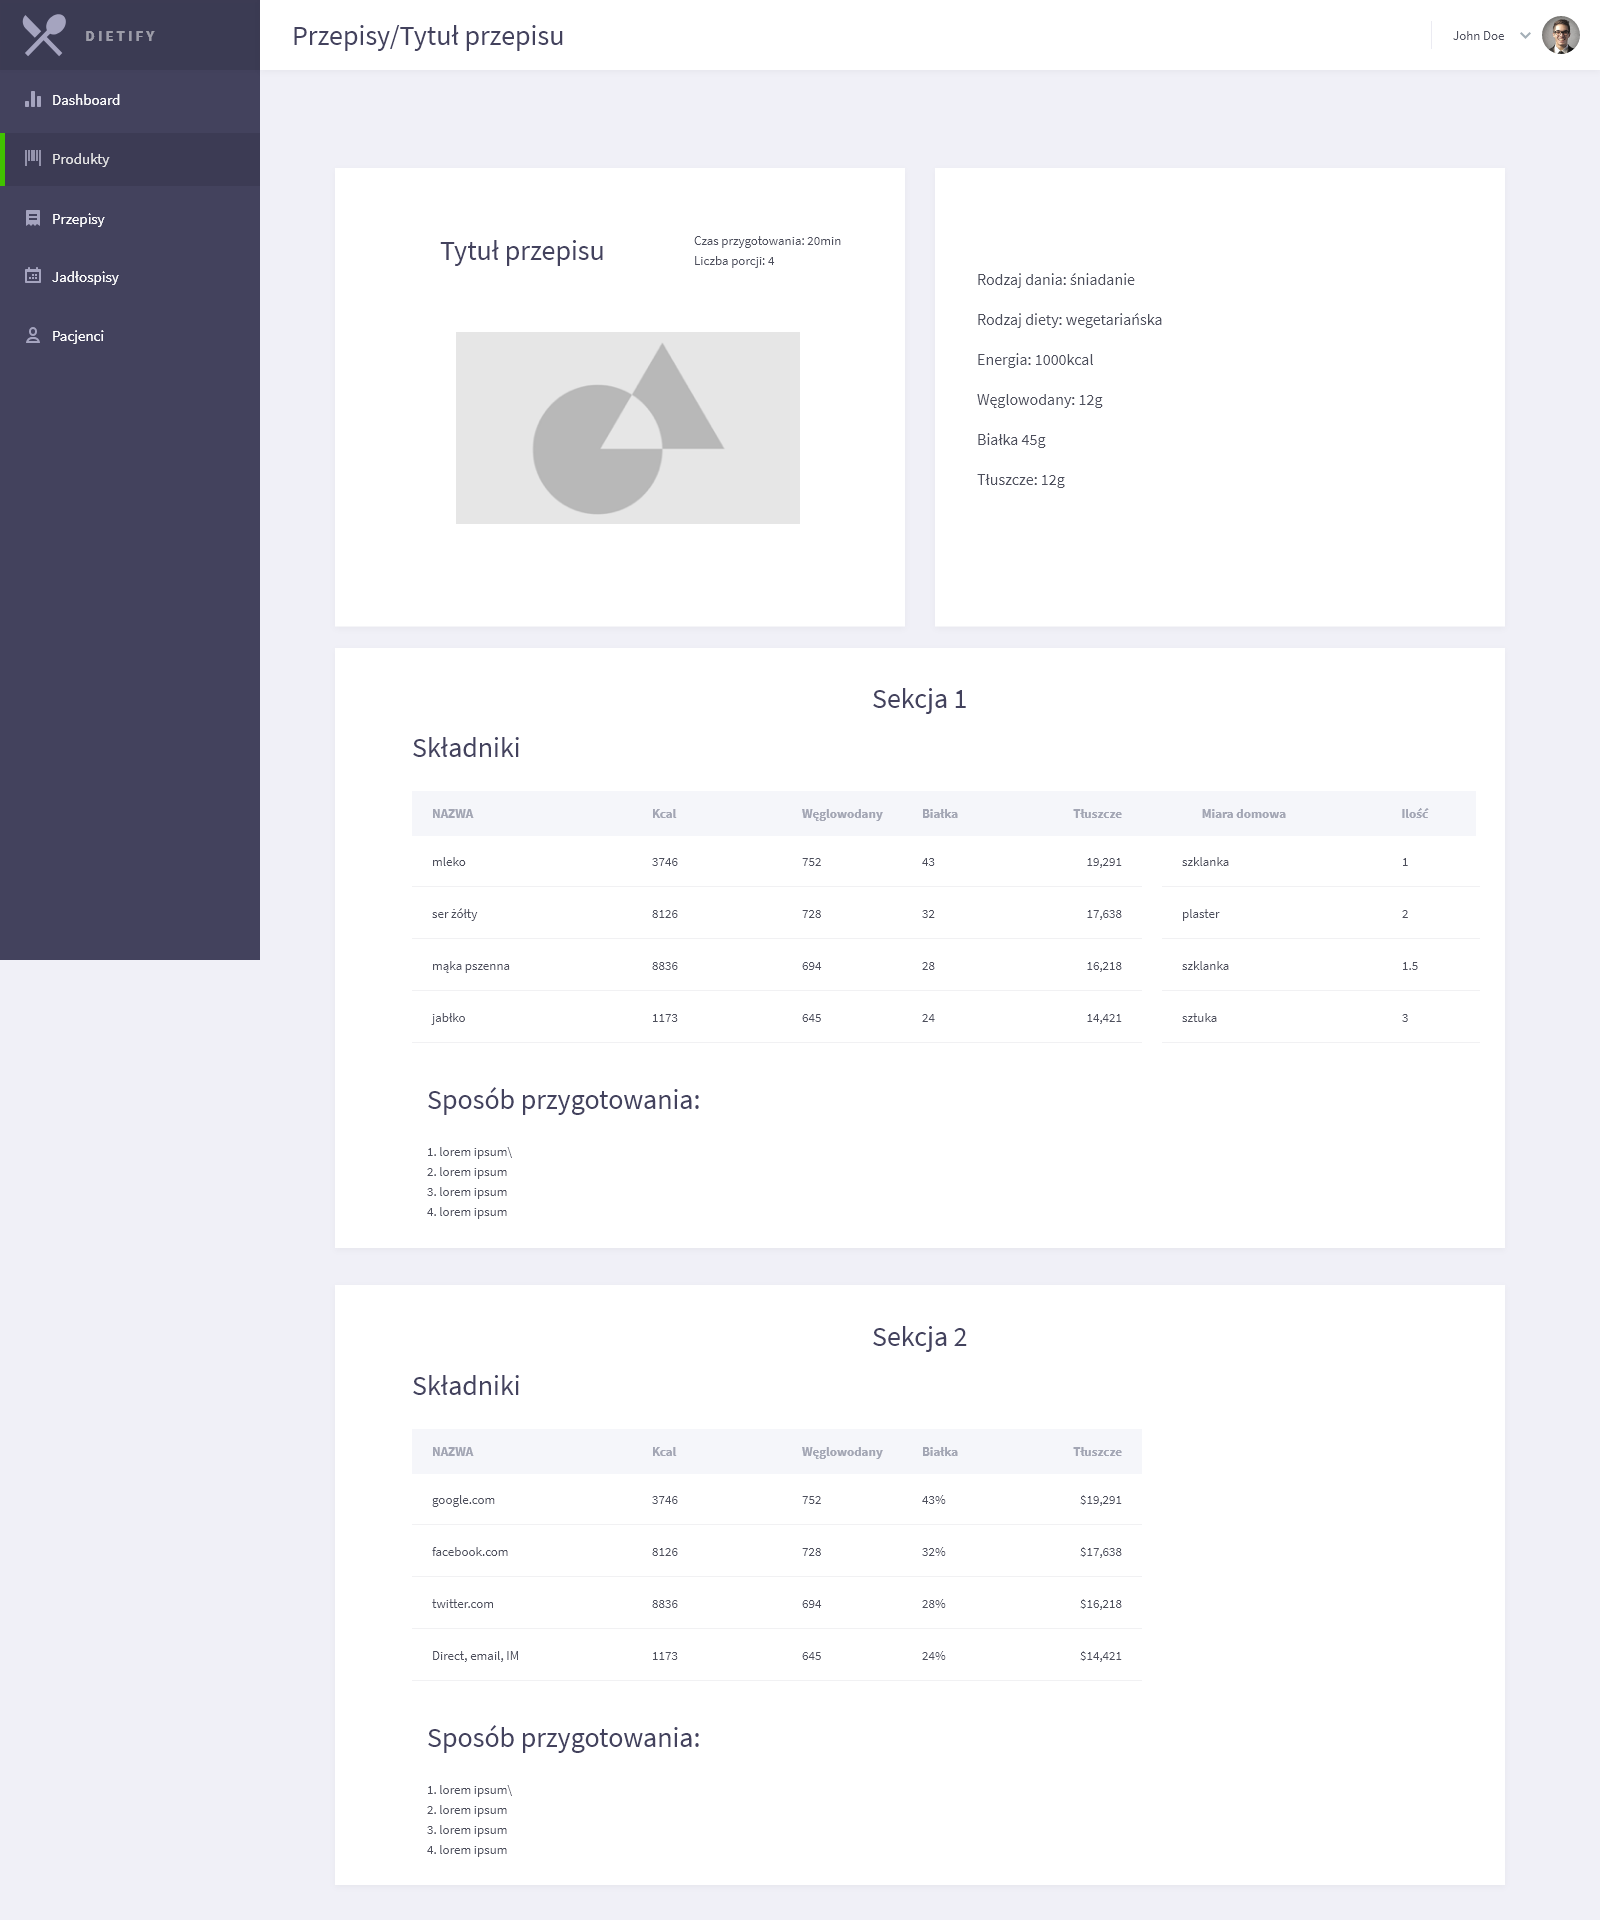
\includegraphics[width=0.9\textwidth]{img/mockups/mockup3.png}
        \caption{Mockup3 (opr.wł).}\label{rysunek:mockup3}
    \end{figure}
\end{minipage}

\begin{minipage}{\textwidth}
    \begin{figure}[H]
        \centering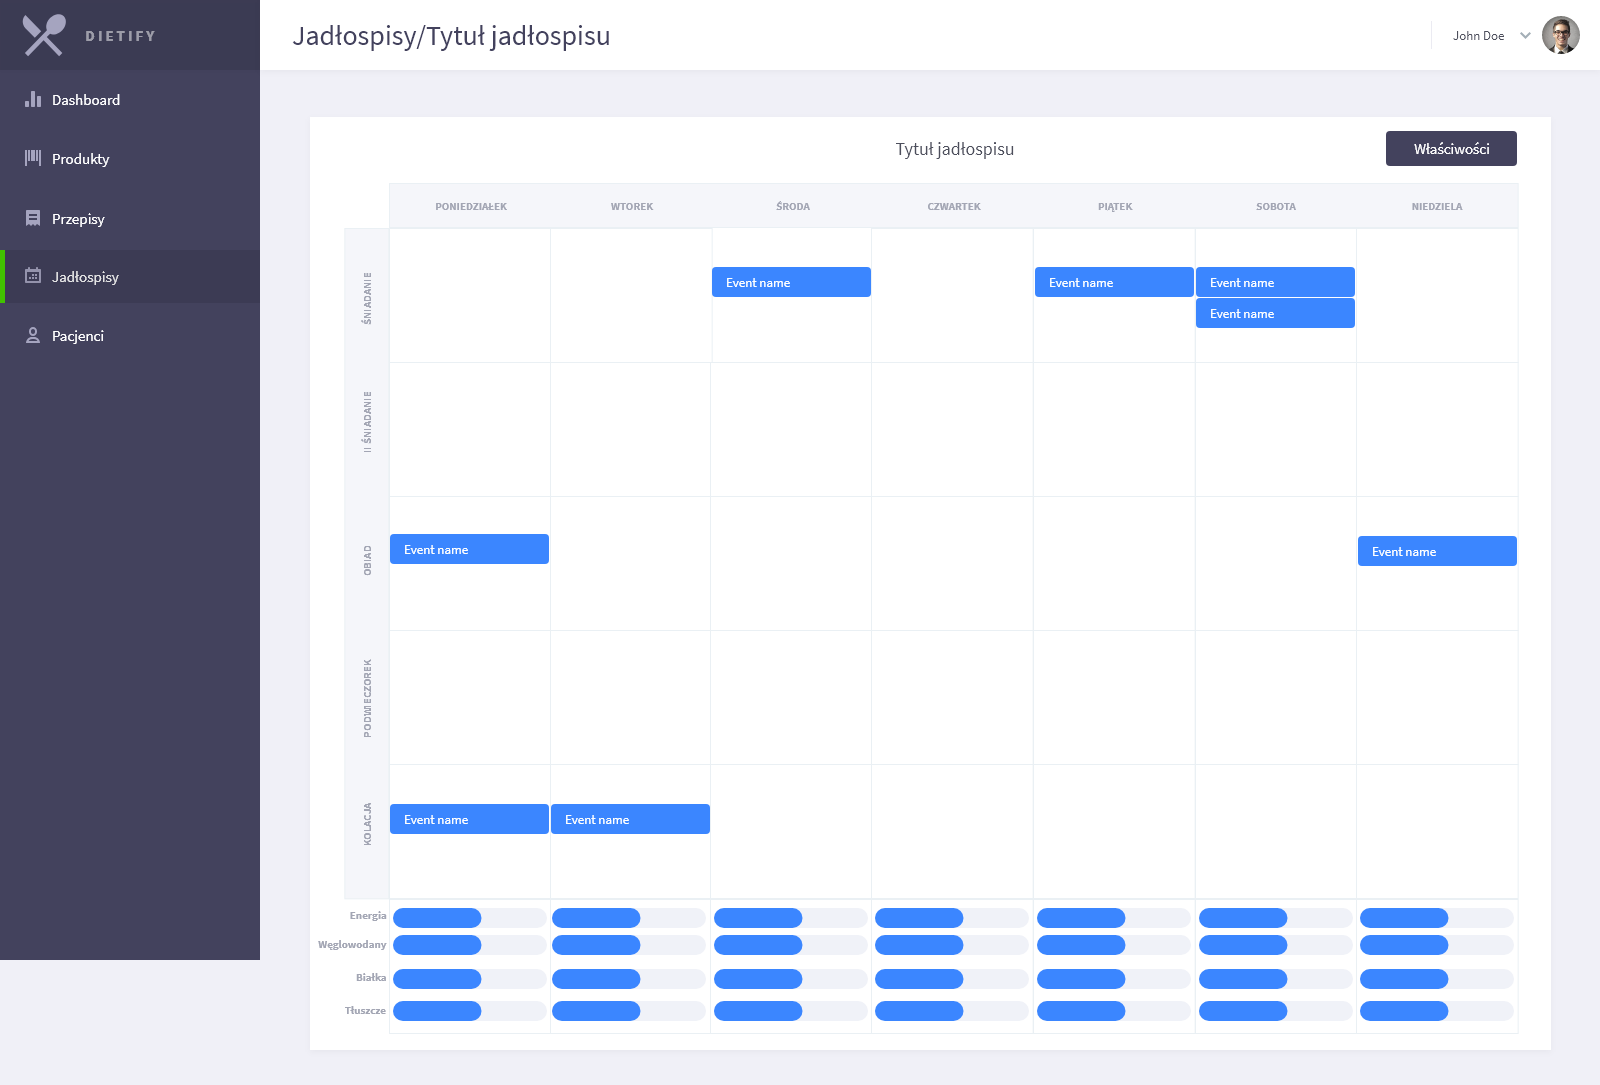
\includegraphics[width=0.9\textwidth]{img/mockups/mockup4.png}
        \caption{Mockup4 (opr.wł).}\label{rysunek:mockup4}
    \end{figure}
\end{minipage}

\begin{minipage}{\textwidth}
    \begin{figure}[H]
        \centering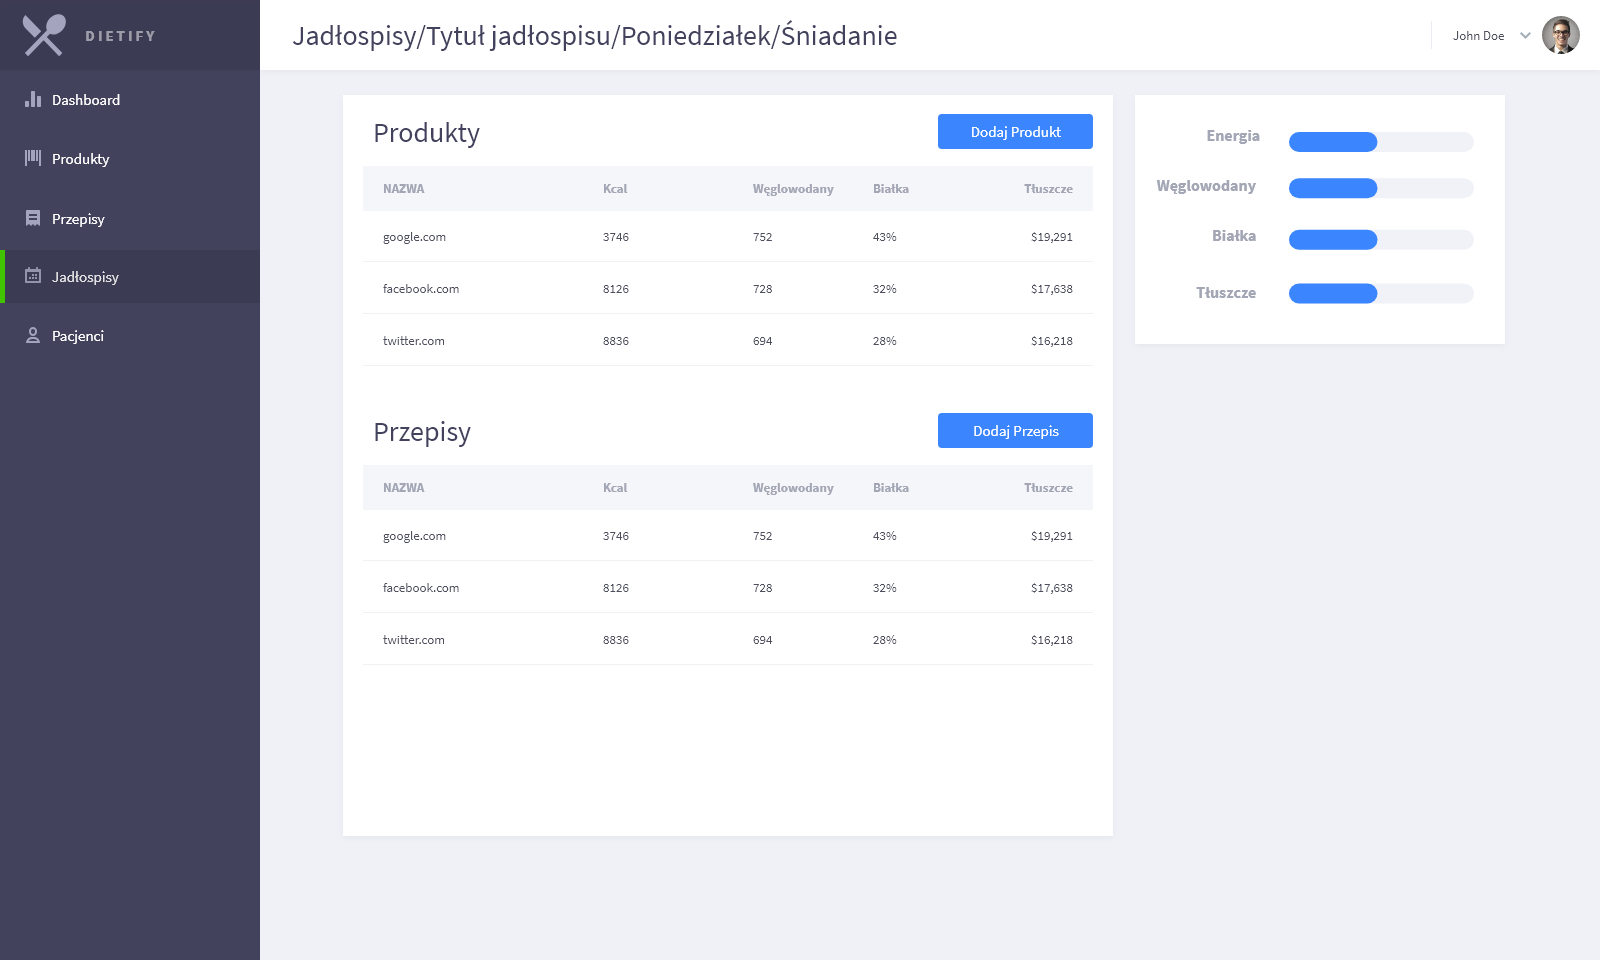
\includegraphics[width=0.9\textwidth]{img/mockups/mockup5.png}
        \caption{Mockup5 (opr.wł).}\label{rysunek:mockup5}
    \end{figure}
\end{minipage}

\begin{minipage}{\textwidth}
    \begin{figure}[H]
        \centering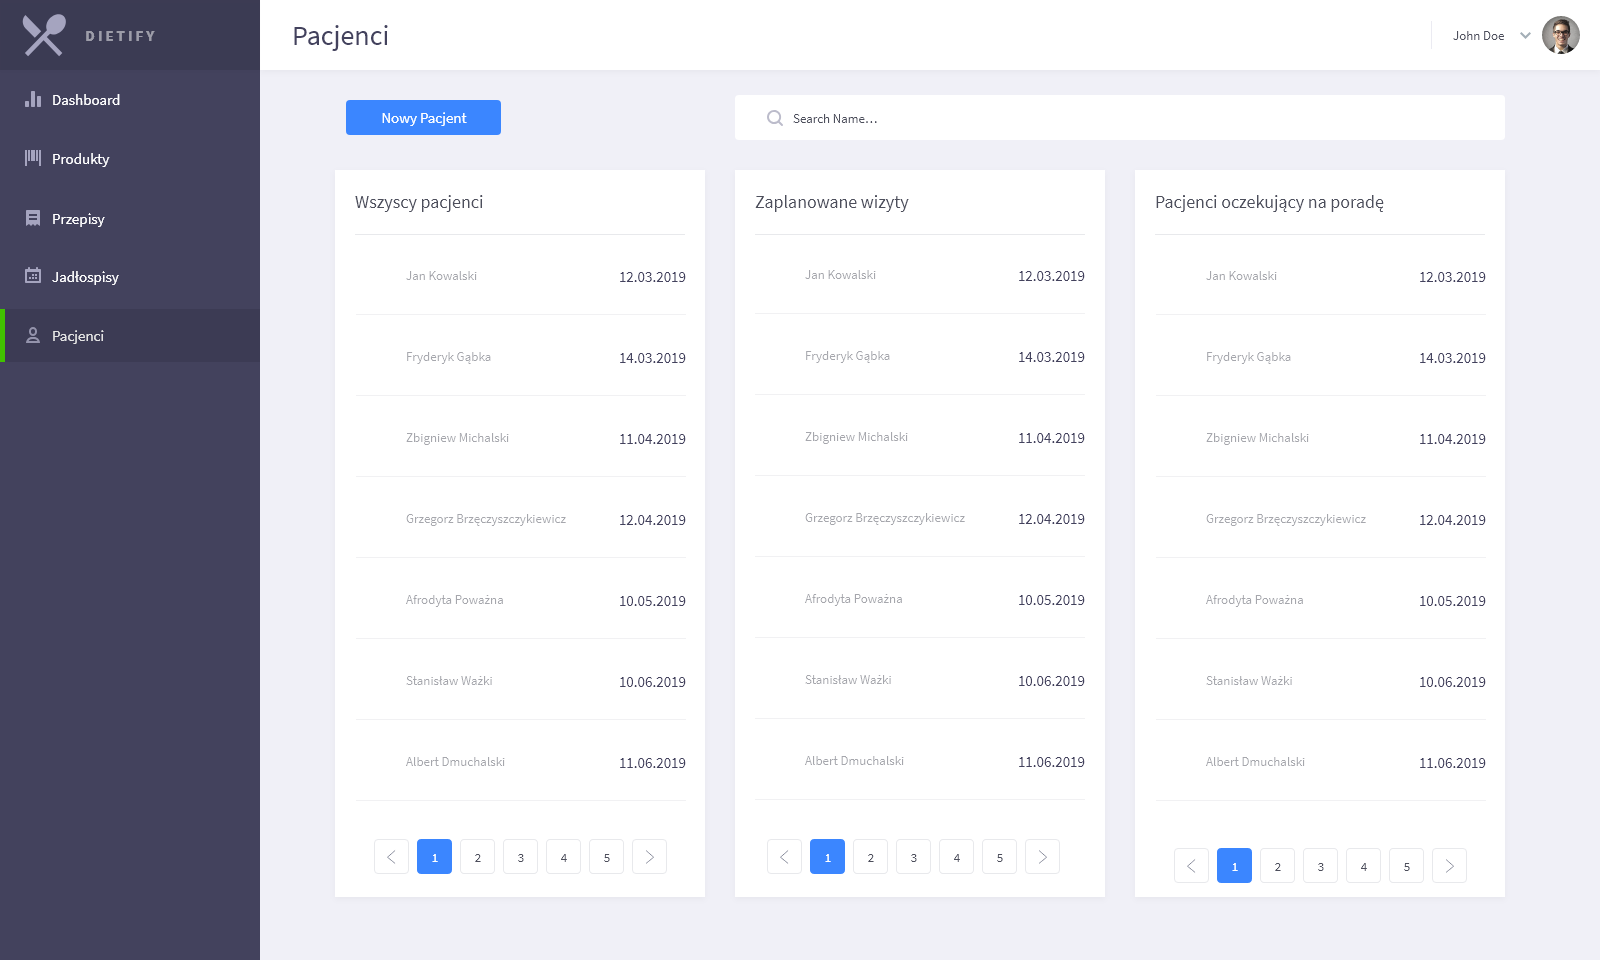
\includegraphics[width=0.9\textwidth]{img/mockups/mockup6.png}
        \caption{Mockup6 (opr.wł).}\label{rysunek:mockup6}
    \end{figure}
\end{minipage}

\begin{minipage}{\textwidth}
    \begin{figure}[H]
        \centering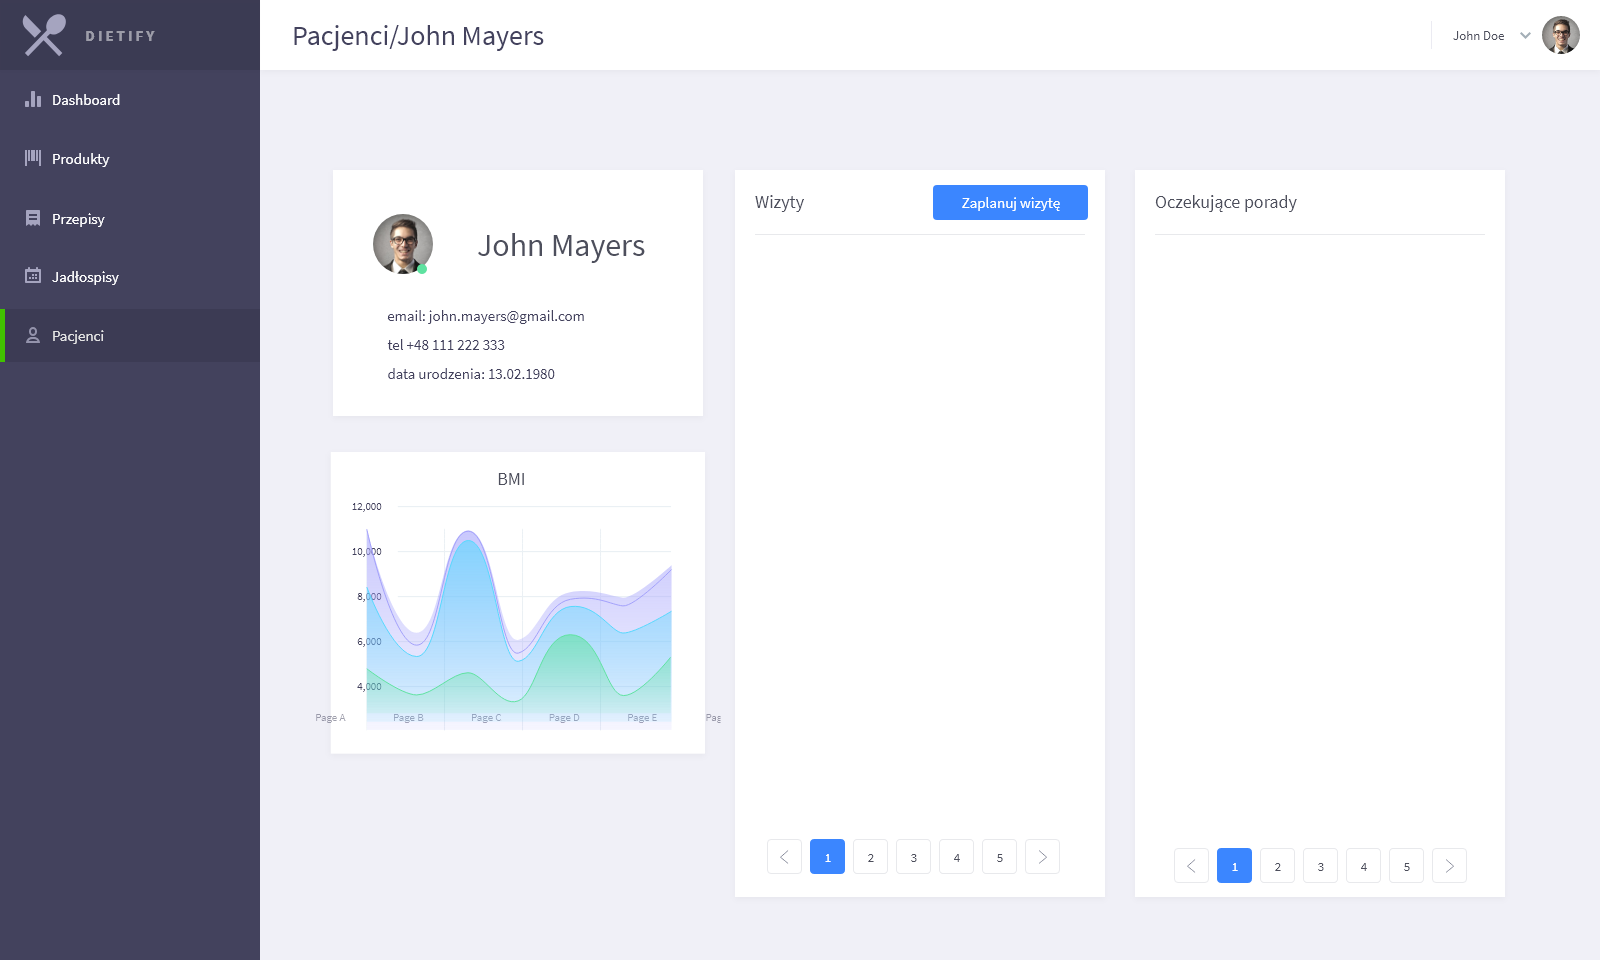
\includegraphics[width=0.9\textwidth]{img/mockups/mockup7.png}
        \caption{Mockup7 (opr.wł).}\label{rysunek:mockup7}
    \end{figure}
\end{minipage}

\begin{minipage}{\textwidth}
    \begin{figure}[H]
        \centering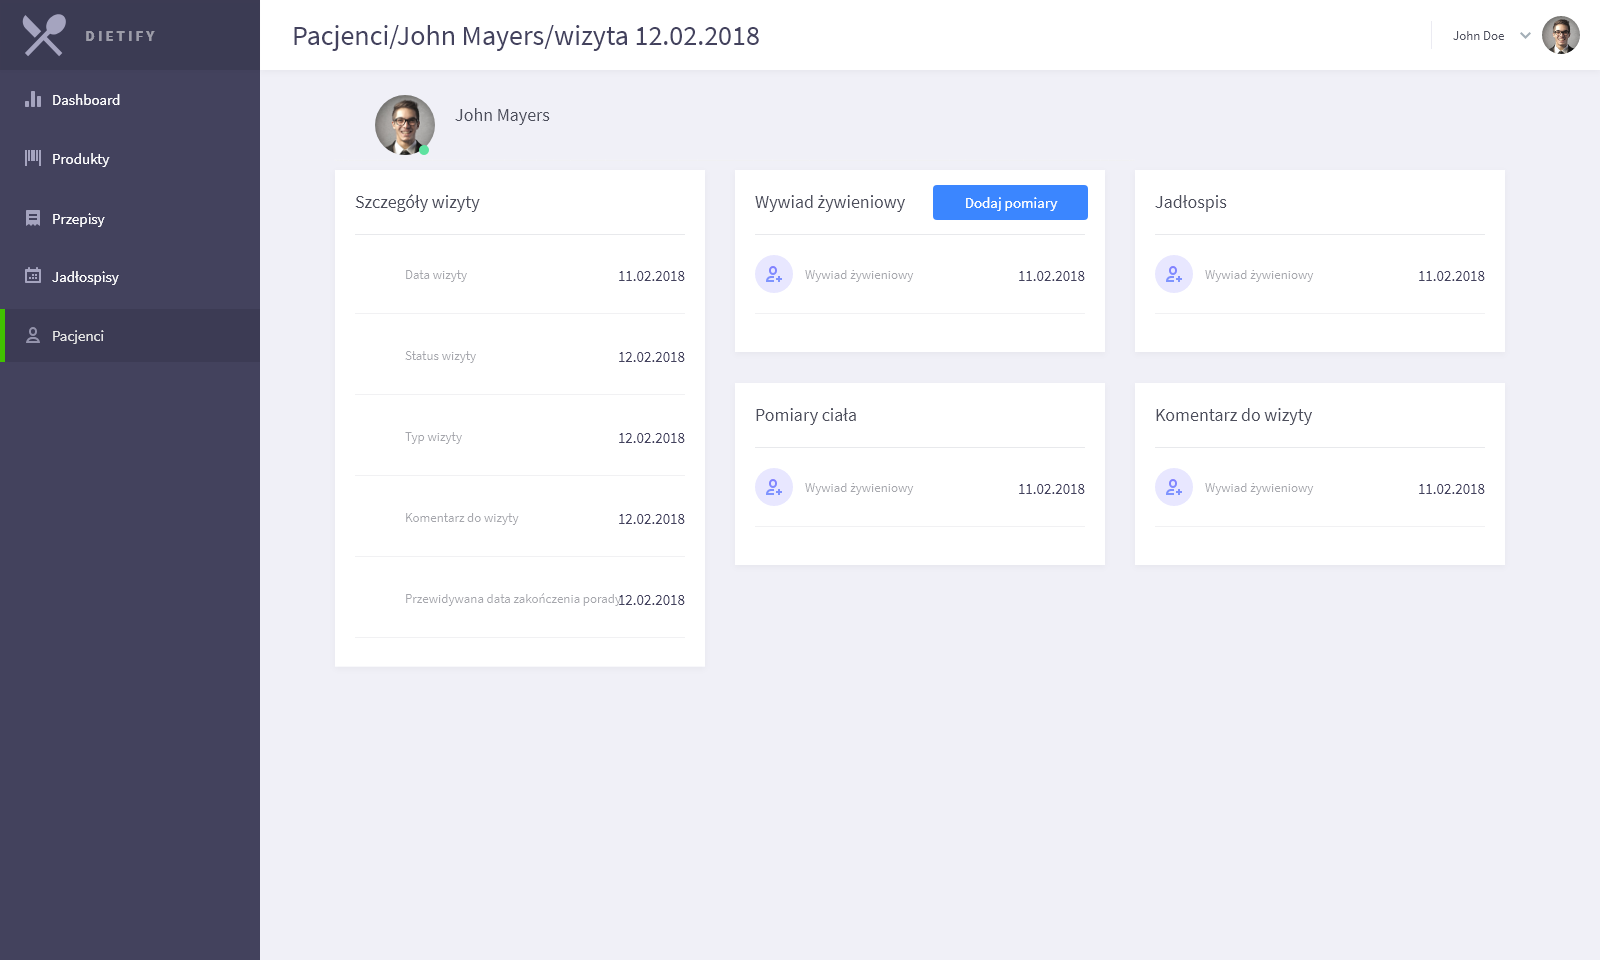
\includegraphics[width=0.9\textwidth]{img/mockups/mockup8.png}
        \caption{Mockup8 (opr.wł).}\label{rysunek:mockup8}
    \end{figure}
\end{minipage}

\begin{minipage}{\textwidth}
    \begin{figure}[H]
        \centering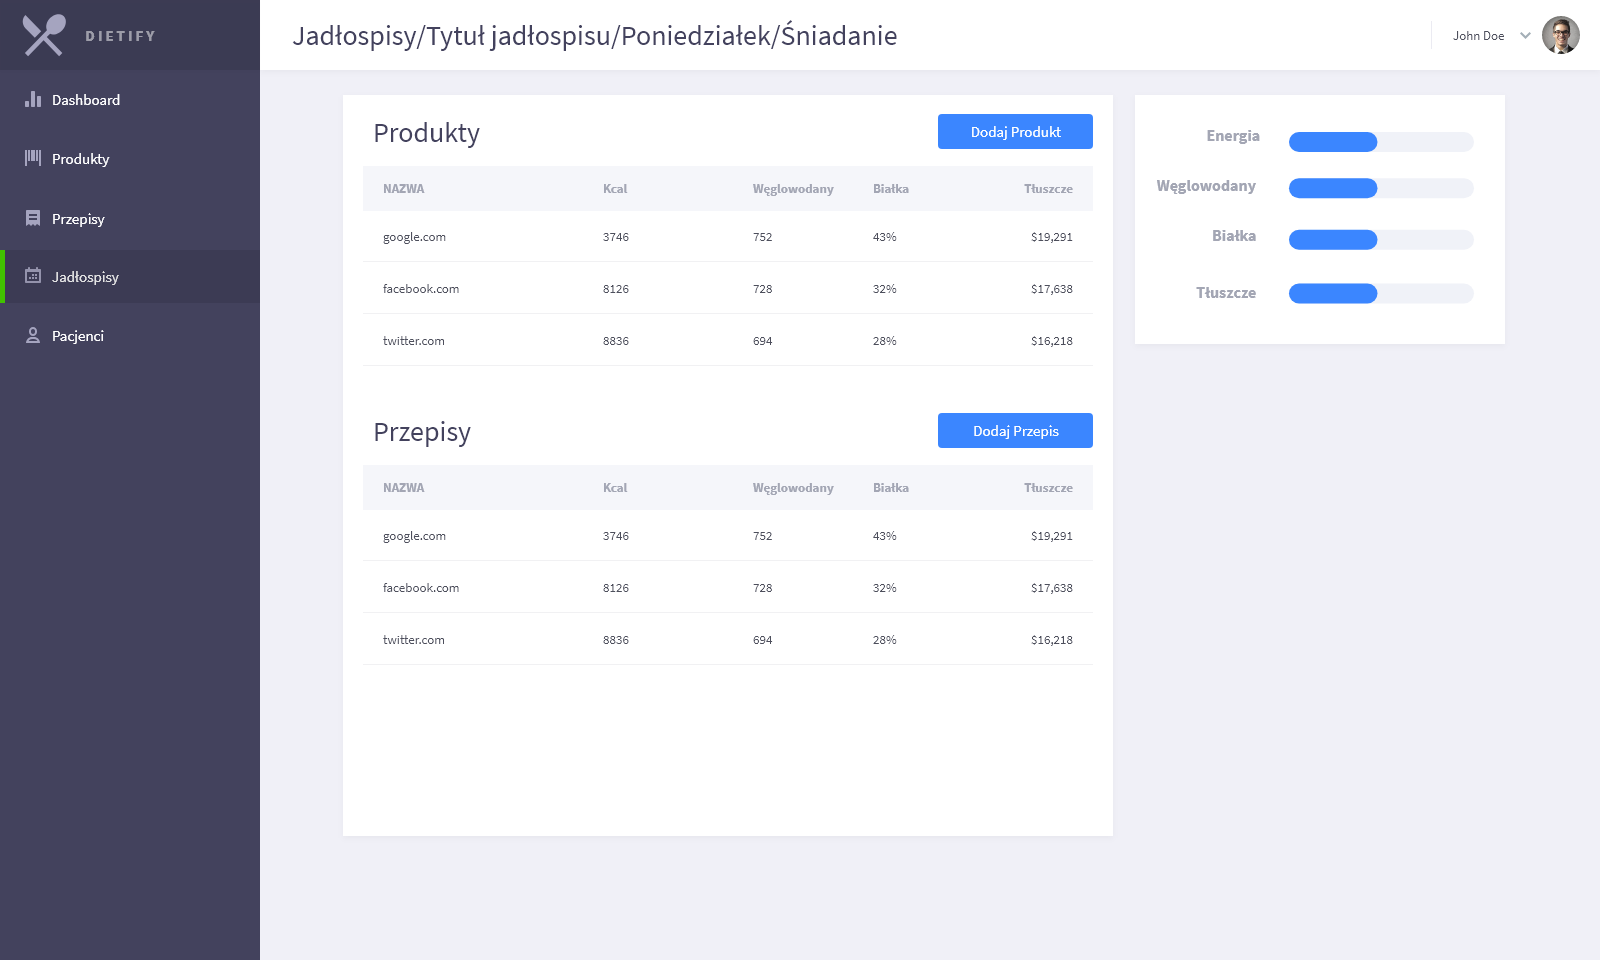
\includegraphics[width=0.9\textwidth]{img/mockups/mockup9.png}
        \caption{Mockup9 (opr.wł).}\label{rysunek:mockup9}
    \end{figure}
\end{minipage}

\begin{minipage}{\textwidth}
    \begin{figure}[H]
        \centering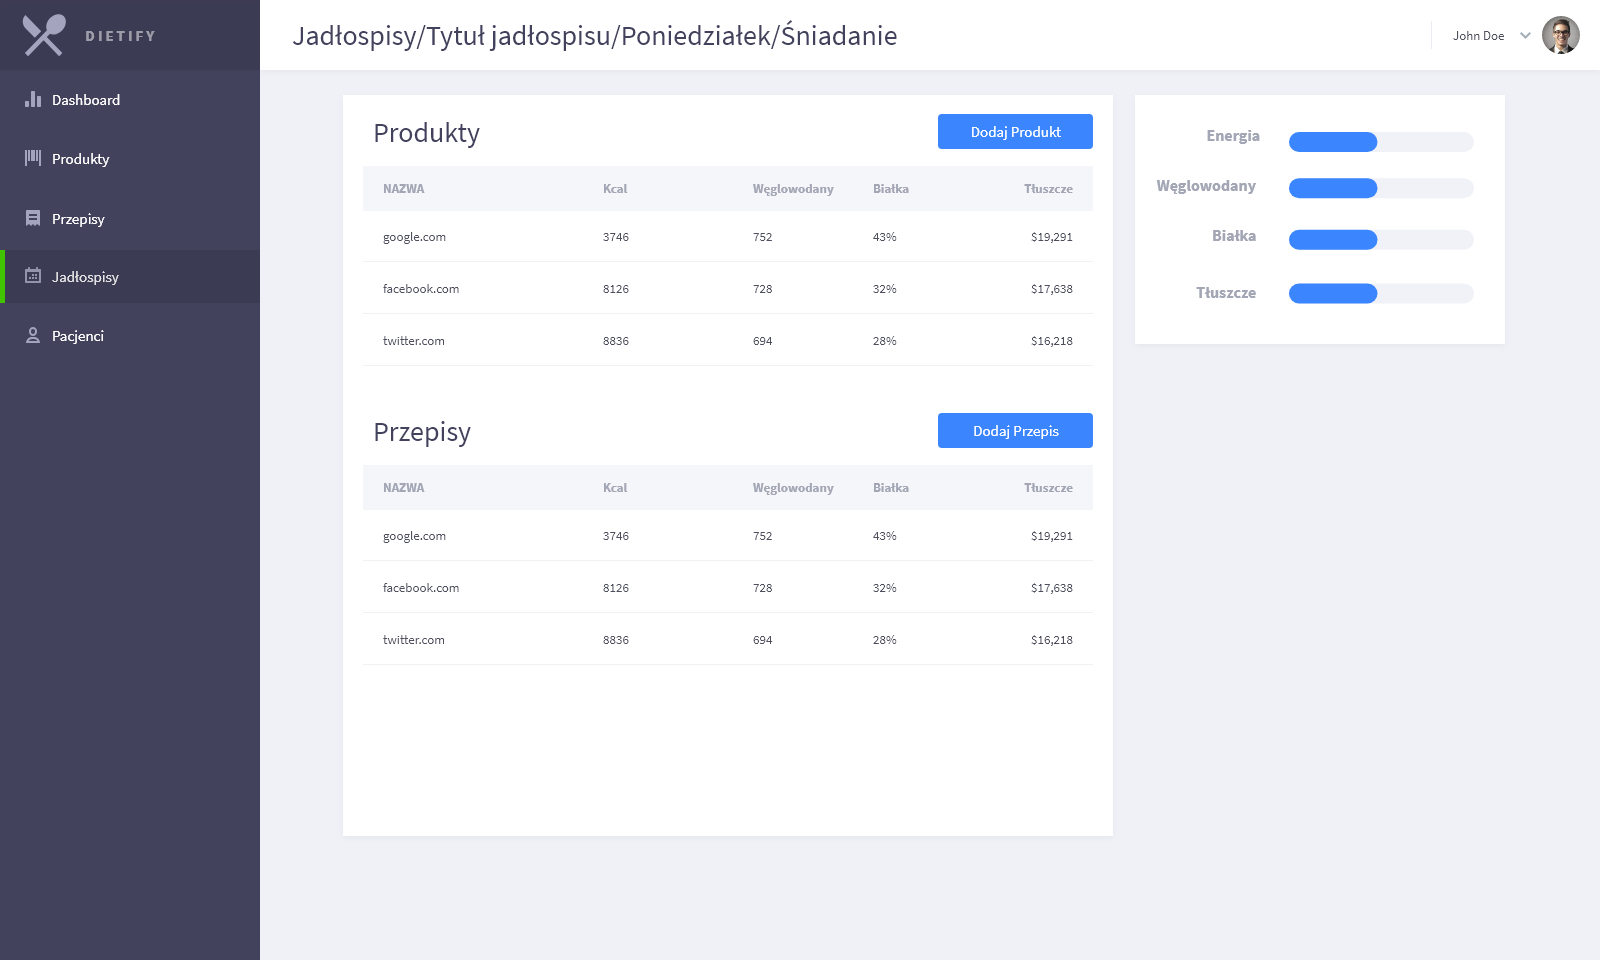
\includegraphics[width=0.9\textwidth]{img/mockups/mockup10.png}
        \caption{Mockup10 (opr.wł).}\label{rysunek:mockup10}
    \end{figure}
\end{minipage}

\begin{minipage}{\textwidth}
    \begin{figure}[H]
        \centering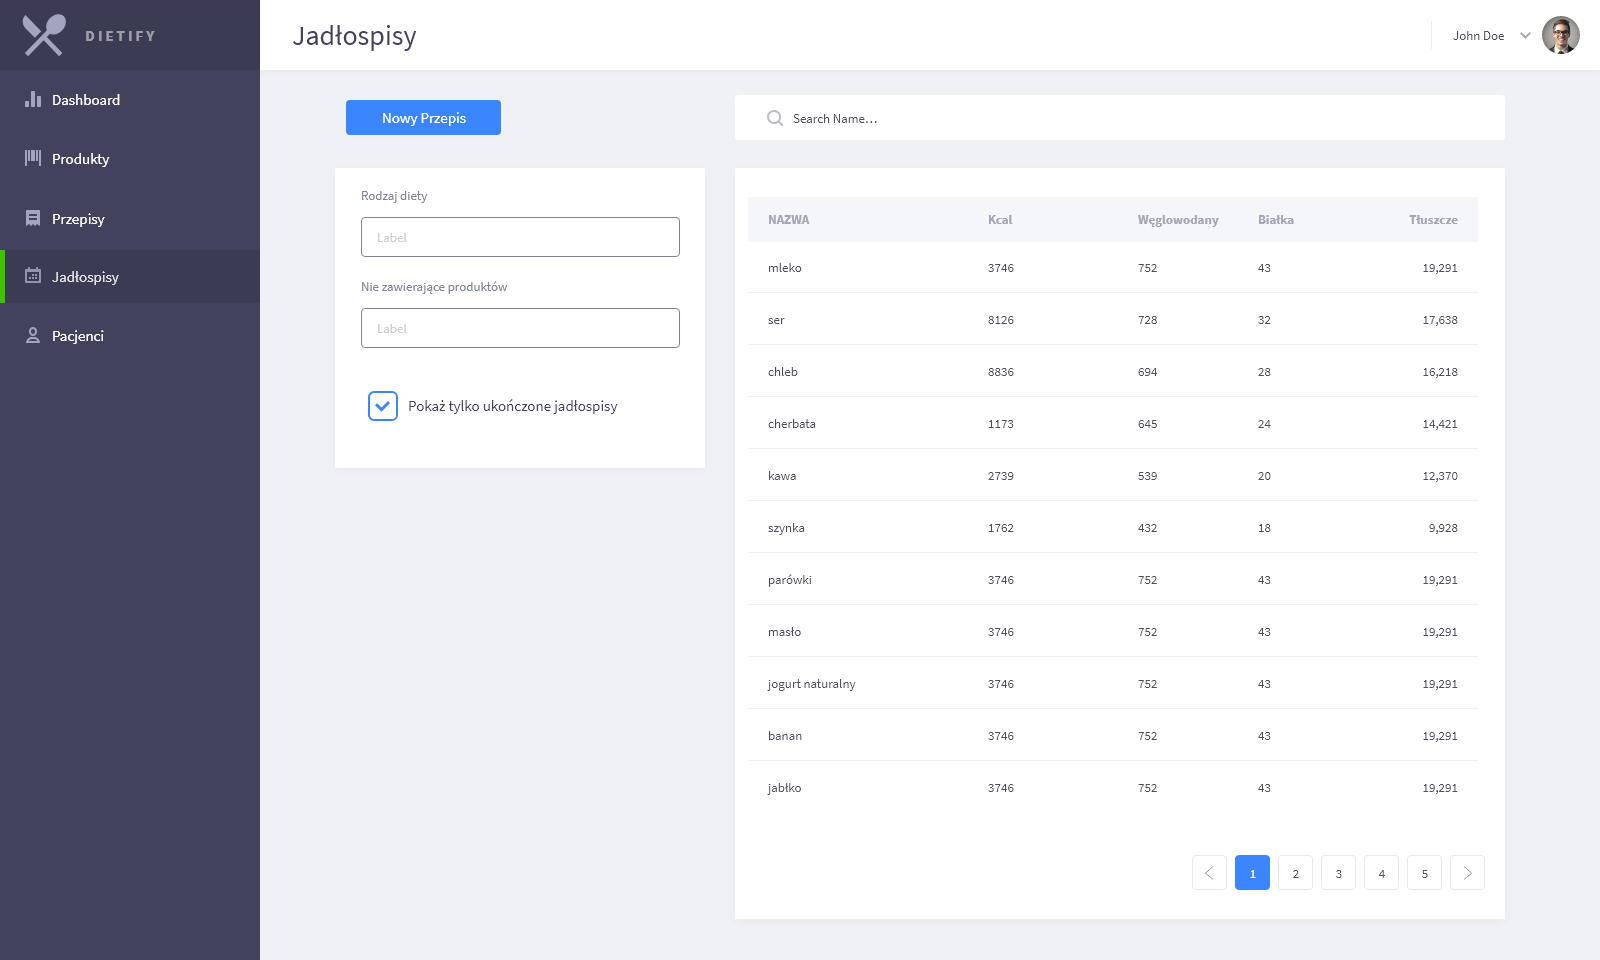
\includegraphics[width=0.9\textwidth]{img/mockups/mockup11.png}
        \caption{Mockup11 (opr.wł).}\label{rysunek:mockup11}
    \end{figure}
\end{minipage}

\begin{minipage}{\textwidth}
    \begin{figure}[H]
        \centering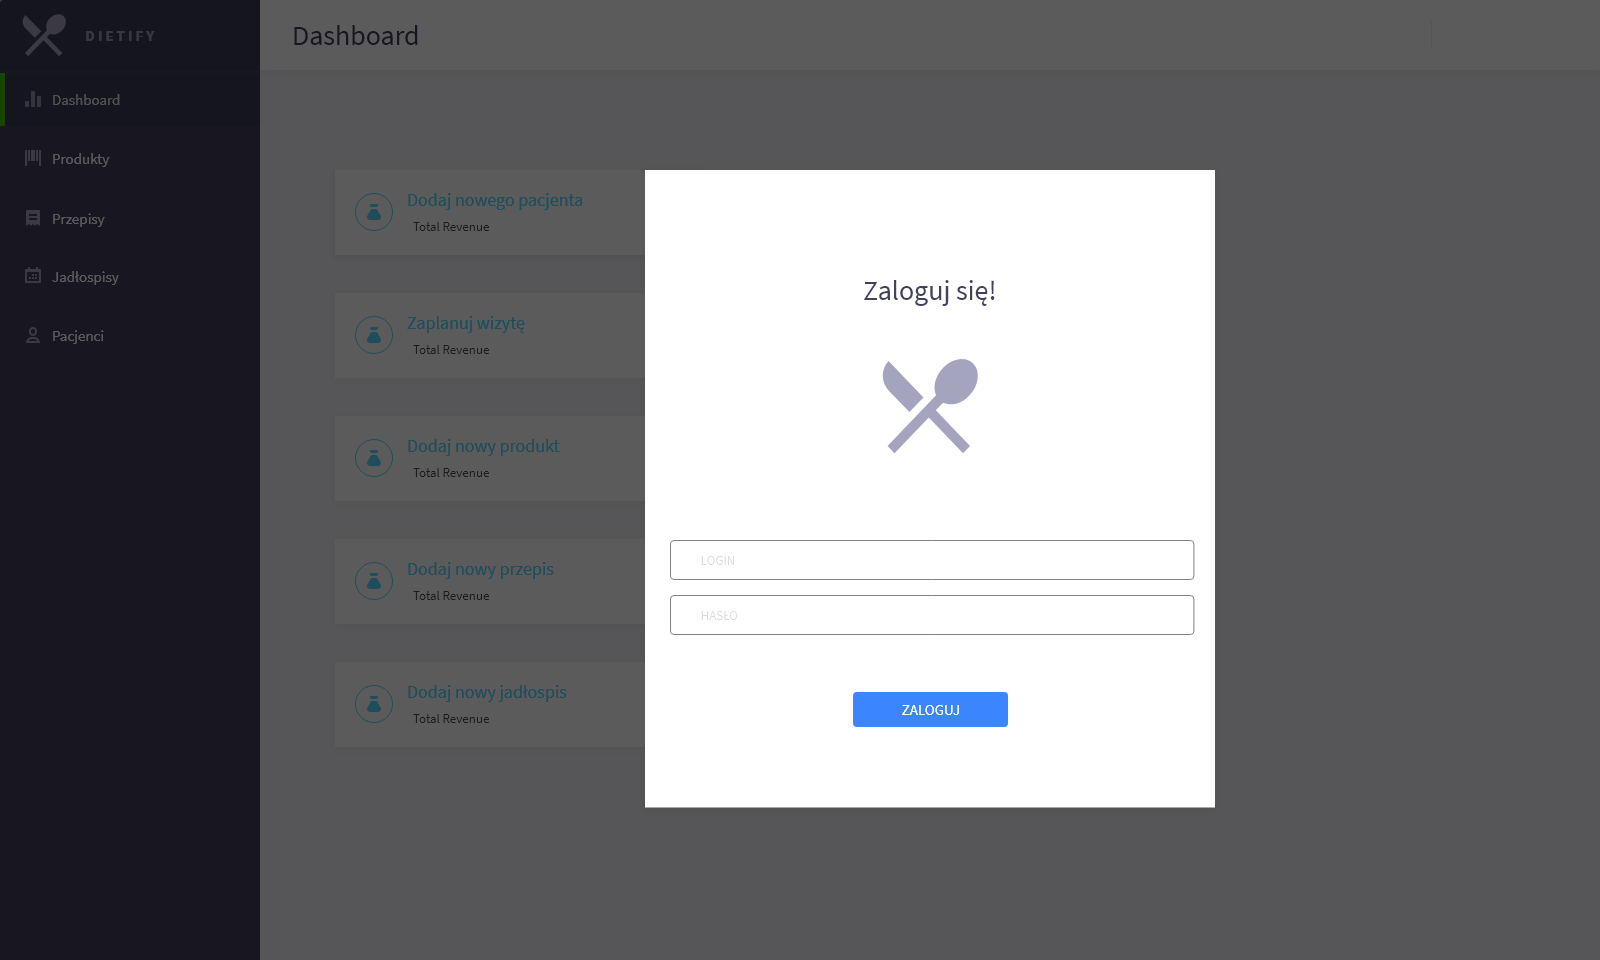
\includegraphics[width=0.9\textwidth]{img/mockups/mockup12.png}
        \caption{Mockup12 (opr.wł).}\label{rysunek:mockup12}
    \end{figure}
\end{minipage}

\begin{minipage}{\textwidth}
    \begin{figure}[H]
        \centering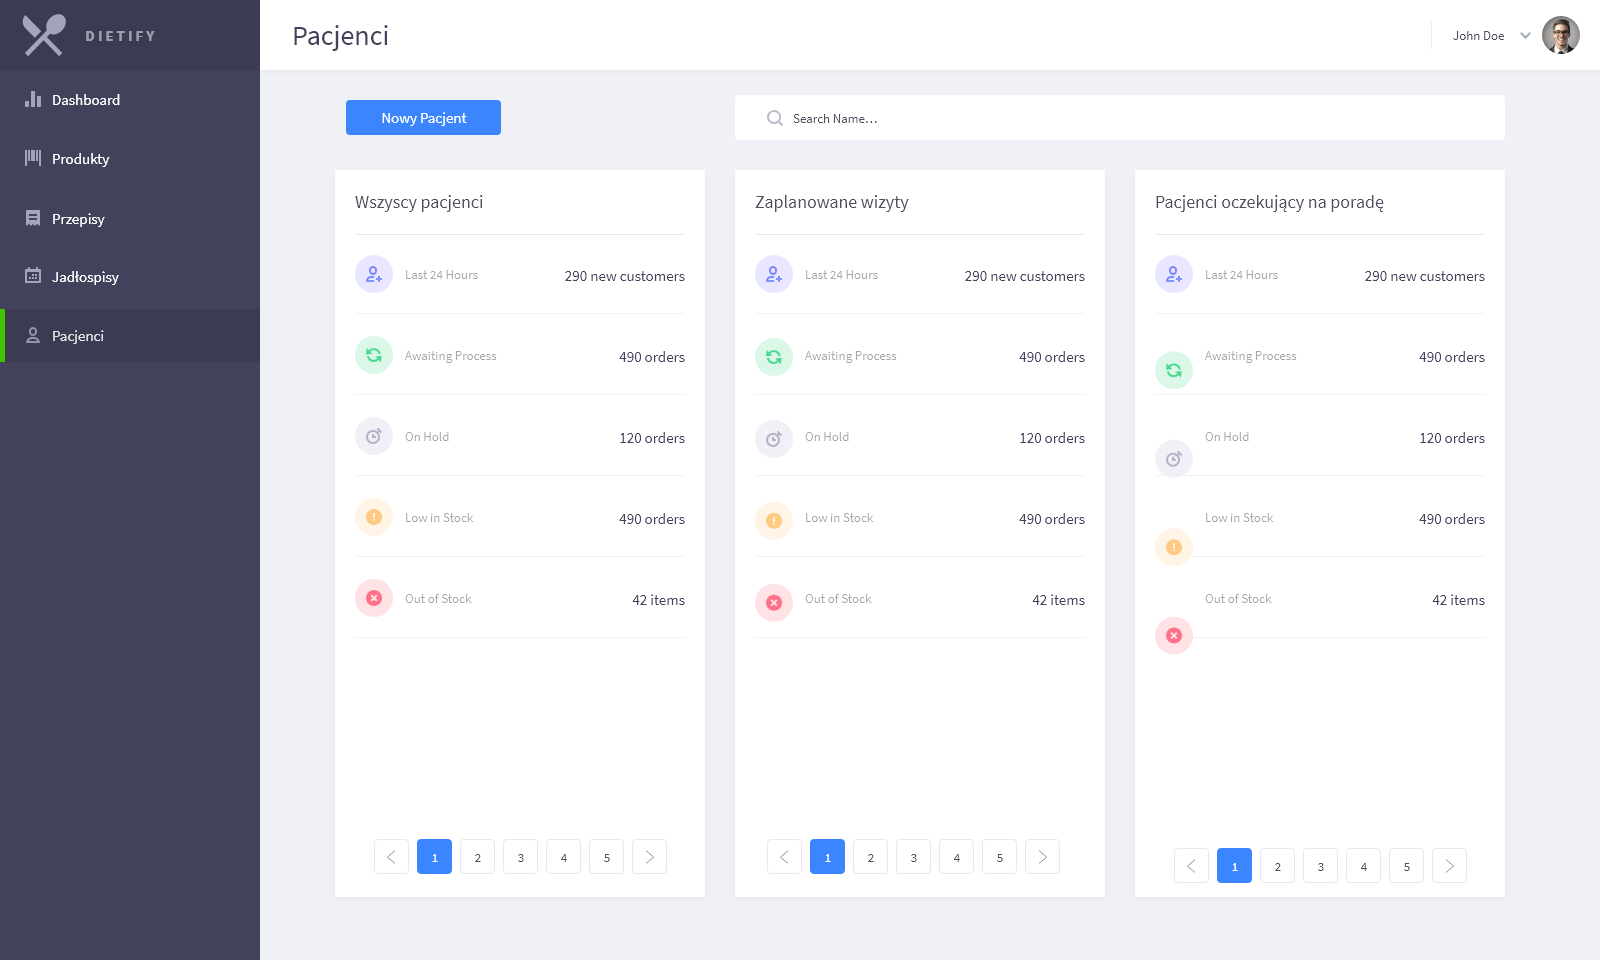
\includegraphics[width=0.9\textwidth]{img/mockups/mockup13.png}
        \caption{Mockup13 (opr.wł).}\label{rysunek:mockup13}
    \end{figure}
\end{minipage}

\begin{minipage}{\textwidth}
    \begin{figure}[H]
        \centering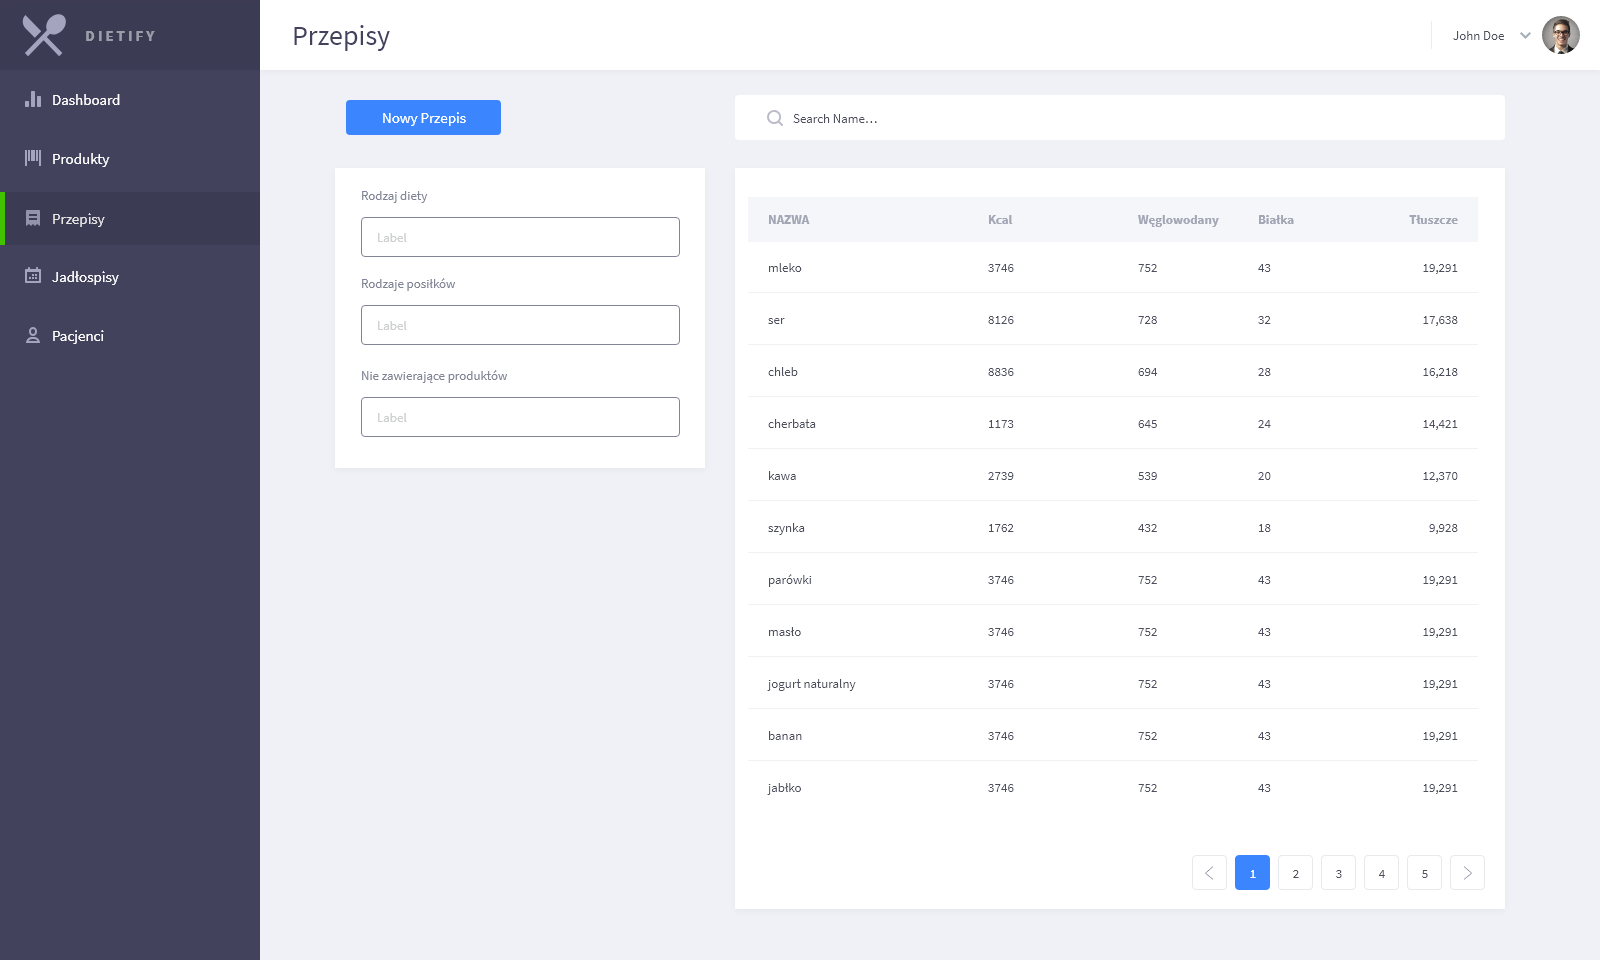
\includegraphics[width=0.9\textwidth]{img/mockups/mockup14.png}
        \caption{Mockup14 (opr.wł).}\label{rysunek:mockup14}
    \end{figure}
\end{minipage}

\begin{minipage}{\textwidth}
    \begin{figure}[H]
        \centering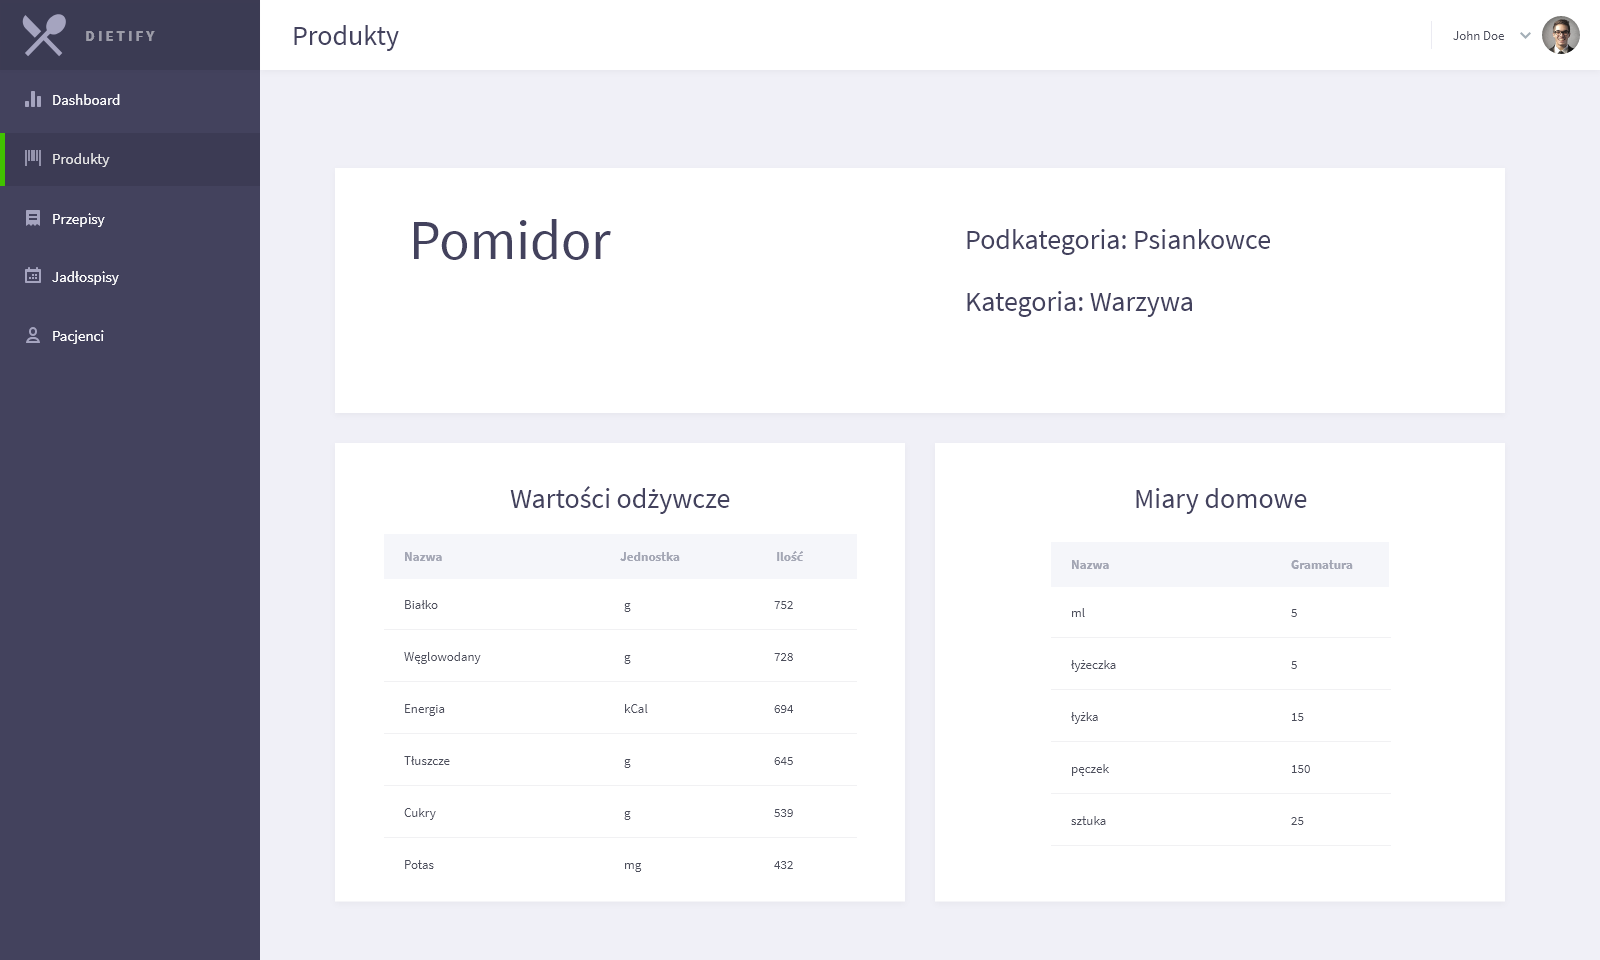
\includegraphics[width=0.9\textwidth]{img/mockups/mockup15.png}
        \caption{Mockup15 (opr.wł).}\label{rysunek:mockup15}
    \end{figure}
\end{minipage}

\begin{minipage}{\textwidth}
    \begin{figure}[H]
        \centering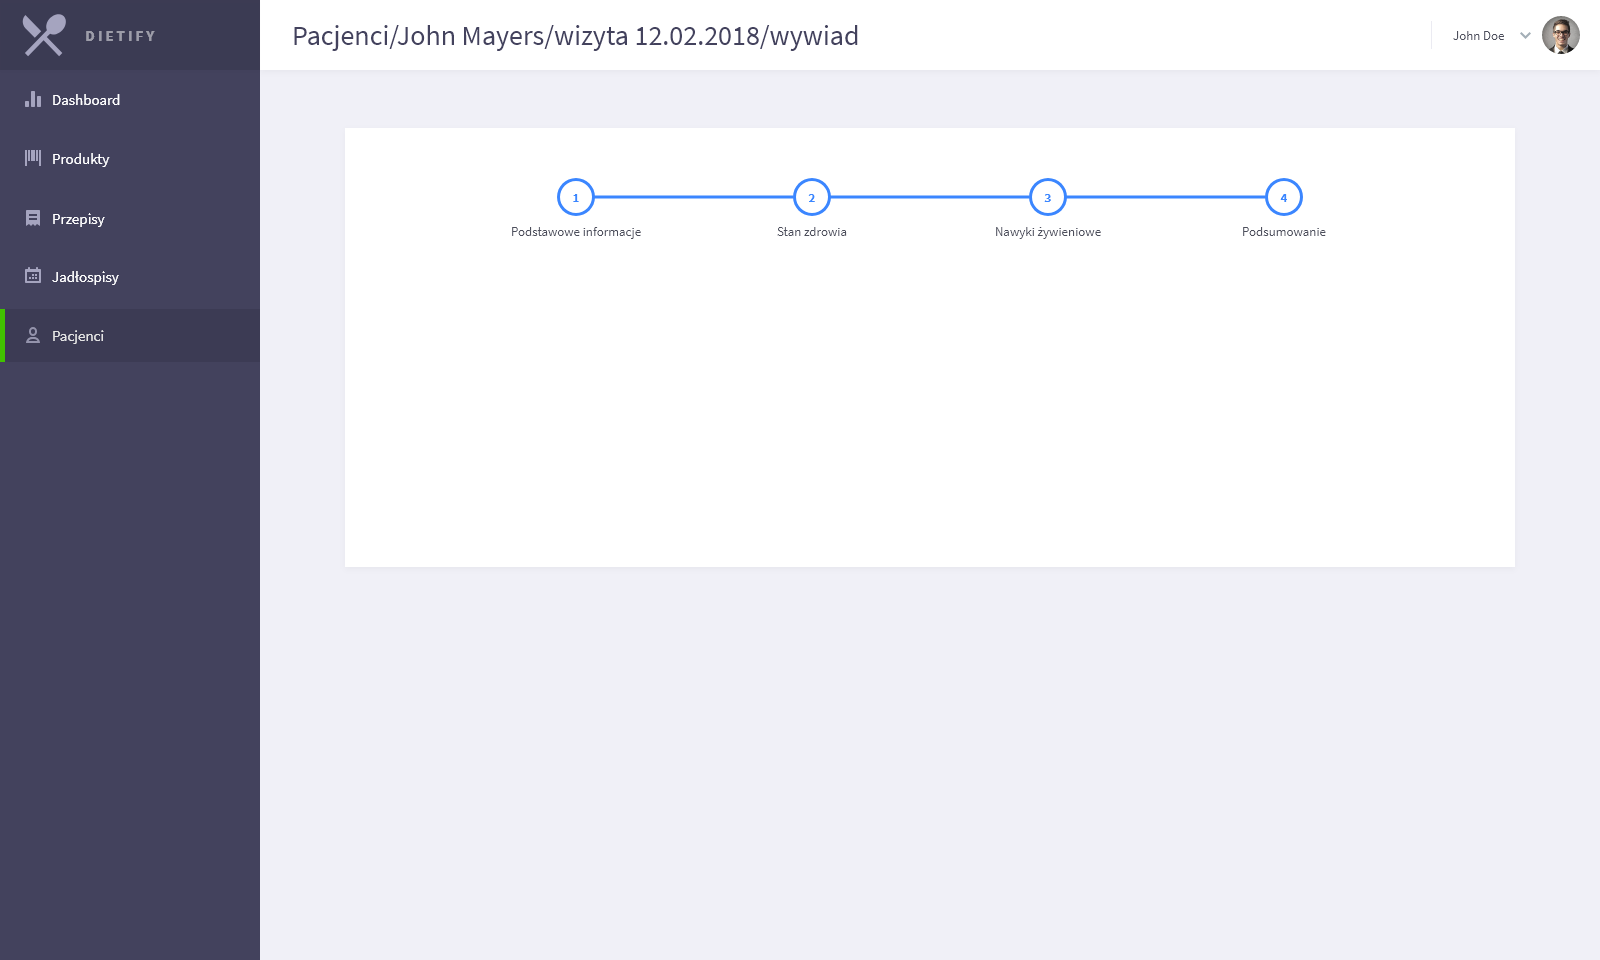
\includegraphics[width=0.9\textwidth]{img/mockups/mockup16.png}
        \caption{Mockup16 (opr.wł).}\label{rysunek:mockup16}
    \end{figure}
\end{minipage}

\section{Baza danych}

\subsection{Kategorie}
\todo{uzupełnić kategorie}

\begin{enumerate}[label={\textbf{KAT/\protect\threedigits{\theenumi}}}, wide, labelwidth=!, labelindent=0pt]
    \setlength\itemsep{1em}
    \item \label{kat:user} User

    Opis: \lipsum[1]
    \par
    Atrybuty:
    \begin{itemize}
        \item id
        \item login
        \item passwordHash
        \item firstName
        \item lastName
        \item email
        \item image
        \item activated
        \item langKey
        \item activationKey
        \item createdBy
        \item createdDate
        \item resetDate
        \item lastModifiedBy
        \item lastModifiedDate
    \end{itemize}

    \item \label{kat:UserExtraInfo} UserExtraInfo

    Opis: \lipsum[1]
    \par
    Atrybuty:
    \begin{itemize}
        \item id
        \item gender
        \item dateOfBirth
        \item phoneNumber
        \item streetAddress
        \item postalCode
        \item city
        \item country
        \item personalDescription
    \end{itemize}

    \item \label{kat:SiteContent} SiteContent

    Opis: \lipsum[1]
    \par
    Atrybuty:
    \begin{itemize}
        \item id
        \item ordinalNumber
        \item siteContentType
        \item title
        \item description
    \end{itemize}

    \item \label{kat:SiteContentTranslation} SiteContentTranslation

    Opis: \lipsum[1]
    \par
    Atrybuty:
    \begin{itemize}
        \item id
        \item title
        \item description
        \item language
    \end{itemize}

    \item \label{kat:ContactInfo} ContactInfo

    Opis: \lipsum[1]
    \par
    Atrybuty:
    \begin{itemize}
        \item id
        \item contactInfoType
        \item description
    \end{itemize}

    \item \label{kat:Pricing} Pricing

    Opis: \lipsum[1]
    \par
    Atrybuty:
    \begin{itemize}
        \item id
        \item ordinalNumber
        \item title
        \item description
        \item price
        \item currency
    \end{itemize}

    \item \label{kat:PricingTranslation} PricingTranslation

    Opis: \lipsum[1]
    \par
    Atrybuty:
    \begin{itemize}
        \item id
        \item title
        \item description
        \item language
    \end{itemize}

    \item \label{kat:Product} Product

    Opis: \lipsum[1]
    \par
    Atrybuty:
    \begin{itemize}
        \item id
        \item source
        \item isPublic
        \item language
    \end{itemize}

    \item \label{kat:ProductVersion} ProductVersion

    Opis: \lipsum[1]
    \par
    Atrybuty:
    \begin{itemize}
        \item id
        \item editTimestamp
        \item description
    \end{itemize}

    \item \label{kat:ProductBasicNutritionData} ProductBasicNutritionData

    Opis: \lipsum[1]
    \par
    Atrybuty:
    \begin{itemize}
        \item id
        \item energy
        \item protein
        \item fat
        \item carbohydrates
    \end{itemize}

    \item \label{kat:NutritionData} NutritionData

    Opis: \lipsum[1]
    \par
    Atrybuty:
    \begin{itemize}
        \item id
        \item nutritionValue
    \end{itemize}

    \item \label{kat:NutritionDefinition} NutritionDefinition

    Opis: \lipsum[1]
    \par
    Atrybuty:
    \begin{itemize}
        \item id
        \item tag
        \item description
        \item units
        \item decimalPlaces
    \end{itemize}

    \item \label{kat:NutritionDefinitionTranslation} NutritionDefinitionTranslation

    Opis: \lipsum[1]
    \par
    Atrybuty:
    \begin{itemize}
        \item id
        \item translation
        \item language
    \end{itemize}

    \item \label{kat:HouseholdMeasure} HouseholdMeasure

    Opis: \lipsum[1]
    \par
    Atrybuty:
    \begin{itemize}
        \item id
        \item description
        \item gramsWeight
        \item isVisible
    \end{itemize}

    \item \label{kat:ProductSubcategory} ProductSubcategory

    Opis: \lipsum[1]
    \par
    Atrybuty:
    \begin{itemize}
        \item id
        \item description
    \end{itemize}

    \item \label{kat:ProductCategory} ProductCategory

    Opis: \lipsum[1]
    \par
    Atrybuty:
    \begin{itemize}
        \item id
        \item description
    \end{itemize}

    \item \label{kat:ProductCategoryTranslation} ProductCategoryTranslation

    Opis: \lipsum[1]
    \par
    Atrybuty:
    \begin{itemize}
        \item id
        \item translation
        \item language
    \end{itemize}

    \item \label{kat:DietType} DietType

    Opis: \lipsum[1]
    \par
    Atrybuty:
    \begin{itemize}
        \item id
        \item name
    \end{itemize}

    \item \label{kat:DietTypeTranslation} DietTypeTranslation

    Opis: \lipsum[1]
    \par
    Atrybuty:
    \begin{itemize}
        \item id
        \item translation
        \item language
    \end{itemize}

    \item \label{kat:Recipe} Recipe

    Opis: \lipsum[1]
    \par
    Atrybuty:
    \begin{itemize}
        \item id
        \item isPublic
        \item language
    \end{itemize}

    \item \label{kat:RecipeVersion} RecipeVersion

    Opis: \lipsum[1]
    \par
    Atrybuty:
    \begin{itemize}
        \item id
        \item editTimestamp
        \item name
        \item preparationTimeMinutes
        \item numberOfPortions
        \item image
        \item totalGramsWeight
    \end{itemize}

    \item \label{kat:RecipeBasicNutritionData} RecipeBasicNutritionData

    Opis: \lipsum[1]
    \par
    Atrybuty:
    \begin{itemize}
        \item id
        \item energy
        \item protein
        \item fat
        \item carbohydrates
    \end{itemize}

    \item \label{kat:RecipeSection} RecipeSection

    Opis: \lipsum[1]
    \par
    Atrybuty:
    \begin{itemize}
        \item id
        \item sectionName
    \end{itemize}

    \item \label{kat:ProductPortion} ProductPortion

    Opis: \lipsum[1]
    \par
    Atrybuty:
    \begin{itemize}
        \item id
        \item amount
    \end{itemize}

    \item \label{kat:PreparationStep} PreparationStep

    Opis: \lipsum[1]
    \par
    Atrybuty:
    \begin{itemize}
        \item id
        \item ordinalNumber
        \item stepDescription
    \end{itemize}

    \item \label{kat:KitchenAppliance} KitchenAppliance

    Opis: \lipsum[1]
    \par
    Atrybuty:
    \begin{itemize}
        \item id
        \item name
    \end{itemize}

    \item \label{kat:KitchenApplianceTranslation} KitchenApplianceTranslation

    Opis: \lipsum[1]
    \par
    Atrybuty:
    \begin{itemize}
        \item id
        \item translation
        \item language
    \end{itemize}

    \item \label{kat:DishType} DishType

    Opis: \lipsum[1]
    \par
    Atrybuty:
    \begin{itemize}
        \item id
        \item description
    \end{itemize}

    \item \label{kat:DishTypeTranslation} DishTypeTranslation

    Opis: \lipsum[1]
    \par
    Atrybuty:
    \begin{itemize}
        \item id
        \item translation
        \item language
    \end{itemize}

    \item \label{kat:MealType} MealType

    Opis: \lipsum[1]
    \par
    Atrybuty:
    \begin{itemize}
        \item id
        \item name
    \end{itemize}

    \item \label{kat:MealTypeTranslation} MealTypeTranslation

    Opis: \lipsum[1]
    \par
    Atrybuty:
    \begin{itemize}
        \item id
        \item translation
        \item language
    \end{itemize}


    \item \label{kat:MealPlan} MealPlan

    Opis: \lipsum[1]
    \par
    Atrybuty:
    \begin{itemize}
        \item id
        \item creationTimestamp
        \item editTimestamp
        \item name
        \item isVisible
        \item language
        \item numberOfDays
        \item numberOfMealsPerDay
        \item totalDailyEnergy
        \item percentOfProtein
        \item percentOfFat
        \item percentOfCarbohydrates
    \end{itemize}

    \item \label{kat:MealPlanDay} MealPlanDay

    Opis: \lipsum[1]
    \par
    Atrybuty:
    \begin{itemize}
        \item id
        \item ordinalNumber
    \end{itemize}

    \item \label{kat:Meal} Meal

    Opis: \lipsum[1]
    \par
    Atrybuty:
    \begin{itemize}
        \item id
        \item ordinalNumber
    \end{itemize}

    \item \label{kat:MealRecipe} MealRecipe

    Opis: \lipsum[1]
    \par
    Atrybuty:
    \begin{itemize}
        \item id
        \item amount
    \end{itemize}

    \item \label{kat:MealProduct} MealProduct

    Opis: \lipsum[1]
    \par
    Atrybuty:
    \begin{itemize}
        \item id
        \item amount
    \end{itemize}

    \item \label{kat:MealDefinition} MealDefinition

    Opis: \lipsum[1]
    \par
    Atrybuty:
    \begin{itemize}
        \item id
        \item ordinalNumber
        \item timeOfMeal
        \item percentOfEnergy
    \end{itemize}

    \item \label{kat:Appointment} Appointment

    Opis: \lipsum[1]
    \par
    Atrybuty:
    \begin{itemize}
        \item id
        \item appointmentDate
        \item appointmentState
        \item generalAdvice
    \end{itemize}

    \item \label{kat:PatientCard} PatientCard

    Opis: \lipsum[1]
    \par
    Atrybuty:
    \begin{itemize}
        \item id
        \item creationDate
    \end{itemize}

    \item \label{kat:AppointmentEvaluation} AppointmentEvaluation

    Opis: \lipsum[1]
    \par
    Atrybuty:
    \begin{itemize}
        \item id
        \item overallSatisfaction
        \item dietitianServiceSatisfaction
        \item mealPlanOverallSatisfaction
        \item mealCostSatisfaction
        \item mealPreparationTimeSatisfaction
        \item mealComplexityLevelSatisfaction
        \item mealTastefulnessSatisfaction
        \item dietaryResultSatisfaction
        \item comment
    \end{itemize}

    \item \label{kat:BodyMeasurement} BodyMeasurement

    Opis: \lipsum[1]
    \par
    Atrybuty:
    \begin{itemize}
        \item id
        \item completionDate
        \item height
        \item weight
        \item waist
        \item percentOfFatTissue
        \item percentOfWater
        \item muscleMass
        \item physicalMark
        \item calciumInBones
        \item basicMetabolism
        \item metabolicAge
        \item visceralDatLevel
    \end{itemize}

    \item \label{kat:NutritionalInterview} NutritionalInterview

    Opis: \lipsum[1]
    \par
    Atrybuty:
    \begin{itemize}
        \item id
        \item completionDate
        \item targetWeight
        \item advicePurpose
        \item physicalActivity
        \item diseases
        \item medicines
        \item jobType
        \item likedProducts
        \item dislikedProducts
        \item foodAllergies
        \item foodIntolerances
    \end{itemize}

    \item \label{kat:OwnedKitchenAppliance} OwnedKitchenAppliance

    Opis: \lipsum[1]
    \par
    Atrybuty:
    \begin{itemize}
        \item id
    \end{itemize}

    \item \label{kat:CustomNutritionalInterviewQuestion} CustomNutritionalInterviewQuestion

    Opis: \lipsum[1]
    \par
    Atrybuty:
    \begin{itemize}
        \item id
        \item ordinalNumber
        \item question
        \item answer
    \end{itemize}

    \item \label{kat:CustomNutritionalInterviewQuestionTemplate} CustomNutritionalInterviewQuestionTemplate

    Opis: \lipsum[1]
    \par
    Atrybuty:
    \begin{itemize}
        \item id
        \item question
        \item language
    \end{itemize}

    \item \label{kat:AssignedMealPlan} AssignedMealPlan

    Opis: \lipsum[1]
    \par
    Atrybuty:
    \begin{itemize}
        \item id
        \item assigmentTime
    \end{itemize}


\end{enumerate}

\subsection {Reguły funkcjonowania}
\todo{uzupełnić reguły funkcjonowania, i.e. związki pomiędzy encjami}

\begin{itemize}[label={}]
    \setlength\itemsep{1em}
    \item Reguły dla \ref{kat:user} User
    \begin{enumerate}[label={\textbf{REG/\protect\threedigits{\arabic{enumi}}}}, wide, labelwidth=!]
        \item test1
        \item test2
    \end{enumerate}
    \item Reguły dla \ref{kat:UserExtraInfo} UserExtraInfo
    \begin{enumerate}[label={\textbf{REG/\protect\threedigits{\arabic{enumi}}}}, wide, labelwidth=!, resume]
        \item test1
        \item test2
    \end{enumerate}
    \item Reguły dla \ref{kat:SiteContent} SiteContent
    \begin{enumerate}[label={\textbf{REG/\protect\threedigits{\arabic{enumi}}}}, wide, labelwidth=!, resume]
        \item test1
        \item test2
    \end{enumerate}
    \item Reguły dla \ref{kat:SiteContentTranslation} SiteContentTranslation
    \begin{enumerate}[label={\textbf{REG/\protect\threedigits{\arabic{enumi}}}}, wide, labelwidth=!, resume]
        \item test1
        \item test2
    \end{enumerate}
    \item Reguły dla \ref{kat:ContactInfo} ContactInfo
    \begin{enumerate}[label={\textbf{REG/\protect\threedigits{\arabic{enumi}}}}, wide, labelwidth=!, resume]
        \item test1
        \item test2
    \end{enumerate}
    \item Reguły dla \ref{kat:Pricing} Pricing
    \begin{enumerate}[label={\textbf{REG/\protect\threedigits{\arabic{enumi}}}}, wide, labelwidth=!, resume]
        \item test1
        \item test2
    \end{enumerate}
    \item Reguły dla \ref{kat:PricingTranslation} PricingTranslation
    \begin{enumerate}[label={\textbf{REG/\protect\threedigits{\arabic{enumi}}}}, wide, labelwidth=!, resume]
        \item test1
        \item test2
    \end{enumerate}
    \item Reguły dla \ref{kat:Product} Product
    \begin{enumerate}[label={\textbf{REG/\protect\threedigits{\arabic{enumi}}}}, wide, labelwidth=!, resume]
        \item test1
        \item test2
    \end{enumerate}
    \item Reguły dla \ref{kat:ProductVersion} ProductVersion
    \begin{enumerate}[label={\textbf{REG/\protect\threedigits{\arabic{enumi}}}}, wide, labelwidth=!, resume]
        \item test1
        \item test2
    \end{enumerate}
    \item Reguły dla \ref{kat:ProductBasicNutritionData} ProductBasicNutritionData
    \begin{enumerate}[label={\textbf{REG/\protect\threedigits{\arabic{enumi}}}}, wide, labelwidth=!, resume]
        \item test1
        \item test2
    \end{enumerate}
    \item Reguły dla \ref{kat:NutritionData} NutritionData
    \begin{enumerate}[label={\textbf{REG/\protect\threedigits{\arabic{enumi}}}}, wide, labelwidth=!, resume]
        \item test1
        \item test2
    \end{enumerate}
    \item Reguły dla \ref{kat:NutritionDefinition} NutritionDefinition
    \begin{enumerate}[label={\textbf{REG/\protect\threedigits{\arabic{enumi}}}}, wide, labelwidth=!, resume]
        \item test1
        \item test2
    \end{enumerate}
    \item Reguły dla \ref{kat:NutritionDefinitionTranslation} NutritionDefinitionTranslation
    \begin{enumerate}[label={\textbf{REG/\protect\threedigits{\arabic{enumi}}}}, wide, labelwidth=!, resume]
        \item test1
        \item test2
    \end{enumerate}
    \item Reguły dla \ref{kat:HouseholdMeasure} HouseholdMeasure
    \begin{enumerate}[label={\textbf{REG/\protect\threedigits{\arabic{enumi}}}}, wide, labelwidth=!, resume]
        \item test1
        \item test2
    \end{enumerate}
    \item Reguły dla \ref{kat:ProductSubcategory} ProductSubcategory
    \begin{enumerate}[label={\textbf{REG/\protect\threedigits{\arabic{enumi}}}}, wide, labelwidth=!, resume]
        \item test1
        \item test2
    \end{enumerate}
    \item Reguły dla \ref{kat:ProductCategory} ProductCategory
    \begin{enumerate}[label={\textbf{REG/\protect\threedigits{\arabic{enumi}}}}, wide, labelwidth=!, resume]
        \item test1
        \item test2
    \end{enumerate}
    \item Reguły dla \ref{kat:ProductCategoryTranslation} ProductCategoryTranslation
    \begin{enumerate}[label={\textbf{REG/\protect\threedigits{\arabic{enumi}}}}, wide, labelwidth=!, resume]
        \item test1
        \item test2
    \end{enumerate}
    \item Reguły dla \ref{kat:DietType} DietType
    \begin{enumerate}[label={\textbf{REG/\protect\threedigits{\arabic{enumi}}}}, wide, labelwidth=!, resume]
        \item test1
        \item test2
    \end{enumerate}
    \item Reguły dla \ref{kat:DietTypeTranslation} DietTypeTranslation
    \begin{enumerate}[label={\textbf{REG/\protect\threedigits{\arabic{enumi}}}}, wide, labelwidth=!, resume]
        \item test1
        \item test2
    \end{enumerate}
    \item Reguły dla \ref{kat:Recipe} Recipe
    \begin{enumerate}[label={\textbf{REG/\protect\threedigits{\arabic{enumi}}}}, wide, labelwidth=!, resume]
        \item test1
        \item test2
    \end{enumerate}
    \item Reguły dla \ref{kat:RecipeVersion} RecipeVersion
    \begin{enumerate}[label={\textbf{REG/\protect\threedigits{\arabic{enumi}}}}, wide, labelwidth=!, resume]
        \item test1
        \item test2
    \end{enumerate}
    \item Reguły dla \ref{kat:RecipeBasicNutritionData} RecipeBasicNutritionData
    \begin{enumerate}[label={\textbf{REG/\protect\threedigits{\arabic{enumi}}}}, wide, labelwidth=!, resume]
        \item test1
        \item test2
    \end{enumerate}
    \item Reguły dla \ref{kat:RecipeSection} RecipeSection
    \begin{enumerate}[label={\textbf{REG/\protect\threedigits{\arabic{enumi}}}}, wide, labelwidth=!, resume]
        \item test1
        \item test2
    \end{enumerate}
    \item Reguły dla \ref{kat:ProductPortion} ProductPortion
    \begin{enumerate}[label={\textbf{REG/\protect\threedigits{\arabic{enumi}}}}, wide, labelwidth=!, resume]
        \item test1
        \item test2
    \end{enumerate}
    \item Reguły dla \ref{kat:PreparationStep} PreparationStep
    \begin{enumerate}[label={\textbf{REG/\protect\threedigits{\arabic{enumi}}}}, wide, labelwidth=!, resume]
        \item test1
        \item test2
    \end{enumerate}
    \item Reguły dla \ref{kat:KitchenAppliance} KitchenAppliance
    \begin{enumerate}[label={\textbf{REG/\protect\threedigits{\arabic{enumi}}}}, wide, labelwidth=!, resume]
        \item test1
        \item test2
    \end{enumerate}
    \item Reguły dla \ref{kat:KitchenApplianceTranslation} KitchenApplianceTranslation
    \begin{enumerate}[label={\textbf{REG/\protect\threedigits{\arabic{enumi}}}}, wide, labelwidth=!, resume]
        \item test1
        \item test2
    \end{enumerate}
    \item Reguły dla \ref{kat:DishType} DishType
    \begin{enumerate}[label={\textbf{REG/\protect\threedigits{\arabic{enumi}}}}, wide, labelwidth=!, resume]
        \item test1
        \item test2
    \end{enumerate}
    \item Reguły dla \ref{kat:DishTypeTranslation} DishTypeTranslation
    \begin{enumerate}[label={\textbf{REG/\protect\threedigits{\arabic{enumi}}}}, wide, labelwidth=!, resume]
        \item test1
        \item test2
    \end{enumerate}
    \item Reguły dla \ref{kat:MealType} MealType
    \begin{enumerate}[label={\textbf{REG/\protect\threedigits{\arabic{enumi}}}}, wide, labelwidth=!, resume]
        \item test1
        \item test2
    \end{enumerate}
    \item Reguły dla \ref{kat:MealTypeTranslation} MealTypeTranslation
    \begin{enumerate}[label={\textbf{REG/\protect\threedigits{\arabic{enumi}}}}, wide, labelwidth=!, resume]
        \item test1
        \item test2
    \end{enumerate}
    \item Reguły dla \ref{kat:MealPlan} MealPlan
    \begin{enumerate}[label={\textbf{REG/\protect\threedigits{\arabic{enumi}}}}, wide, labelwidth=!, resume]
        \item test1
        \item test2
    \end{enumerate}
    \item Reguły dla \ref{kat:MealPlanDay} MealPlanDay
    \begin{enumerate}[label={\textbf{REG/\protect\threedigits{\arabic{enumi}}}}, wide, labelwidth=!, resume]
        \item test1
        \item test2
    \end{enumerate}
    \item Reguły dla \ref{kat:Meal} Meal
    \begin{enumerate}[label={\textbf{REG/\protect\threedigits{\arabic{enumi}}}}, wide, labelwidth=!, resume]
        \item test1
        \item test2
    \end{enumerate}
    \item Reguły dla \ref{kat:MealRecipe} MealRecipe
    \begin{enumerate}[label={\textbf{REG/\protect\threedigits{\arabic{enumi}}}}, wide, labelwidth=!, resume]
        \item test1
        \item test2
    \end{enumerate}
    \item Reguły dla \ref{kat:MealProduct} MealProduct
    \begin{enumerate}[label={\textbf{REG/\protect\threedigits{\arabic{enumi}}}}, wide, labelwidth=!, resume]
        \item test1
        \item test2
    \end{enumerate}
    \item Reguły dla \ref{kat:MealDefinition} MealDefinition
    \begin{enumerate}[label={\textbf{REG/\protect\threedigits{\arabic{enumi}}}}, wide, labelwidth=!, resume]
        \item test1
        \item test2
    \end{enumerate}
    \item Reguły dla \ref{kat:Appointment} Appointment
    \begin{enumerate}[label={\textbf{REG/\protect\threedigits{\arabic{enumi}}}}, wide, labelwidth=!, resume]
        \item test1
        \item test2
    \end{enumerate}
    \item Reguły dla \ref{kat:PatientCard} PatientCard
    \begin{enumerate}[label={\textbf{REG/\protect\threedigits{\arabic{enumi}}}}, wide, labelwidth=!, resume]
        \item test1
        \item test2
    \end{enumerate}
    \item Reguły dla \ref{kat:AppointmentEvaluation} AppointmentEvaluation
    \begin{enumerate}[label={\textbf{REG/\protect\threedigits{\arabic{enumi}}}}, wide, labelwidth=!, resume]
        \item test1
        \item test2
    \end{enumerate}
    \item Reguły dla \ref{kat:BodyMeasurement} BodyMeasurement
    \begin{enumerate}[label={\textbf{REG/\protect\threedigits{\arabic{enumi}}}}, wide, labelwidth=!, resume]
        \item test1
        \item test2
    \end{enumerate}
    \item Reguły dla \ref{kat:NutritionalInterview} NutritionalInterview
    \begin{enumerate}[label={\textbf{REG/\protect\threedigits{\arabic{enumi}}}}, wide, labelwidth=!, resume]
        \item test1
        \item test2
    \end{enumerate}
    \item Reguły dla \ref{kat:OwnedKitchenAppliance} OwnedKitchenAppliance
    \begin{enumerate}[label={\textbf{REG/\protect\threedigits{\arabic{enumi}}}}, wide, labelwidth=!, resume]
        \item test1
        \item test2
    \end{enumerate}
    \item Reguły dla \ref{kat:CustomNutritionalInterviewQuestion} CustomNutritionalInterviewQuestion
    \begin{enumerate}[label={\textbf{REG/\protect\threedigits{\arabic{enumi}}}}, wide, labelwidth=!, resume]
        \item test1
        \item test2
    \end{enumerate}
    \item Reguły dla \ref{kat:CustomNutritionalInterviewQuestionTemplate} CustomNutritionalInterviewQuestionTemplate
    \begin{enumerate}[label={\textbf{REG/\protect\threedigits{\arabic{enumi}}}}, wide, labelwidth=!, resume]
        \item test1
        \item test2
    \end{enumerate}
    \item Reguły dla \ref{kat:AssignedMealPlan} AssignedMealPlan
    \begin{enumerate}[label={\textbf{REG/\protect\threedigits{\arabic{enumi}}}}, wide, labelwidth=!, resume]
        \item test1
        \item test2
    \end{enumerate}
\end{itemize}

\subsection{Ograniczenia dziedzinowe}
\todo{uzupełnić ograniczenia dziedzionowe}

\begin{itemize}[label={}]
    \setlength\itemsep{1em}
    \item Ograniczenia dla \ref{kat:user} User
    \begin{enumerate}[label={\textbf{OGR/\protect\threedigits{\arabic{enumi}}}}, wide, labelwidth=!]
        \item test1
        \item test2
    \end{enumerate}
    \item Ograniczenia dla \ref{kat:UserExtraInfo} UserExtraInfo
    \begin{enumerate}[label={\textbf{OGR/\protect\threedigits{\arabic{enumi}}}}, wide, labelwidth=!, resume]
        \item test1
        \item test2
    \end{enumerate}
    \item Ograniczenia dla \ref{kat:SiteContent} SiteContent
    \begin{enumerate}[label={\textbf{OGR/\protect\threedigits{\arabic{enumi}}}}, wide, labelwidth=!, resume]
        \item test1
        \item test2
    \end{enumerate}
    \item Ograniczenia dla \ref{kat:SiteContentTranslation} SiteContentTranslation
    \begin{enumerate}[label={\textbf{OGR/\protect\threedigits{\arabic{enumi}}}}, wide, labelwidth=!, resume]
        \item test1
        \item test2
    \end{enumerate}
    \item Ograniczenia dla \ref{kat:ContactInfo} ContactInfo
    \begin{enumerate}[label={\textbf{OGR/\protect\threedigits{\arabic{enumi}}}}, wide, labelwidth=!, resume]
        \item test1
        \item test2
    \end{enumerate}
    \item Ograniczenia dla \ref{kat:Pricing} Pricing
    \begin{enumerate}[label={\textbf{OGR/\protect\threedigits{\arabic{enumi}}}}, wide, labelwidth=!, resume]
        \item test1
        \item test2
    \end{enumerate}
    \item Ograniczenia dla \ref{kat:PricingTranslation} PricingTranslation
    \begin{enumerate}[label={\textbf{OGR/\protect\threedigits{\arabic{enumi}}}}, wide, labelwidth=!, resume]
        \item test1
        \item test2
    \end{enumerate}
    \item Ograniczenia dla \ref{kat:Product} Product
    \begin{enumerate}[label={\textbf{OGR/\protect\threedigits{\arabic{enumi}}}}, wide, labelwidth=!, resume]
        \item test1
        \item test2
    \end{enumerate}
    \item Ograniczenia dla \ref{kat:ProductVersion} ProductVersion
    \begin{enumerate}[label={\textbf{OGR/\protect\threedigits{\arabic{enumi}}}}, wide, labelwidth=!, resume]
        \item test1
        \item test2
    \end{enumerate}
    \item Ograniczenia dla \ref{kat:ProductBasicNutritionData} ProductBasicNutritionData
    \begin{enumerate}[label={\textbf{OGR/\protect\threedigits{\arabic{enumi}}}}, wide, labelwidth=!, resume]
        \item test1
        \item test2
    \end{enumerate}
    \item Ograniczenia dla \ref{kat:NutritionData} NutritionData
    \begin{enumerate}[label={\textbf{OGR/\protect\threedigits{\arabic{enumi}}}}, wide, labelwidth=!, resume]
        \item test1
        \item test2
    \end{enumerate}
    \item Ograniczenia dla \ref{kat:NutritionDefinition} NutritionDefinition
    \begin{enumerate}[label={\textbf{OGR/\protect\threedigits{\arabic{enumi}}}}, wide, labelwidth=!, resume]
        \item test1
        \item test2
    \end{enumerate}
    \item Ograniczenia dla \ref{kat:NutritionDefinitionTranslation} NutritionDefinitionTranslation
    \begin{enumerate}[label={\textbf{OGR/\protect\threedigits{\arabic{enumi}}}}, wide, labelwidth=!, resume]
        \item test1
        \item test2
    \end{enumerate}
    \item Ograniczenia dla \ref{kat:HouseholdMeasure} HouseholdMeasure
    \begin{enumerate}[label={\textbf{OGR/\protect\threedigits{\arabic{enumi}}}}, wide, labelwidth=!, resume]
        \item test1
        \item test2
    \end{enumerate}
    \item Ograniczenia dla \ref{kat:ProductSubcategory} ProductSubcategory
    \begin{enumerate}[label={\textbf{OGR/\protect\threedigits{\arabic{enumi}}}}, wide, labelwidth=!, resume]
        \item test1
        \item test2
    \end{enumerate}
    \item Ograniczenia dla \ref{kat:ProductCategory} ProductCategory
    \begin{enumerate}[label={\textbf{OGR/\protect\threedigits{\arabic{enumi}}}}, wide, labelwidth=!, resume]
        \item test1
        \item test2
    \end{enumerate}
    \item Ograniczenia dla \ref{kat:ProductCategoryTranslation} ProductCategoryTranslation
    \begin{enumerate}[label={\textbf{OGR/\protect\threedigits{\arabic{enumi}}}}, wide, labelwidth=!, resume]
        \item test1
        \item test2
    \end{enumerate}
    \item Ograniczenia dla \ref{kat:DietType} DietType
    \begin{enumerate}[label={\textbf{OGR/\protect\threedigits{\arabic{enumi}}}}, wide, labelwidth=!, resume]
        \item test1
        \item test2
    \end{enumerate}
    \item Ograniczenia dla \ref{kat:DietTypeTranslation} DietTypeTranslation
    \begin{enumerate}[label={\textbf{OGR/\protect\threedigits{\arabic{enumi}}}}, wide, labelwidth=!, resume]
        \item test1
        \item test2
    \end{enumerate}
    \item Ograniczenia dla \ref{kat:Recipe} Recipe
    \begin{enumerate}[label={\textbf{OGR/\protect\threedigits{\arabic{enumi}}}}, wide, labelwidth=!, resume]
        \item test1
        \item test2
    \end{enumerate}
    \item Ograniczenia dla \ref{kat:RecipeVersion} RecipeVersion
    \begin{enumerate}[label={\textbf{OGR/\protect\threedigits{\arabic{enumi}}}}, wide, labelwidth=!, resume]
        \item test1
        \item test2
    \end{enumerate}
    \item Ograniczenia dla \ref{kat:RecipeBasicNutritionData} RecipeBasicNutritionData
    \begin{enumerate}[label={\textbf{OGR/\protect\threedigits{\arabic{enumi}}}}, wide, labelwidth=!, resume]
        \item test1
        \item test2
    \end{enumerate}
    \item Ograniczenia dla \ref{kat:RecipeSection} RecipeSection
    \begin{enumerate}[label={\textbf{OGR/\protect\threedigits{\arabic{enumi}}}}, wide, labelwidth=!, resume]
        \item test1
        \item test2
    \end{enumerate}
    \item Ograniczenia dla \ref{kat:ProductPortion} ProductPortion
    \begin{enumerate}[label={\textbf{OGR/\protect\threedigits{\arabic{enumi}}}}, wide, labelwidth=!, resume]
        \item test1
        \item test2
    \end{enumerate}
    \item Ograniczenia dla \ref{kat:PreparationStep} PreparationStep
    \begin{enumerate}[label={\textbf{OGR/\protect\threedigits{\arabic{enumi}}}}, wide, labelwidth=!, resume]
        \item test1
        \item test2
    \end{enumerate}
    \item Ograniczenia dla \ref{kat:KitchenAppliance} KitchenAppliance
    \begin{enumerate}[label={\textbf{OGR/\protect\threedigits{\arabic{enumi}}}}, wide, labelwidth=!, resume]
        \item test1
        \item test2
    \end{enumerate}
    \item Ograniczenia dla \ref{kat:KitchenApplianceTranslation} KitchenApplianceTranslation
    \begin{enumerate}[label={\textbf{OGR/\protect\threedigits{\arabic{enumi}}}}, wide, labelwidth=!, resume]
        \item test1
        \item test2
    \end{enumerate}
    \item Ograniczenia dla \ref{kat:DishType} DishType
    \begin{enumerate}[label={\textbf{OGR/\protect\threedigits{\arabic{enumi}}}}, wide, labelwidth=!, resume]
        \item test1
        \item test2
    \end{enumerate}
    \item Ograniczenia dla \ref{kat:DishTypeTranslation} DishTypeTranslation
    \begin{enumerate}[label={\textbf{OGR/\protect\threedigits{\arabic{enumi}}}}, wide, labelwidth=!, resume]
        \item test1
        \item test2
    \end{enumerate}
    \item Ograniczenia dla \ref{kat:MealType} MealType
    \begin{enumerate}[label={\textbf{OGR/\protect\threedigits{\arabic{enumi}}}}, wide, labelwidth=!, resume]
        \item test1
        \item test2
    \end{enumerate}
    \item Ograniczenia dla \ref{kat:MealTypeTranslation} MealTypeTranslation
    \begin{enumerate}[label={\textbf{OGR/\protect\threedigits{\arabic{enumi}}}}, wide, labelwidth=!, resume]
        \item test1
        \item test2
    \end{enumerate}
    \item Ograniczenia dla \ref{kat:MealPlan} MealPlan
    \begin{enumerate}[label={\textbf{OGR/\protect\threedigits{\arabic{enumi}}}}, wide, labelwidth=!, resume]
        \item test1
        \item test2
    \end{enumerate}
    \item Ograniczenia dla \ref{kat:MealPlanDay} MealPlanDay
    \begin{enumerate}[label={\textbf{OGR/\protect\threedigits{\arabic{enumi}}}}, wide, labelwidth=!, resume]
        \item test1
        \item test2
    \end{enumerate}
    \item Ograniczenia dla \ref{kat:Meal} Meal
    \begin{enumerate}[label={\textbf{OGR/\protect\threedigits{\arabic{enumi}}}}, wide, labelwidth=!, resume]
        \item test1
        \item test2
    \end{enumerate}
    \item Ograniczenia dla \ref{kat:MealRecipe} MealRecipe
    \begin{enumerate}[label={\textbf{OGR/\protect\threedigits{\arabic{enumi}}}}, wide, labelwidth=!, resume]
        \item test1
        \item test2
    \end{enumerate}
    \item Ograniczenia dla \ref{kat:MealProduct} MealProduct
    \begin{enumerate}[label={\textbf{OGR/\protect\threedigits{\arabic{enumi}}}}, wide, labelwidth=!, resume]
        \item test1
        \item test2
    \end{enumerate}
    \item Ograniczenia dla \ref{kat:MealDefinition} MealDefinition
    \begin{enumerate}[label={\textbf{OGR/\protect\threedigits{\arabic{enumi}}}}, wide, labelwidth=!, resume]
        \item test1
        \item test2
    \end{enumerate}
    \item Ograniczenia dla \ref{kat:Appointment} Appointment
    \begin{enumerate}[label={\textbf{OGR/\protect\threedigits{\arabic{enumi}}}}, wide, labelwidth=!, resume]
        \item test1
        \item test2
    \end{enumerate}
    \item Ograniczenia dla \ref{kat:PatientCard} PatientCard
    \begin{enumerate}[label={\textbf{OGR/\protect\threedigits{\arabic{enumi}}}}, wide, labelwidth=!, resume]
        \item test1
        \item test2
    \end{enumerate}
    \item Ograniczenia dla \ref{kat:AppointmentEvaluation} AppointmentEvaluation
    \begin{enumerate}[label={\textbf{OGR/\protect\threedigits{\arabic{enumi}}}}, wide, labelwidth=!, resume]
        \item test1
        \item test2
    \end{enumerate}
    \item Ograniczenia dla \ref{kat:BodyMeasurement} BodyMeasurement
    \begin{enumerate}[label={\textbf{OGR/\protect\threedigits{\arabic{enumi}}}}, wide, labelwidth=!, resume]
        \item test1
        \item test2
    \end{enumerate}
    \item Ograniczenia dla \ref{kat:NutritionalInterview} NutritionalInterview
    \begin{enumerate}[label={\textbf{OGR/\protect\threedigits{\arabic{enumi}}}}, wide, labelwidth=!, resume]
        \item test1
        \item test2
    \end{enumerate}
    \item Ograniczenia dla \ref{kat:OwnedKitchenAppliance} OwnedKitchenAppliance
    \begin{enumerate}[label={\textbf{OGR/\protect\threedigits{\arabic{enumi}}}}, wide, labelwidth=!, resume]
        \item test1
        \item test2
    \end{enumerate}
    \item Ograniczenia dla \ref{kat:CustomNutritionalInterviewQuestion} CustomNutritionalInterviewQuestion
    \begin{enumerate}[label={\textbf{OGR/\protect\threedigits{\arabic{enumi}}}}, wide, labelwidth=!, resume]
        \item test1
        \item test2
    \end{enumerate}
    \item Ograniczenia dla \ref{kat:CustomNutritionalInterviewQuestionTemplate} CustomNutritionalInterviewQuestionTemplate
    \begin{enumerate}[label={\textbf{OGR/\protect\threedigits{\arabic{enumi}}}}, wide, labelwidth=!, resume]
        \item test1
        \item test2
    \end{enumerate}
    \item Ograniczenia dla \ref{kat:AssignedMealPlan} AssignedMealPlan
    \begin{enumerate}[label={\textbf{OGR/\protect\threedigits{\arabic{enumi}}}}, wide, labelwidth=!, resume]
        \item test1
        \item test2
    \end{enumerate}
\end{itemize}

\section{Model domenowy}
\todo{diagram klas}

\begin{minipage}{\textwidth}
    \begin{figure}[H]
        \centering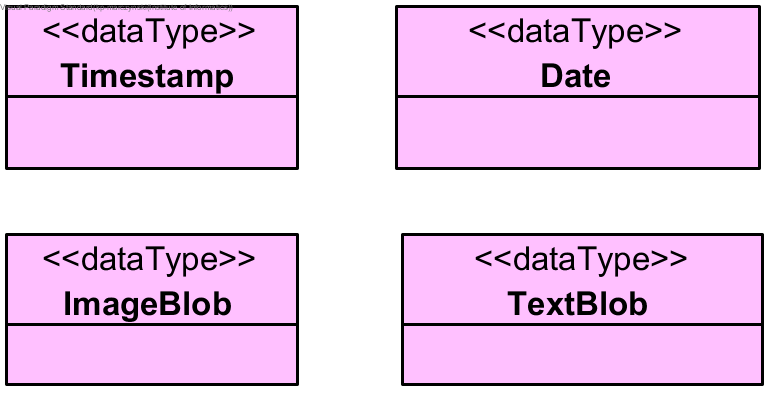
\includegraphics[scale=0.7]{../uml/class_diagrams/dataTypes.png}
        \caption{Typy danych - diagram klas (opr.wł).}\label{rysunek:class-diagram-data-types}
    \end{figure}
\end{minipage}

\begin{minipage}{\textwidth}
    \begin{figure}[H]
        \centering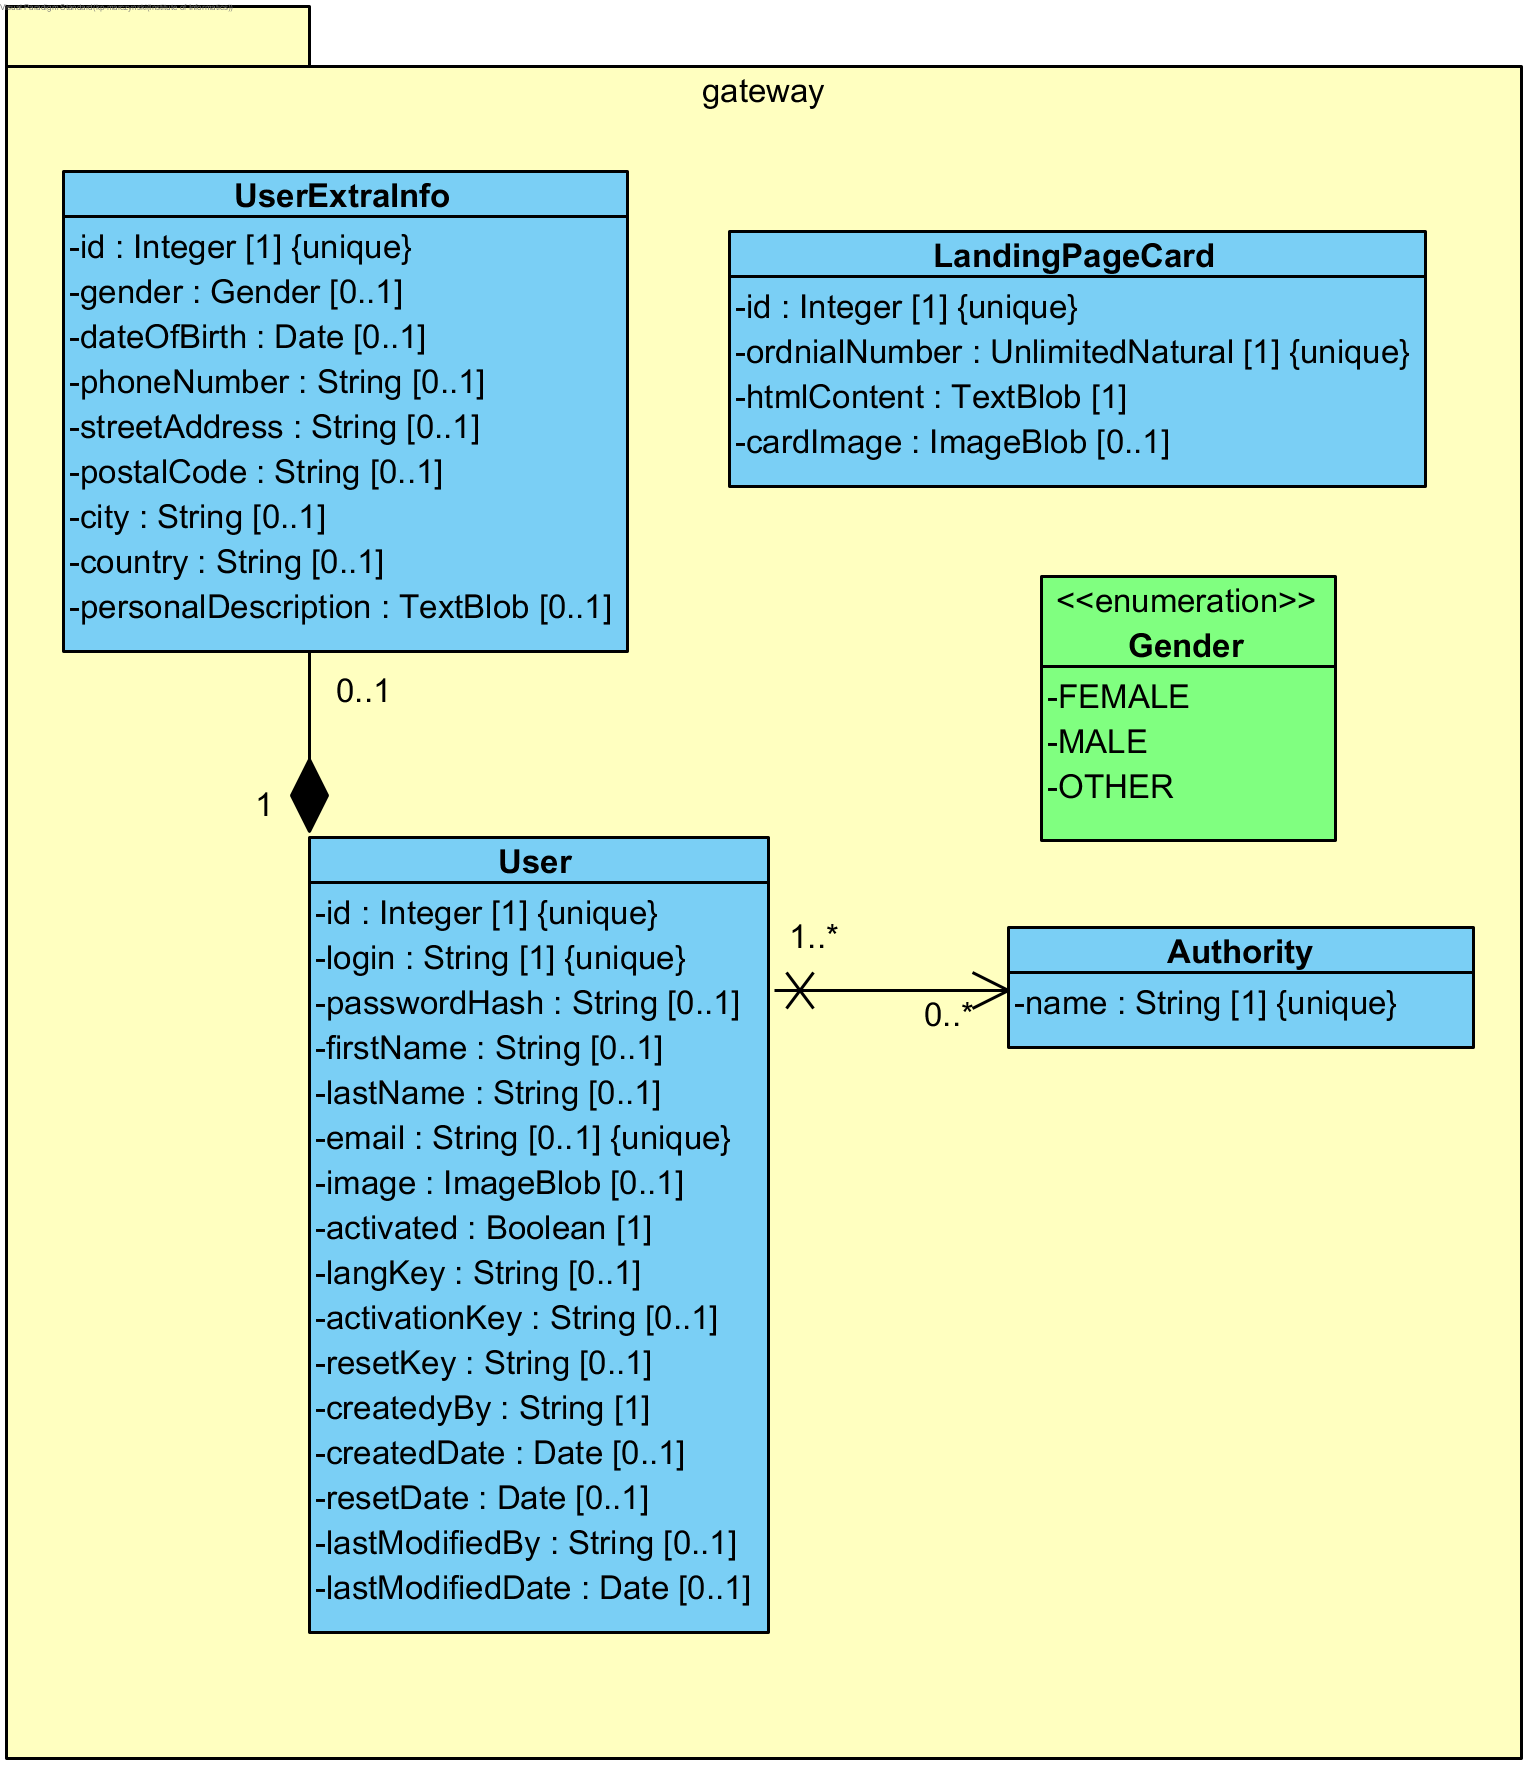
\includegraphics[scale=0.7]{../uml/class_diagrams/gateway.png}
        \caption{Gateway - diagram klas (opr.wł).}\label{rysunek:class-diagram-gateway}
    \end{figure}
\end{minipage}

\begin{minipage}{\textwidth}
    \begin{figure}[H]
        \centering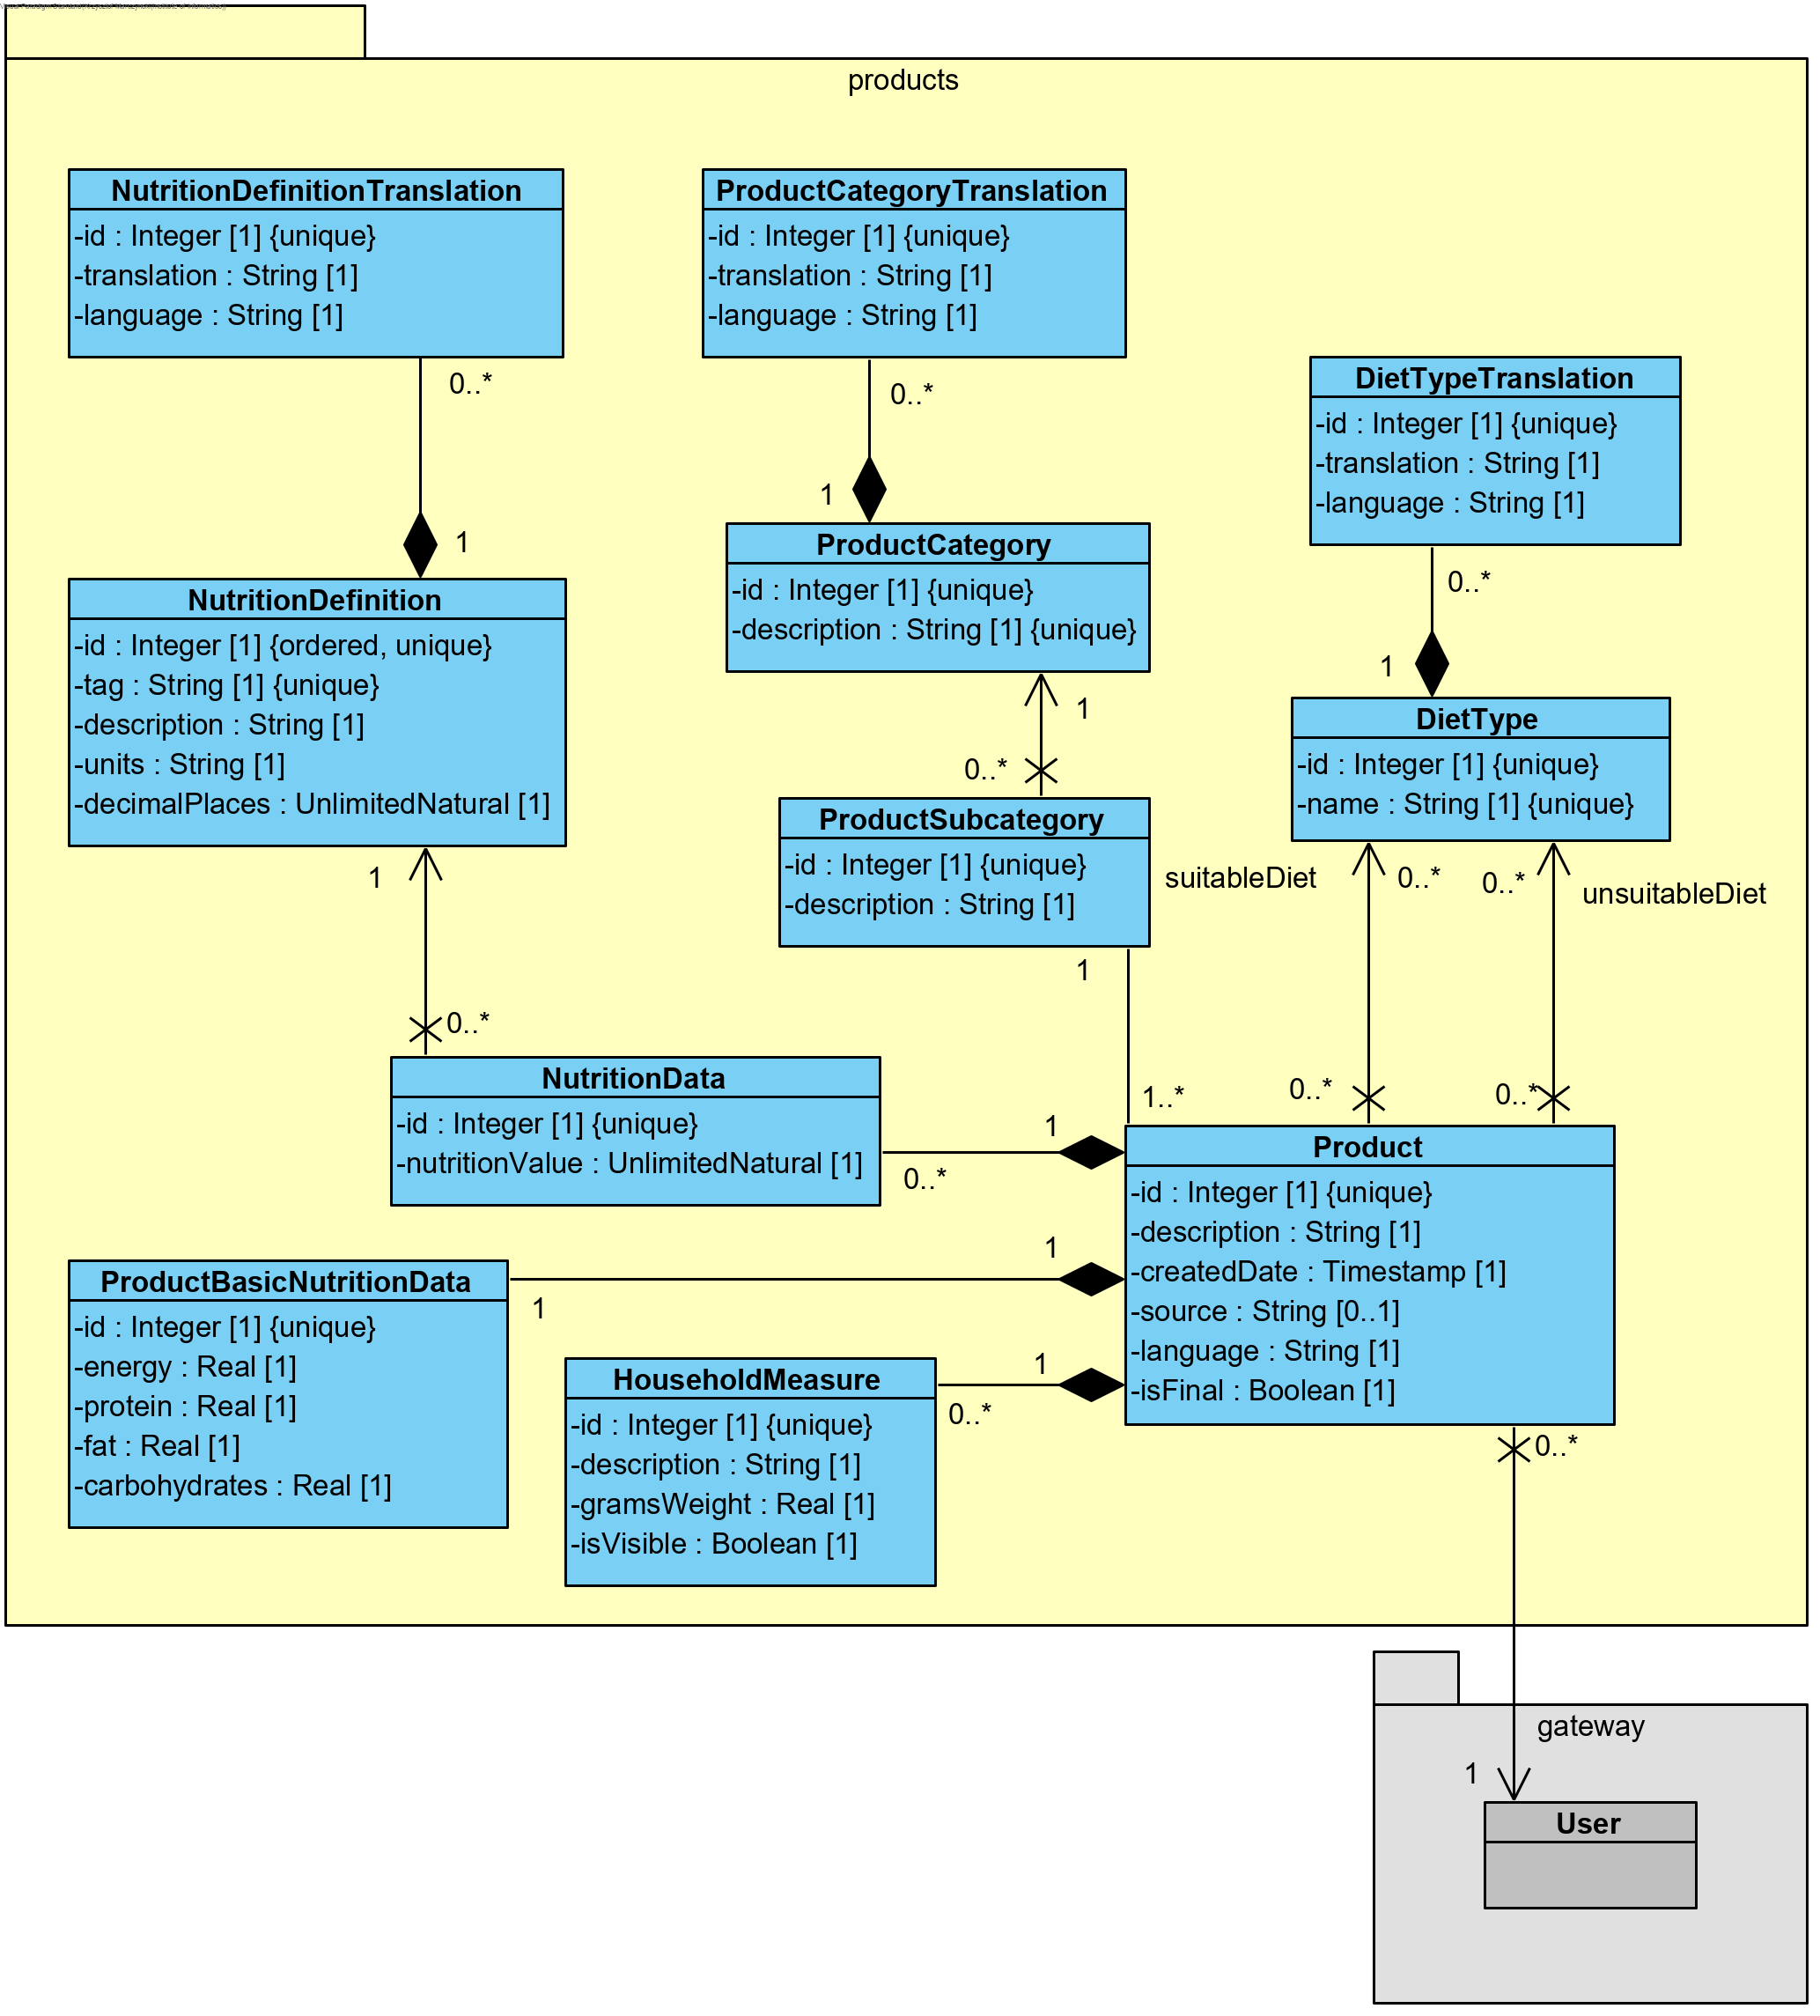
\includegraphics[scale=0.7]{../uml/class_diagrams/products.png}
        \caption{Produkty - diagram klas (opr.wł).}\label{rysunek:class-diagram-products}
    \end{figure}
\end{minipage}

\begin{minipage}{\textwidth}
    \begin{figure}[H]
        \centering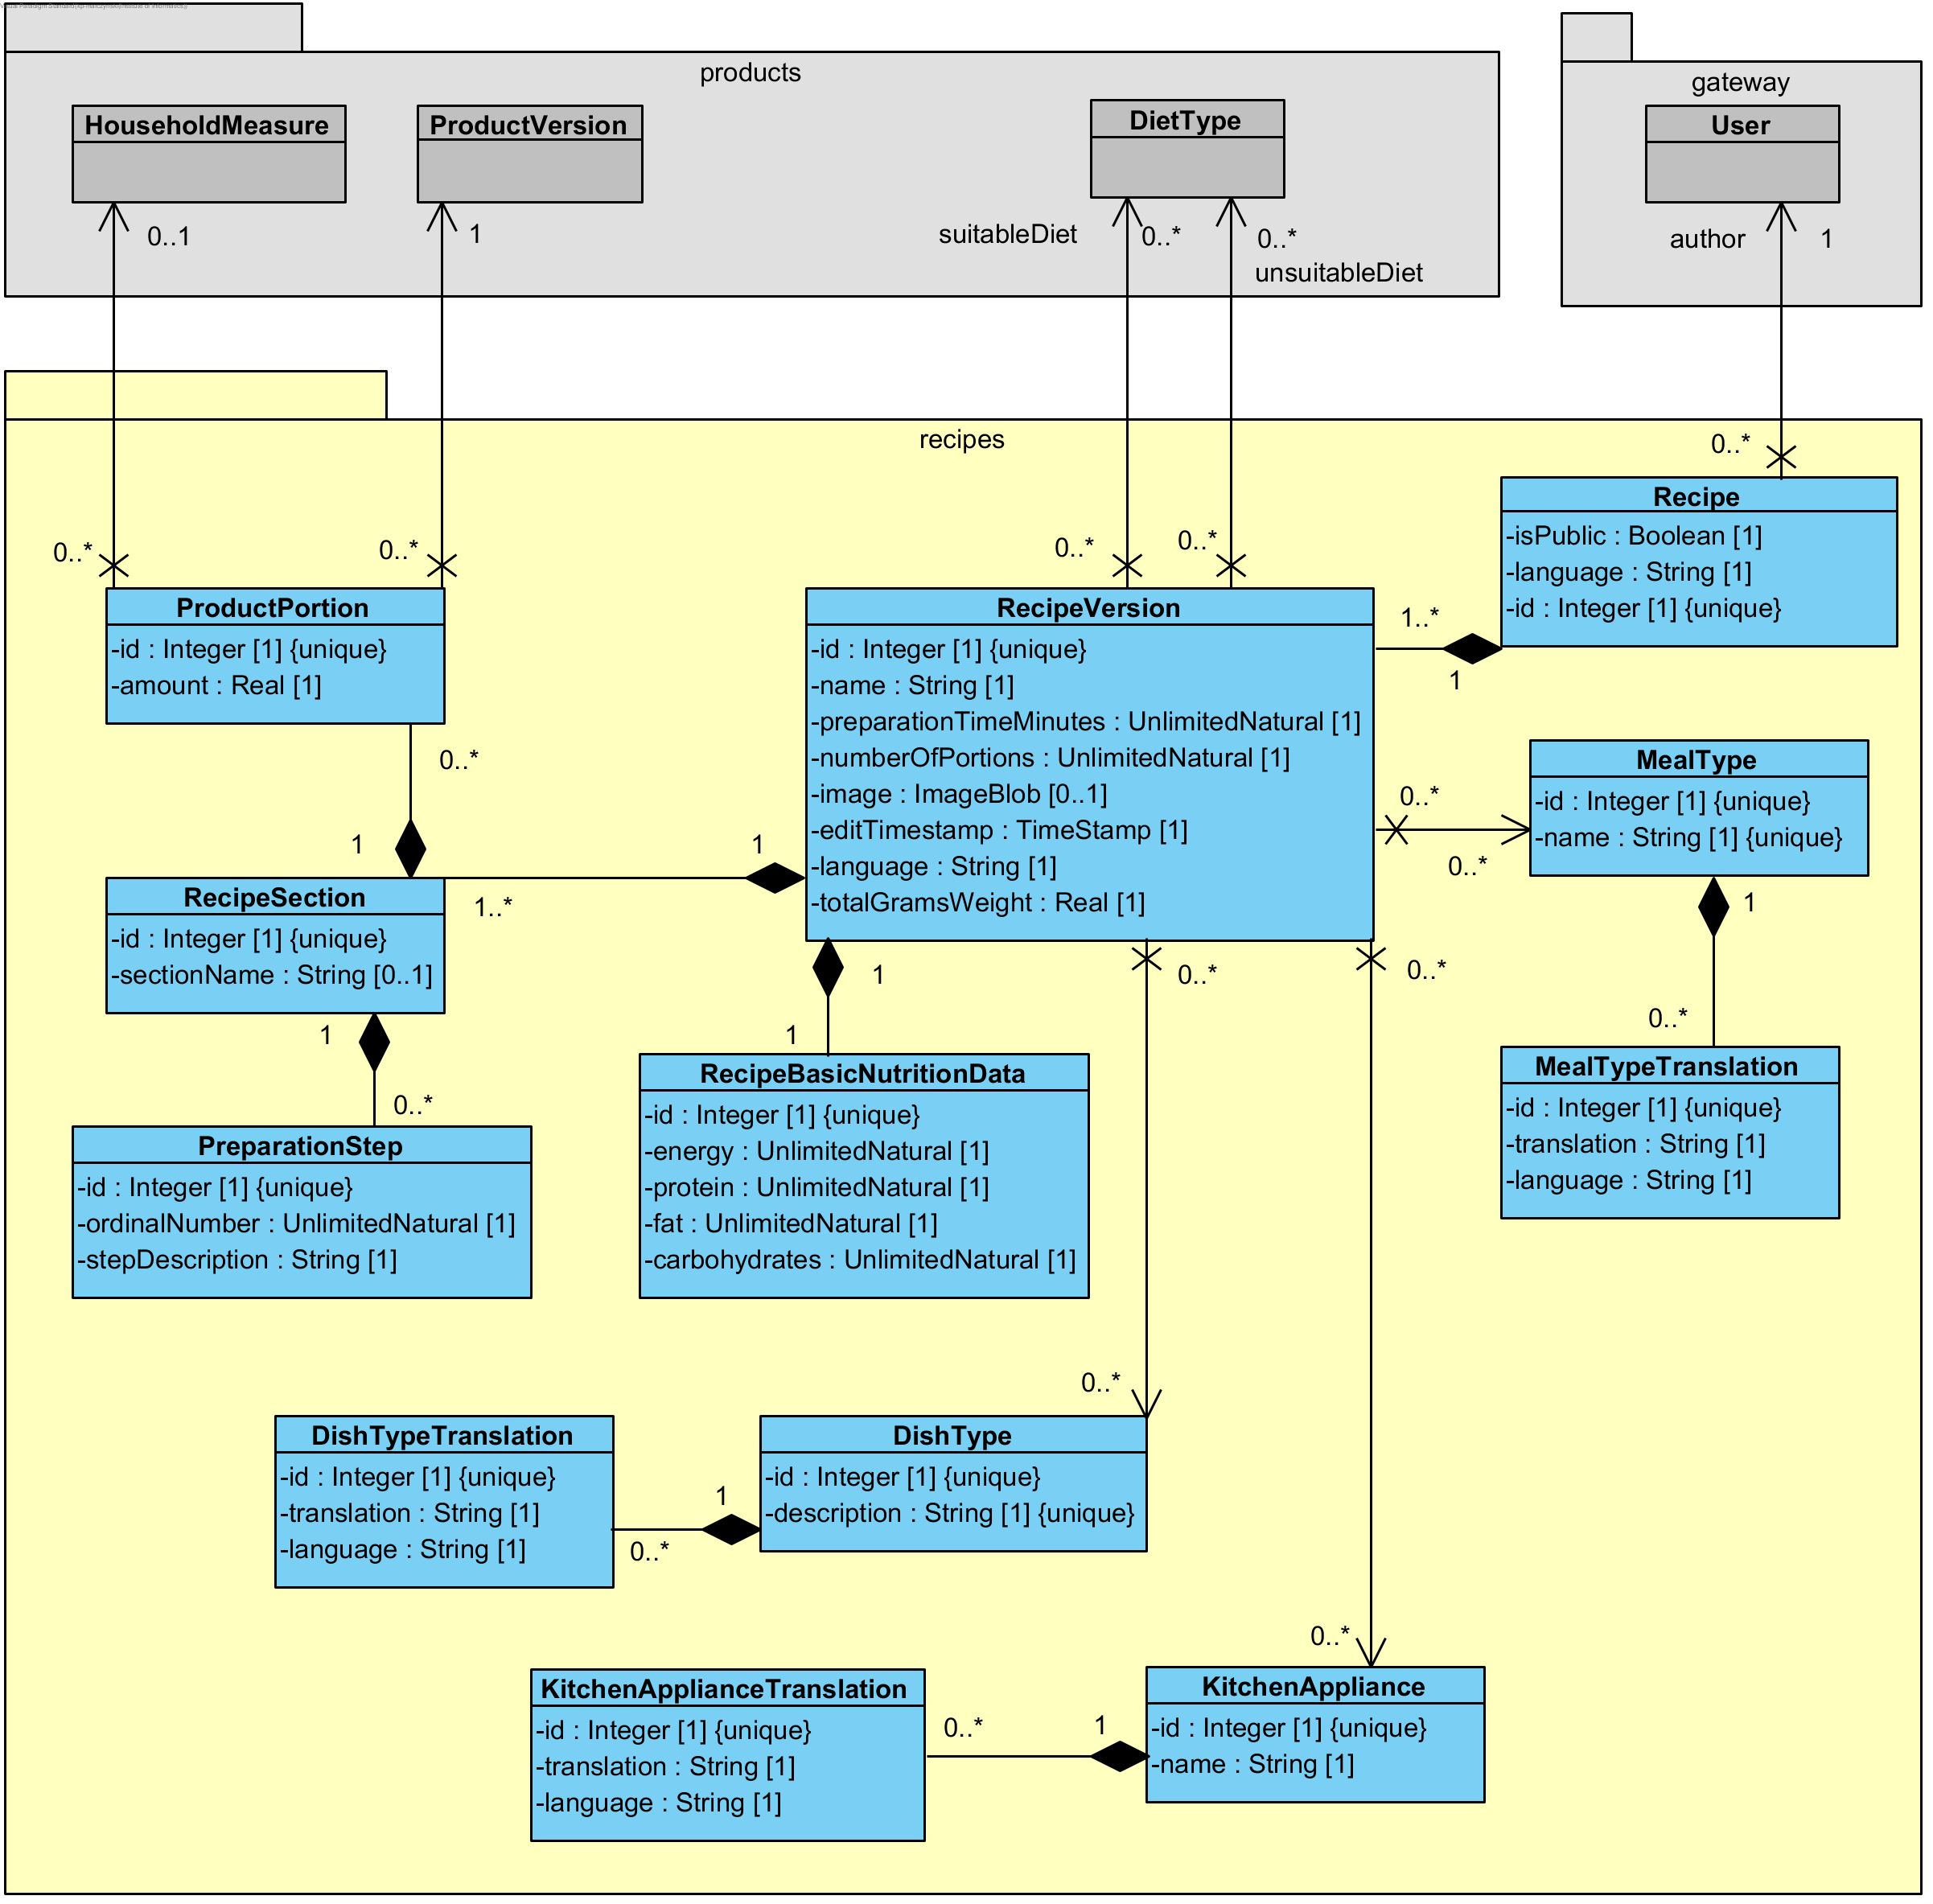
\includegraphics[scale=0.7]{../uml/class_diagrams/recipes.png}
        \caption{Przepisy - diagram klas (opr.wł).}\label{rysunek:class-diagram-recipes}
    \end{figure}
\end{minipage}

\begin{minipage}{\textwidth}
    \begin{figure}[H]
        \centering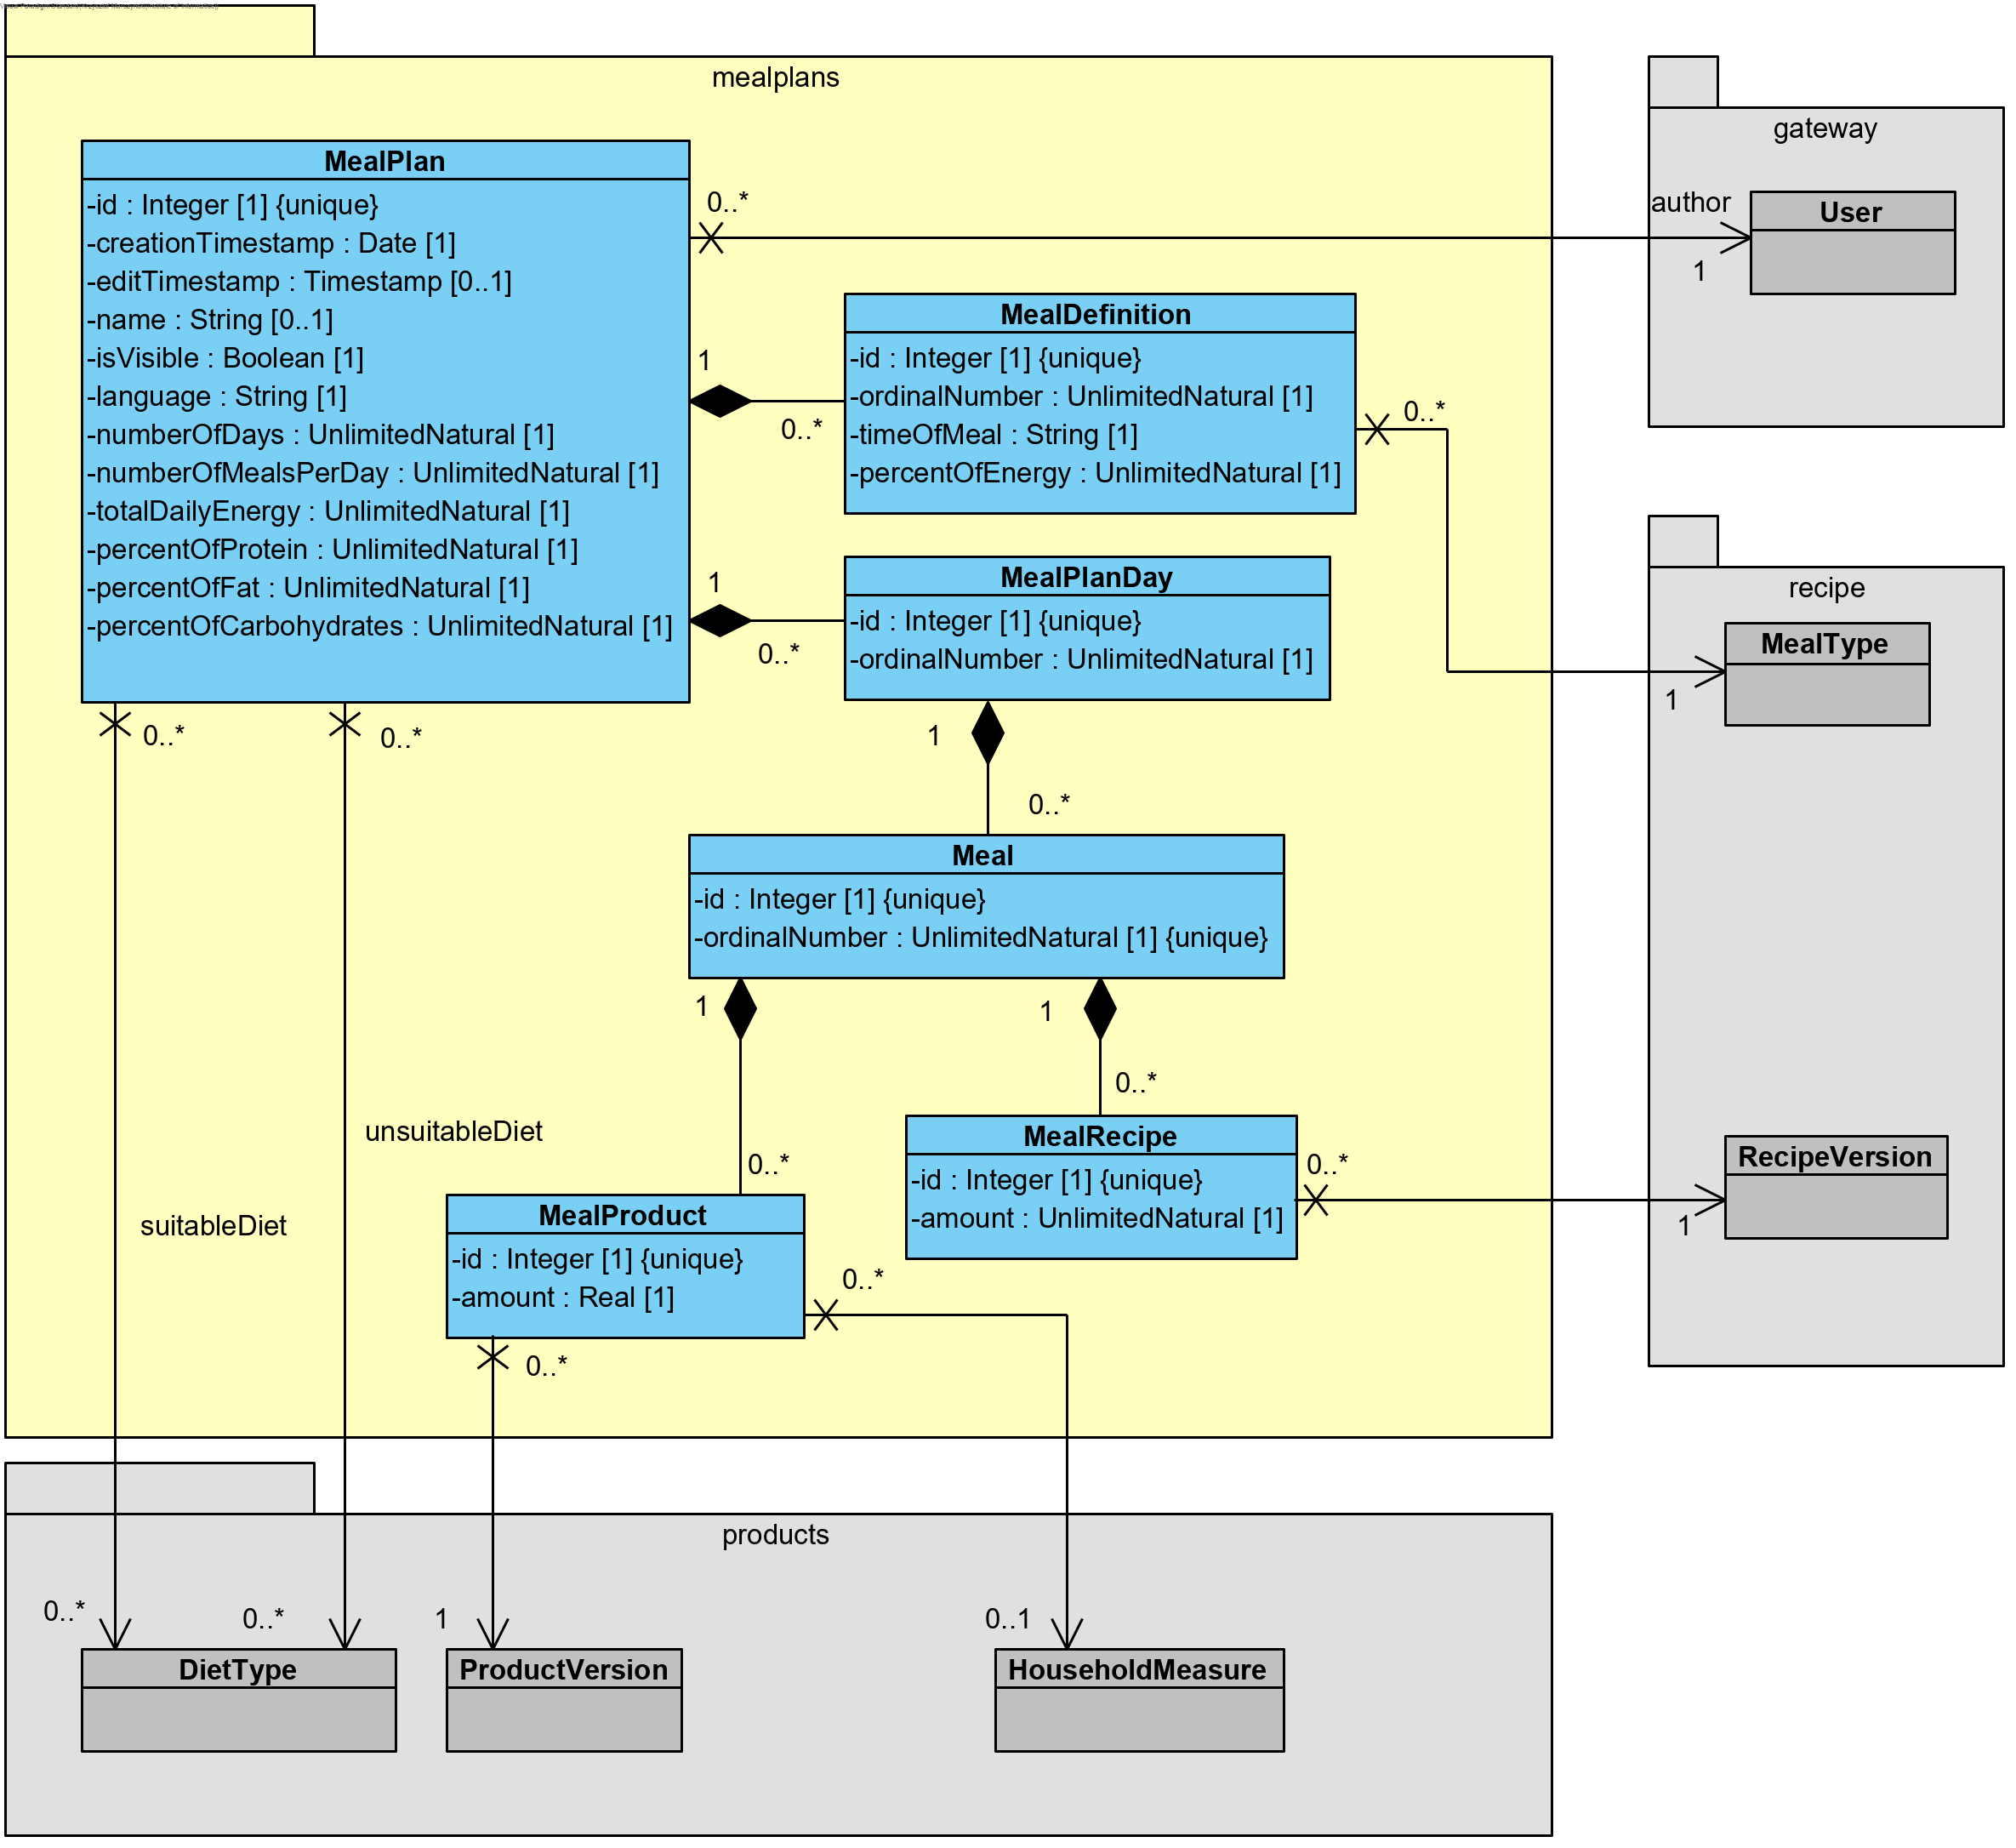
\includegraphics[scale=0.7]{../uml/class_diagrams/mealplans.png}
        \caption{Jadłospisy - diagram klas (opr.wł).}\label{rysunek:class-diagram-mealplans}
    \end{figure}
\end{minipage}

\begin{minipage}{\textwidth}
    \begin{figure}[H]
        \centering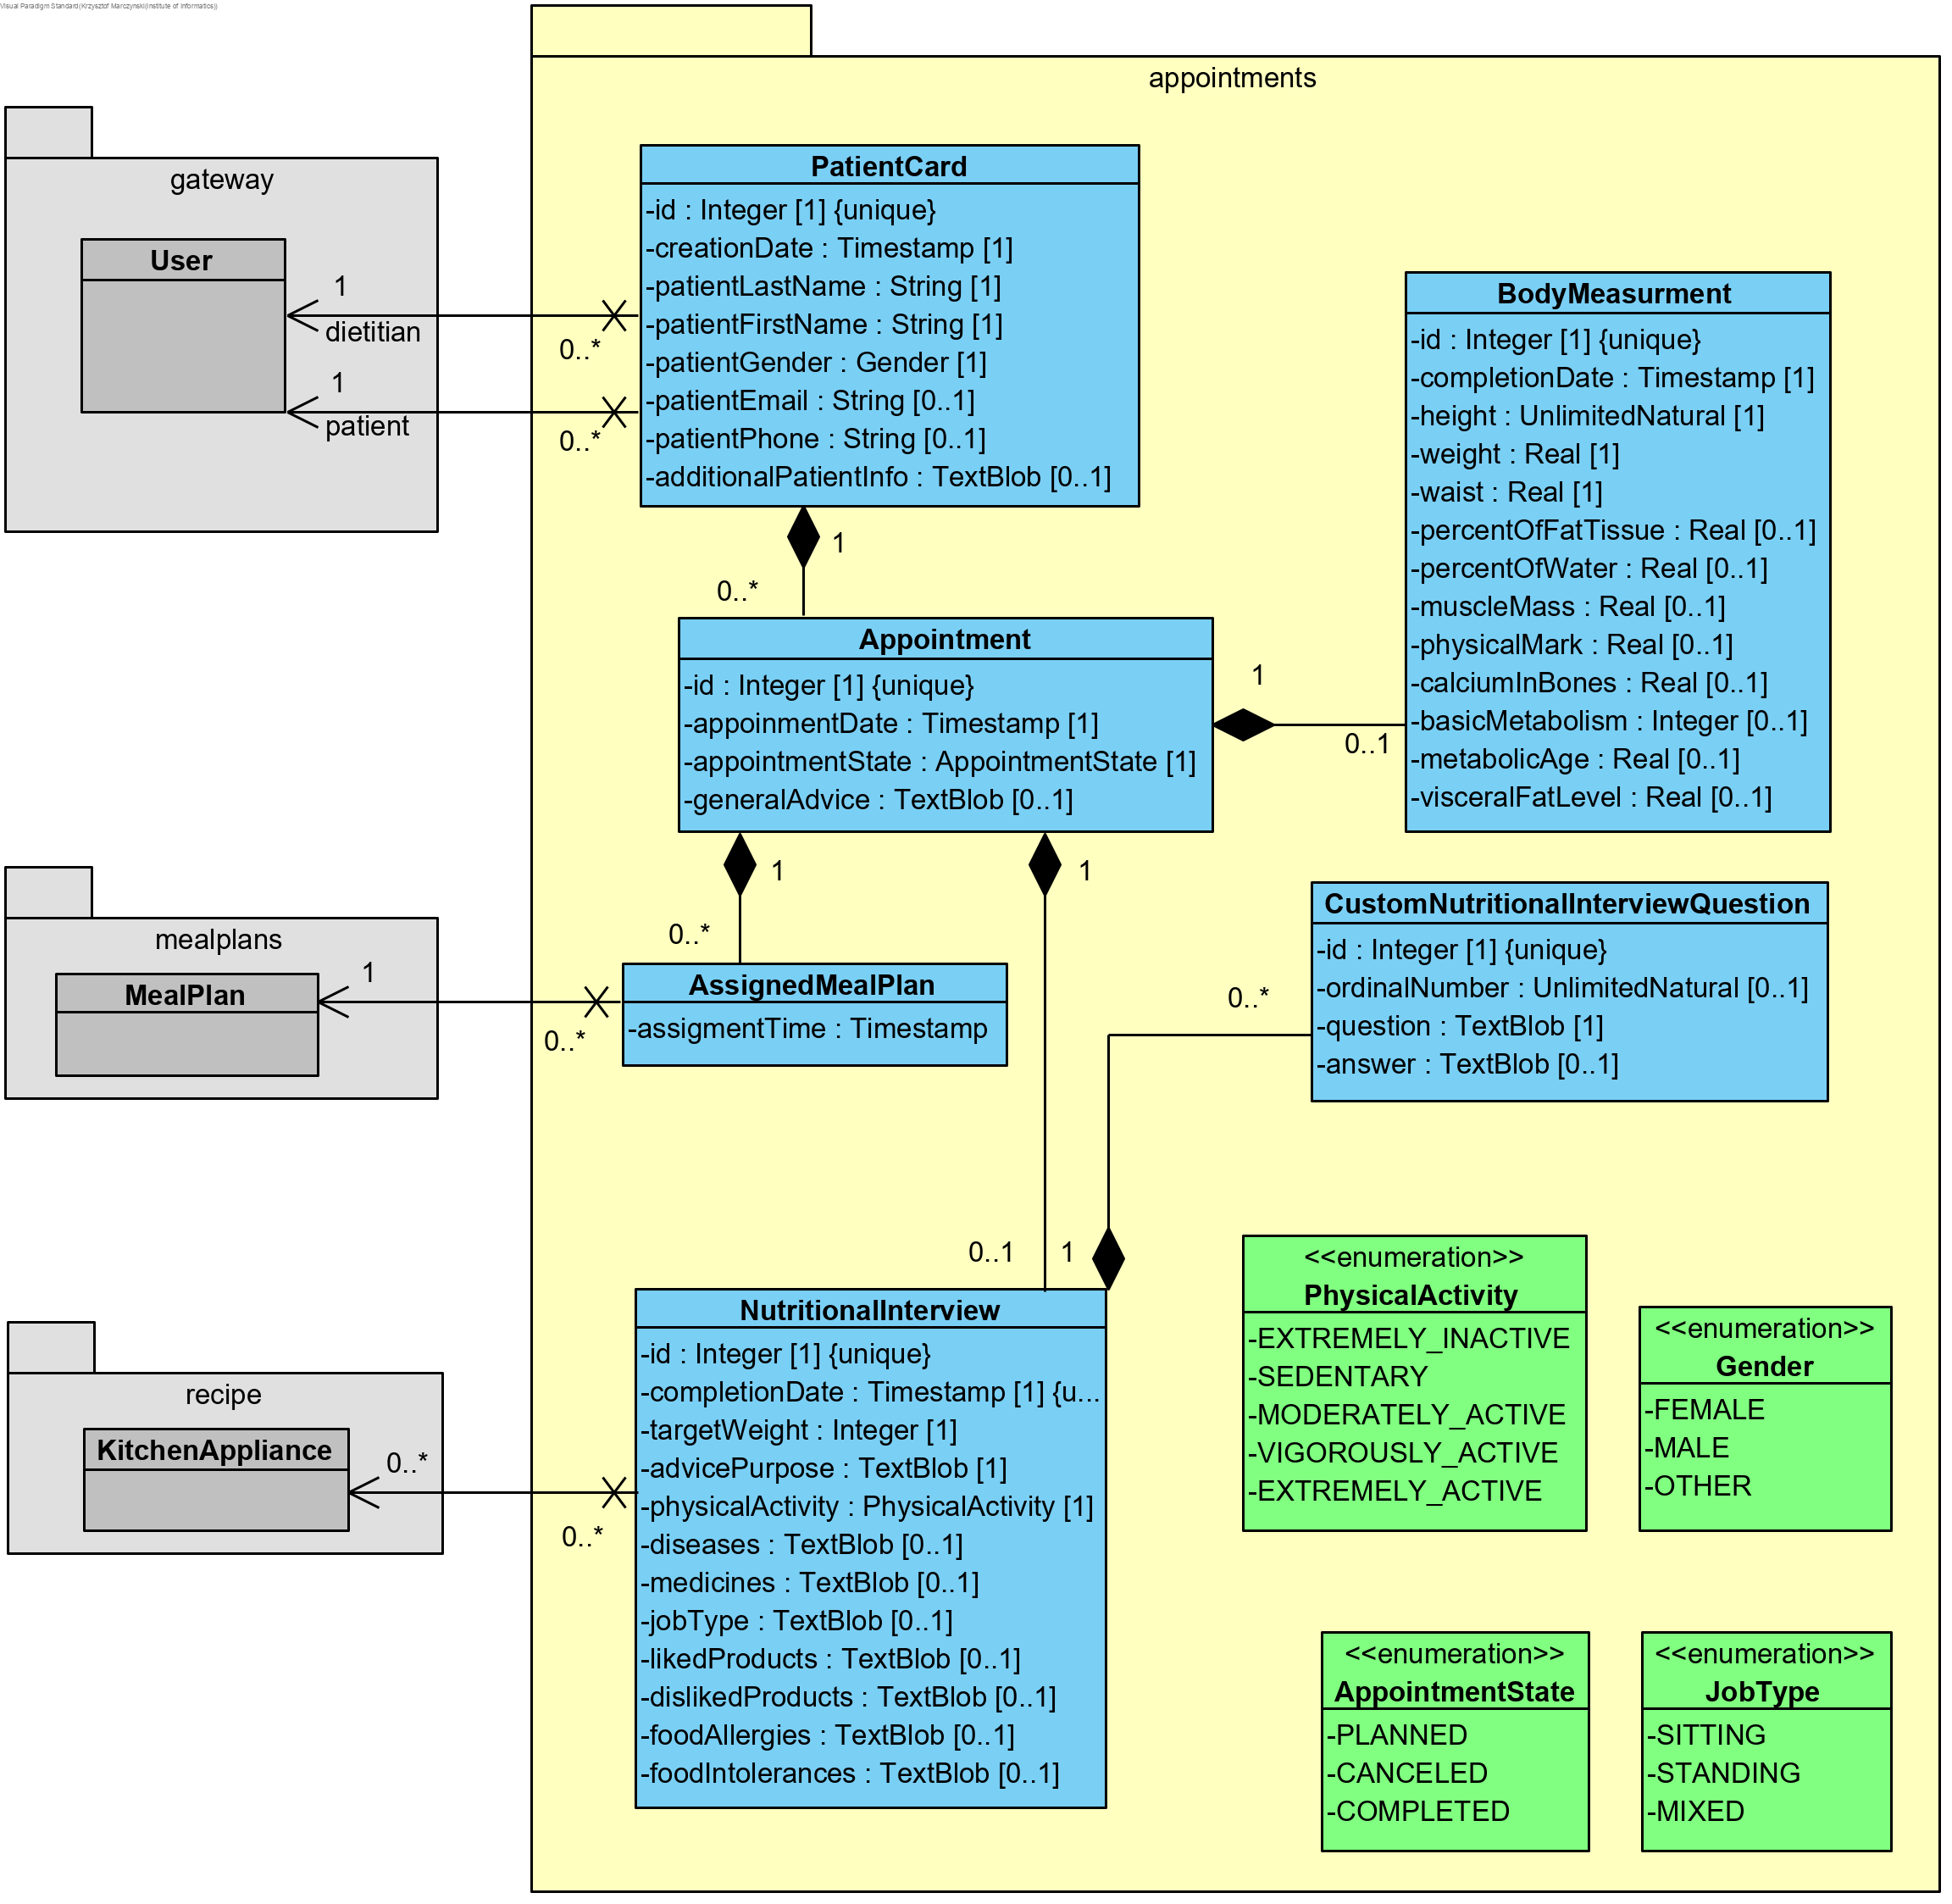
\includegraphics[scale=0.7]{../uml/class_diagrams/appointments.png}
        \caption{Wizyty - diagram klas (opr.wł).}\label{rysunek:class-diagram-appointments}
    \end{figure}
\end{minipage}



\thispagestyle{normal}

\section{Opis podstawowej architektury systemu}
\todo{Opisać, że to aplikacja webowa w architekturze mikroserwisów
Wyszczególnienie modułów;
Diagram rozmieszczenia, wzorce projektowe}

%https://martinfowler.com/eaaDev/TemporalObject.html
\thispagestyle{normal}
